\documentclass[conference,a4paper]{IEEEtran}
\IEEEoverridecommandlockouts
\usepackage[utf8]{inputenc}
\usepackage[T1]{fontenc}
\usepackage{amsmath,amssymb}
\usepackage{graphicx}
\usepackage{textcomp}
\usepackage[table]{xcolor}
\usepackage{booktabs}
\usepackage{tabularx}
\usepackage{array}
\usepackage{placeins}
\usepackage{stfloats}
\usepackage{microtype}
\usepackage{url}
\usepackage{cite}
\usepackage{pdfpages}
\usepackage[hidelinks]{hyperref}
\hypersetup{pdftitle={From Snapshots to Trajectories: Three Visual Analytics Workflows on Global Internet Adoption},
  pdfauthor={Parikshith Aithal K V, Sindhoor Ganapathi Hegde, Varshith M Gowda}}
\graphicspath{{diagrams/}{../images/}}
\extrafloats{100}
\renewcommand{\topfraction}{0.9}
\renewcommand{\dbltopfraction}{0.9}
\renewcommand{\textfraction}{0.07}
\renewcommand{\floatpagefraction}{0.8}
\renewcommand{\dblfloatpagefraction}{0.8}
\setcounter{totalnumber}{4}
\setcounter{dbltopnumber}{2}
\definecolor{loop}{HTML}{C0392B}
\newcolumntype{Y}{>{\raggedright\arraybackslash}X}
\newcommand{\inference}[1]{\par\smallskip\noindent\textit{Inference.} #1\par\smallskip}
\newcommand{\hyp}[2]{\par\smallskip\noindent\textbf{#1}\enspace #2\par\smallskip}

\begin{document}

\title{From Snapshots to Trajectories: Three Visual Analytics Workflows on Global Internet Adoption}

\author{
\IEEEauthorblockN{Parikshith Aithal K V}
\IEEEauthorblockA{Roll No. BT2024249\\IIIT Bangalore}
\and
\IEEEauthorblockN{Sindhoor Ganapathi Hegde}
\IEEEauthorblockA{Roll No. BT2024014\\IIIT Bangalore}
\and
\IEEEauthorblockN{Varshith M Gowda}
\IEEEauthorblockA{Roll No. BT2024227\\IIIT Bangalore}
}
\maketitle

\begin{abstract}
Assignment~1 (A1, appended) concluded visually that mobile phones let many countries skip the
fixed-line era, but that broadband rather than mobile saturation separates connected from
unconnected populations. This report tests that conclusion with three visual analytics (VA)
workflows in the sense of Keim et~al.~\cite{keim2008scope}, one per family of methods and one per team
member, each drawn unrolled with its question, hypotheses, plugged-in visualizations, analysis path
and a single labelled feedback loop. In the statistical workflow (W1), logistic diffusion fits and
rank tests show take-off delays of 6--12 years, and the feedback loop re-expresses every curve in its
own time and scale: aligned at their take-off years, 201 country curves collapse onto one S-curve and
the cross-country spread falls from 32 to 10 percentage points; a direct test then shows that countries
which skipped landlines are saturated on mobile yet only 44\% online (93\% where landlines were built). In
the unsupervised workflow (W2),
bootstrap co-assignment and anomaly persistence show that 2024 snapshot clusters are only moderately
stable (ARI 0.64) and that Fiji's anomaly is a transient recording artefact; the feedback loop turns
snapshots into 26-year trajectories compared by dynamic time warping, which regroups 37 of 133
countries into three path archetypes. In the supervised workflow (W3), history features defined by
W1's inferences and in-fold imputation lower country-grouped error on identical rows from 11.77 to
10.16 points; a drift chart then shows a post-2020 shift that explains why raw 80\% forecast
intervals cover only 50\%, and conformal re-calibration restores 83\%. Combined, the workflows answer
A1's question: the digital divide is a delay on a common S-curve that is narrowing only in relative
terms, and fixed infrastructure, not mobile, marks a country's position on it.
\end{abstract}

\begin{IEEEkeywords}
visual analytics, feedback loop, diffusion curves, convergence, clustering, dynamic time warping,
conformal prediction, data drift, digital divide
\end{IEEEkeywords}

% =========================================================================================
\section{Introduction}
% =========================================================================================
\subsection{From A1 to A3}
A1 asked whether mobile technology let countries skip fixed-line infrastructure, whether that
closed the connectivity gap, and, if not, what separates connected populations from unconnected
ones. Its answer was visual: a landline count today hides opposite histories (A1 Fig.~5), the gap
between income groups widened (A1 Fig.~11), subscriptions are not people (A1 Figs.~10 and~18), and
broadband correlates more strongly with adoption than mobile does (A1 Figs.~19--20). Visual
readings of this kind can be confounded by time trends, outliers and recording errors. A3 therefore
tests them with statistics and models placed inside VA workflows, in which visualization and
automated analysis alternate and each informs the next~\cite{keim2008challenges,card1999,sacha2014}.

\subsection{Main question and the three workflows}
The main A3 question is: \emph{can infrastructure and history explain and forecast which countries
get online, and does feeding each iteration's inferences back into the data change the answer?} It
is answered by three workflows (Fig.~\ref{fig:v0}). Each is a complete, unrolled Keim loop with its
own question, hypotheses, two iterations and one feedback loop, and each uses one family of methods
required by the brief:
\begin{itemize}
\item \textbf{W1, statistical analysis} (Fig.~\ref{fig:w1}). Q1: when did each country take off, is
  the gap closing, and do the indicators measure what they appear to measure?
\item \textbf{W2, unsupervised mining} (Fig.~\ref{fig:w2}). Q2: which kinds of countries exist, how
  stable are those kinds, and which countries fit none of them?
\item \textbf{W3, supervised learning} (Fig.~\ref{fig:w3}). Q3: how well does infrastructure predict
  internet use in unseen countries and unseen years, and how far can the forecast be trusted?
\end{itemize}
The workflows are not independent: W1's and W2's inferences define the shared artefact rule, and W1's
inferences define the features that W3 learns from. A synthesis combines their knowledge into one
answer (Section~\ref{sec:k2}).

\subsection{Contributions}
The report contributes (i) three unrolled Keim workflows, each with its question and hypotheses
written on the diagram, its visualizations plugged into the stages that produced them, its analysis
path numbered, and one labelled feedback loop that transforms the data rather than filtering it;
(ii) a statistical re-test of A1's visual claims, including a re-expression of every adoption curve in
its own time that turns ``years behind'' into a tested delay; (iii) stability and persistence evidence
that separates structural anomalies from recording artefacts; (iv) a leakage-safe comparison of the
supervised iterations on identical rows and folds; (v) a drift chart that links forecast
mis-calibration to a post-2020 shift, with a calibration curve for the re-calibrated intervals; and
(vi) a reproducible pipeline (Section~\ref{sec:repro}) with an interactive demonstrator that runs in a web
browser.

\begin{figure*}[!t]
\centering
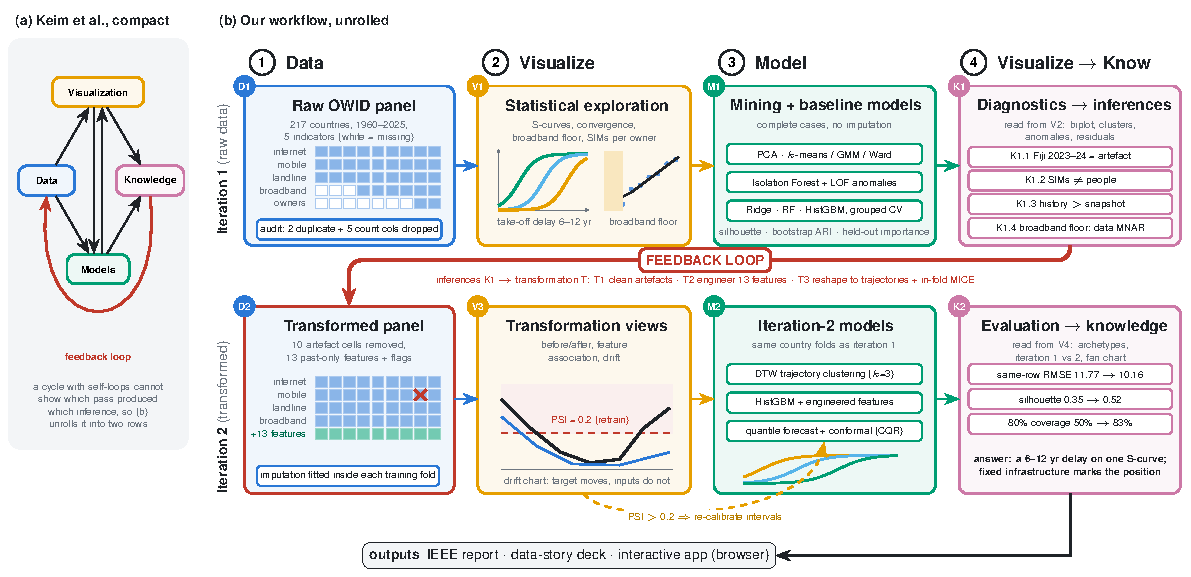
\includegraphics[width=\textwidth]{V0_workflow_architecture.pdf}
\caption{\textbf{V0: one main question, three unrolled workflows, one synthesis.} Each lane is a
complete Keim loop: iteration~1 on raw data (visualization and model, with the key figure plugged in),
inferences $K_1$, the feedback-loop transformation $T$ (red), iteration~2 on the transformed data and
knowledge $K_2$. The compact Keim diamond (top right) is shown for reference; unrolling removes its
self-loops, so each red edge is the single feedback loop of one workflow. Bold notes mark knowledge
passed between workflows; all three feed the synthesis $K^\ast$ (V14). The full workflows are
Figs.~\ref{fig:w1}--\ref{fig:w3}.}
\label{fig:v0}
\end{figure*}

\subsection{Organisation}
Section~\ref{sec:related} reviews related work and Section~\ref{sec:data} the data and its quality.
Section~\ref{sec:methods} describes the workflow design and every method, and Section~\ref{sec:design}
justifies the visual encodings. Sections~\ref{sec:w1}, \ref{sec:w2} and~\ref{sec:w3} report the three
workflows, and Section~\ref{sec:disc} combines them, answers the main question and discusses validity.

% =========================================================================================
\section{Related Work}\label{sec:related}
% =========================================================================================
\textit{VA process models.} Card et~al.~\cite{card1999} describe visualization as a pipeline from
data to view; Keim et~al.~\cite{keim2008scope,keim2008challenges} extend it to the VA diamond, in
which data, visualization, models and knowledge are linked by transitions and a feedback loop.
Sacha et~al.~\cite{sacha2014} refine the knowledge side into exploration, verification and
knowledge-generation loops, and stress that hypotheses and the analyst's path are part of the
process; the numbered paths and hypothesis tables of Figs.~\ref{fig:w1}--\ref{fig:w3} record exactly
these. Wang et~al.~\cite{wang2024va4ml} survey VA for machine learning from a data perspective, and
the data-centric tasks they identify (diagnosing data, improving data, explaining models) are the
tasks of the feedback loops here. Javed and Elmqvist~\cite{javed2012composite} classify composite
views into juxtaposed, superimposed, overloaded, nested and integrated designs, which
Section~\ref{sec:design} uses.

\textit{Diffusion and the digital divide.} Technology adoption is classically modelled as an
S-shaped diffusion curve~\cite{rogers2003}. Comin and Hobijn~\cite{comin2010} show that cross-country
differences in adoption are dominated by adoption \emph{lags} rather than by different curve shapes,
which W1 tests for the internet. The ITU~\cite{itu2023} reports that a third of the world remained
offline in 2023, concentrated in low-income countries, consistent with the late-starter archetype
found in W2.

\textit{Clustering stability, time-series mining and uncertainty.} Consensus
clustering~\cite{monti2003consensus} measures how often two items are grouped together over resampled
data, and the cophenetic correlation~\cite{sokal1962cophenetic} measures how faithfully a dendrogram
preserves distances. Dynamic time warping~\cite{sakoe1978dtw} is a standard distance for clustering
curves that are similar in shape but shifted in time~\cite{aghabozorgi2015}. Concept drift, a change in
the relation between inputs and target over time, invalidates models trained on earlier
data~\cite{gama2014}. Conformalised quantile regression~\cite{romano2019cqr} gives prediction intervals
with finite-sample coverage under exchangeability, and the Population Stability Index~\cite{siddiqi2006}
is a common drift monitor in deployed ML workflows.

% =========================================================================================
\section{Data and Pre-processing}\label{sec:data}
% =========================================================================================
\subsection{Core dataset}
The core data are A1's merged OWID panel~\cite{owid}: 247 entities over 1960--2025. Removing
aggregate rows (World, income groups, continents) leaves 217 countries and 12{,}579 country-years.
Table~\ref{tab:vars} lists the five indicators. Internet users is the target of every supervised
model. Regions follow A1's six-continent lookup, so A1 and A3 groupings coincide.

\begin{table}[!t]
\centering
\caption{Indicators analysed (country rows only)}
\label{tab:vars}
\footnotesize
\begin{tabularx}{\columnwidth}{@{}Y l r r r@{}}
\toprule
Indicator & Years & Rows & Obs.\,\% & Median \\
\midrule
Internet users (\% pop.), target & 1990--2025 & 6{,}224 & 49.5 & 19.0 \\
Mobile subscriptions /100 & 1960--2024 & 10{,}594 & 84.2 & 1.7 \\
Phone owners (\% adults) & 2013--2025 & 1{,}330 & 10.6 & 85.3 \\
Fixed telephone lines /100 & 1960--2024 & 11{,}794 & 93.8 & 6.6 \\
Fixed broadband /100 & 1998--2024 & 4{,}330 & 34.4 & 4.7 \\
\bottomrule
\multicolumn{5}{@{}l}{\scriptsize Obs.\,\%: share of the 12{,}579 country-years observed. Source:~\cite{owid}.}
\end{tabularx}
\end{table}

\subsection{Pre-processing beyond A1}
\textit{Audit.} Two columns are exact copies of others: \texttt{internet\_users\_share\_pct\_ict}
duplicates the target and \texttt{broadband\_penetration\_per100} duplicates broadband
subscriptions (maximum absolute difference 0). The pipeline asserts this before dropping them. Five
count columns are dropped because they scale with population, and the internet-user count is the
target multiplied by population.

\textit{No imputation in iteration~1.} Every first iteration uses complete cases only, so every
pattern it reports exists in observed data. Imputation enters only in W3's second iteration, after
the quality analysis below motivates it, and is always fitted on the training fold alone.

\textit{Supplementary data.} None is used. A World Bank income join was considered and rejected for
the same reason as in A1: the question concerns infrastructure, and adding income would answer a
different question. The consequence, that all results are associations, is discussed in
Section~\ref{sec:limits}.

\subsection{Data quality and missingness (W1, before step 1)}
Coverage was measured against all 217 countries. Mobile subscriptions and landlines
are observed for more than 95\% of countries from 1990 to 2022; broadband begins around 2000 and
passes 80\% only in 2005; ownership exists only in survey years from 2014; and 2023--2025 thin out
sharply, which is why the snapshot year is 2024 and the forecast horizon ends in 2025. Coverage is
lowest in Oceania for every indicator. Missingness is not random: in 2015--2024 the median internet
share is 50\% in country-years without an ownership survey and 75\% in those with one
(Mann--Whitney $p=10^{-41}$); for broadband the gap is smaller (63\% against 70\%, $p=10^{-4}$).

\inference{Imputing ownership with a global mean would bias low-connectivity countries upwards.
The first iterations therefore use complete cases only, and W3's second iteration uses multivariate
imputation fitted in-fold together with explicit missingness flags, so the model can learn that a
missing survey is itself informative.}

% =========================================================================================
\section{Workflow Design and Methods}\label{sec:methods}
% =========================================================================================
\subsection{Unrolled workflows and the evidence they carry}
Keim et~al.~\cite{keim2008scope,keim2008challenges} describe VA as transitions between four stages,
data ($D$), visualization ($V$), models ($M$) and knowledge ($K$), with a feedback loop from
knowledge back to data. Drawn as a state diagram (Fig.~\ref{fig:v0}, top right) the process is a
cyclic graph with self-loops, which cannot show which pass produced which inference. Each workflow is
therefore unrolled into two iterations, $D_1\!\rightarrow\!V_1\!\rightarrow\!M_1\!\rightarrow\!K_1$ on
raw data and $D_2\!\rightarrow\!V_2\!\rightarrow\!M_2\!\rightarrow\!K_2$ on transformed data, joined by
a single edge labelled \textcolor{loop}{\textbf{Feedback loop}} that carries the transformation $T$.
Table~\ref{tab:criteria} lists the four properties that the workflow diagrams are designed to show and
where each is shown.

\begin{table}[!t]
\centering
\caption{What each workflow diagram is designed to show, and where}
\label{tab:criteria}
\footnotesize
\begin{tabularx}{\columnwidth}{@{}p{2.25cm} Y@{}}
\toprule
Property & How it is shown \\
\midrule
Evidence of the workflow & the figures that produced each inference are plugged into the $V$ stage
of the iteration that produced them (thumbnails in Figs.~\ref{fig:w1}--\ref{fig:w3}) \\
A feedback loop that transforms the data & every $T$ changes the representation (own time and scale;
snapshot to trajectory under a new distance; new predictors and rows), not only a filter
(Table~\ref{tab:loops}) \\
Questions and hypotheses & written at the top of each diagram with the test and verdict, and repeated
at the start of each workflow section \\
The analysis path & figures are numbered in the order they were read; the path line under each
diagram and the ``Analysis path'' paragraphs record why each step followed the last \\
\bottomrule
\end{tabularx}
\end{table}

\begin{table*}[!t]
\centering
\caption{The three feedback loops: inference, evidence, the transformation it triggers, and why the
transformation is more than a filter}
\label{tab:loops}
\footnotesize
\begin{tabularx}{\textwidth}{@{}l p{3.4cm} Y Y p{3.0cm}@{}}
\toprule
& Inference ($K_1$) & Evidence & Transformation $T$ (input to iteration~2) & Why it is significant \\
\midrule
W1 & K1.1 Fiji's 2023--24 mobile values are an artefact & 111$\rightarrow$574 per 100 with flat
ownership (V3); transient anomaly in W2 (V6b) & \textbf{T1} two rules for every country: (A) a
saturated market ($\ge$90) exceeding 2.5 times its five-year median; (B) a one-year jump of $\ge$1.8
times that reverts within 1.25 times. Ten cells removed & a rule, not a hand edit; applies to all
countries and indicators \\
& K1.2 Subscriptions overstate people & $\rho$ 0.52 against 0.89 (V3); importance near zero (V7) &
\textbf{T2} SIMs per owner, multi-SIM flag (1.5), mobile capped at 100 & new measurement scale \\
& K1.3 Calendar-time levels mix \emph{when} with \emph{how far} & take-off delays (V1); Gini 0.81$\rightarrow$0.19 while the s.d.\
rose until 2013 (V1e) & \textbf{T3} each curve re-indexed to years since its take-off, $t-t_0$, and divided
by its saturation $L$; \textbf{T4} headroom $h=(y_{2024}-y_{2014})/(100-y_{2014})$ & new coordinate
system for every series \\
& K1.4 Broadband has a floor; data are missing not at random & floor holds 29\% of rows (V2); MNAR test
(Mann--Whitney $p=10^{-41}$) & \textbf{T5} $\log(1+\text{broadband})$, floor flag; missingness flags (used by W3) & non-linear
re-expression \\
\midrule
W2 & K1.1 Snapshot clusters are only moderately stable & ARI 0.64, mixed and legacy co-assigned in 46\%
of resamples (V5b); 15 border countries (silhouette $<0.10$) & \textbf{T2} snapshot $\rightarrow$ trajectory: each
country becomes its 2000--2025 internet curve (181 countries, interior gaps interpolated) & a new data
representation \\
& K1.2 Fiji is a transient anomaly; Monaco and Hong Kong are structural & flagged 2 of 6 years versus 6
of 6 (V6b); one indicator each (V6c) & \textbf{T1} shared artefact rule (above); structural anomalies
kept & separates error from real behaviour \\
& K1.3 One year cannot show a path & same level, different histories (A1 Fig.~5) & \textbf{T3}
Euclidean $\rightarrow$ dynamic time warping, Sakoe--Chiba band 5 years; average linkage & a new
distance, invariant to time shifts \\
\midrule
W3 & K1.1 Broadband alone carries the model & permutation importance (V7) & \textbf{T2} 13 past-only
features defined by W1's $K_1$: landline peak and decline, leapfrog index, years since mobile overtook
landlines, per-owner and capped mobile, log broadband, floor flag, momentum & new predictors encoding
history \\
& K1.2 Errors are largest where histories differ & residuals by level (V7) & (as above) & \\
& K1.3 Complete cases drop rows missing not at random & MNAR test in W1 ($p=10^{-41}$) & \textbf{T3} MICE fitted inside each
training fold, with missingness flags: 2{,}134 more rows & new rows, no leakage \\
& (inner loop) the target drifts after 2020 & PSI 0.44 (V13) & \textbf{T4} conformal re-calibration
of the forecast intervals & intervals re-derived \\
\bottomrule
\end{tabularx}
\end{table*}

All engineered features are predictor-only and past-only: none uses the target, and none at year $t$
uses a value after $t$. W2's trajectory clusters are built from the target's own curve and are
therefore not used as a supervised feature.

\subsection{Statistical methods (W1)}
\textit{Diffusion.} Each country's internet share $y(t)$ is fitted, from 1990 onwards and for
countries with at least 15 observed years, by non-linear least squares to
\begin{equation}
y(t)=\frac{L}{1+e^{-k\,(t-t_0)}},
\end{equation}
where $L$ is the saturation level, $k$ the growth rate and $t_0$ the take-off year at which half of
$L$ is reached~\cite{rogers2003}. Regional differences in $t_0$ are tested with Kruskal--Wallis and
pairwise Mann--Whitney tests against Europe, with Holm's correction~\cite{kruskal1952,holm1979}.

\textit{Alignment (iteration~2).} Each series is re-expressed as $\tilde y(a)=100\,y(t_0+a)/L$, the
share of its own saturation $a$ years after its own take-off. If the divide is a pure delay, the
curves $\tilde y(a)$ of all countries coincide; the test statistic is the mean cross-country
interquartile range (IQR) over $a\in[-10,10]$, compared with the same statistic in calendar years.

\textit{Convergence.} $\sigma$-convergence is the decline over time of the cross-country standard
deviation and of the Gini coefficient $G=\sum_i\sum_j|y_i-y_j|/(2n^2\bar y)$. $\beta$-convergence is
assessed on headroom: the share of the remaining gap closed between 2014 and 2024,
$h=(y_{2024}-y_{2014})/(100-y_{2014})$, is correlated with $y_{2014}$; a negative correlation would
mean that low starters catch up.

\textit{Floor and decoupling.} A segmented regression
$y=\beta_0+\beta_1x+\beta_2\max(0,x-c)$ with $x=\log(1+\text{broadband})$ is fitted by grid search
over the breakpoint $c$ and compared with a straight line by an $F$-test. Spearman correlations per
year are given 95\% intervals by resampling countries 400 times~\cite{efron1993}.

\subsection{Unsupervised mining (W2)}
The 2024 snapshot is z-scored and analysed by PCA~\cite{jolliffe2016}. $k$-means, a full-covariance
Gaussian mixture and Ward clustering are fitted for $k=2,\dots,8$; $k$ is chosen by the mean
silhouette $s=\frac{1}{n}\sum_i (b_i-a_i)/\max(a_i,b_i)$~\cite{rousseeuw1987} within $k\in[3,6]$
subject to a minimum cluster size of 3\% of countries. Stability is measured in two ways: the adjusted
Rand index (ARI)~\cite{hubert1985} between full-data labels and 200 bootstrap refits, and the
co-assignment matrix $C_{ij}$, the fraction of refits in which countries $i$ and $j$ share a
cluster~\cite{monti2003consensus}. Anomalies are ranked by the average percentile rank of Isolation
Forest~\cite{liu2008if} and LOF~\cite{breunig2000lof} scores; persistence is measured by refitting an
Isolation Forest (5\% contamination) in every year with at least 100 complete cases and counting
the years in which each country is flagged. In iteration~2, trajectories are compared by dynamic time
warping~\cite{sakoe1978dtw} under a Sakoe--Chiba band of five years,
\begin{equation}
\mathrm{DTW}(a,b)=\min_{\pi}\Big(\sum_{(i,j)\in\pi}(a_i-b_j)^2\Big)^{1/2},
\end{equation}
clustered by average linkage and checked by the cophenetic correlation~\cite{sokal1962cophenetic};
iteration-2 labels are matched to iteration-1 labels by the Hungarian method~\cite{kuhn1955hungarian}
before counting countries that moved.

\subsection{Supervised learning and forecasting (W3)}
Gradient boosting is the main model (histogram variant~\cite{ke2017lightgbm}); Ridge and Random
Forest~\cite{breiman2001rf} are baselines. All supervised scores come from 5-fold cross-validation
in which every fold holds out whole countries, using one fixed country-to-fold map for every
experiment. Missing predictors in iteration~2 are imputed by chained equations
(MICE)~\cite{vanbuuren2011mice} fitted on the training fold only. Explanations use SHAP
values~\cite{lundberg2017shap} and partial dependence with individual conditional expectation
curves~\cite{friedman2001,goldstein2015}.

For the forecast, quantile models $\hat q_{\alpha/2}$ and $\hat q_{1-\alpha/2}$ are trained on years
up to 2020. Conformalised quantile regression~\cite{romano2019cqr} refits them on years before 2018,
computes conformity scores $E_i=\max\{\hat q_{\alpha/2}(x_i)-y_i,\;y_i-\hat q_{1-\alpha/2}(x_i)\}$
on 2018--2020, and widens the interval by the $\lceil(n+1)(1-\alpha)\rceil/n$ empirical quantile of
the scores. The Population Stability Index~\cite{siddiqi2006} compares the distribution of a variable
in year $t$ with a reference window (2015--2020) over the reference deciles $b$,
\begin{equation}
\mathrm{PSI}_t=\sum_{b}\big(p_{t,b}-p_{\mathrm{ref},b}\big)\ln\frac{p_{t,b}}{p_{\mathrm{ref},b}},
\end{equation}
with the usual action thresholds of 0.1 (evaluate) and 0.2 (retrain or re-calibrate).

\subsection{Correctness with respect to space and time}
Three rules hold throughout. In space, no model is tested on a country it has seen. In time, every
engineered feature uses only the past (expanding maxima and lags), and the forecast is trained on
years up to 2020 and scored on 2021--2025, with the ordering asserted in code. For the target, no
feature contains the target or a transform of it; a guard rejects duplicates, counts and any column
whose name contains ``internet''. Table~\ref{tab:setup} lists the settings.

\begin{table}[!t]
\centering
\caption{Experimental settings (fixed seed 42 throughout)}
\label{tab:setup}
\footnotesize
\begin{tabularx}{\columnwidth}{@{}l Y@{}}
\toprule
Component & Setting \\
\midrule
Logistic fit & $L\in[0.9\max y,100]$, $k\in[0.02,2]$, $t_0\in[1985,2060]$ \\
Alignment & countries with $R^2\ge0.9$ (201); IQR over $a\in[-10,10]$, bins with $\ge$60 countries \\
Bootstrap & 400 country resamples (Spearman), 2{,}000 (medians), 200 (ARI, co-assignment) \\
Clustering & $k$-means 25 inits; GMM full covariance, 5 inits; Ward linkage \\
Anomalies & Isolation Forest 500 trees; LOF 15 neighbours; per-year forest 300 trees, 5\% \\
DTW & Sakoe--Chiba radius 5 yr; curves with $\ge$18 of 26 years observed \\
Iteration-1 model & HistGBM 150 iterations, depth 6, learning rate 0.08 \\
Iteration-2 model & HistGBM 300 iterations, depth 8, learning rate 0.06 \\
Imputation & IterativeImputer (MICE), 10 rounds, fitted per training fold \\
Forecast & train $\le$2020; CQR fit $<$2018, calibrate 2018--20; test 2021--25 \\
PSI & reference 2015--2020, reference deciles as bins \\
\bottomrule
\end{tabularx}
\end{table}

% =========================================================================================
\section{Visualization Design Rationale}\label{sec:design}
% =========================================================================================
Each figure was designed for one analytic task, following the what--why--how reasoning of
Munzner's nested model~\cite{munzner2014}: the task decides the idiom, and the idiom decides the
encoding. Table~\ref{tab:design} records the choice and the alternative that was rejected. Three
rules apply to every figure: one colour per region (and one per cluster) shared by all figures, using a
colour-blind-safe Okabe--Ito palette; no dual value axes for quantities that are compared; and a title
that states the finding rather than the chart type. Most figures are composite
views~\cite{javed2012composite}: panels are \emph{juxtaposed} when they have different scales (V1, V2,
V3, V9, V14) and \emph{superimposed} when they share one, as in the fan chart (V12), the aligned curves
(V1c) and the before/after embedding (V8d); the residual map (V11) overloads a map with a diverging
colour scale.

\begin{table*}[!t]
\centering
\caption{Design rationale: task, idiom, encoding, and the alternative rejected for each figure}
\label{tab:design}
\footnotesize
\begin{tabularx}{\textwidth}{@{}l Y Y Y Y@{}}
\toprule
Fig. & Analytic task & Idiom and encoding & Why & Rejected alternative \\
\midrule
V0, W1--W3 & show the process, the loop and the evidence & unrolled node-link diagram; colour = Keim stage; figure thumbnails in stages; numbered path & order and causality are positional; evidence sits where it was produced & cyclic diagram (ambiguous passes)~\cite{keim2008scope} \\
V1 & compare timing across regions & fitted curves; box + strip of $t_0$; scatter $t_0$--$k$ & every country visible, uncertainty shown & regional mean lines only (hide spread) \\
V1d & where is the delay? & choropleth, sequential colour-blind-safe scale (viridis); hatched = no fit & position in space is read directly & rainbow map (false boundaries) \\
V1e & is the gap closing? & indexed lines on one axis; headroom scatter with fit & absolute vs relative inequality on one scale & dual-axis chart (misleading coupling) \\
V1f & did leapfrogging close the gap? & log-$x$ scatter sized by mobile; box + strip & groups and every country visible & bar of group means (hides spread) \\
V1c & test ``delay, not difference'' & same curves in calendar vs own time; regional medians; IQR bars & a collapse is visible and measured & overlay of fitted curves only \\
V2 & shape of a relation; change of correlation & log-$x$ scatter + segmented fit + LOWESS; CI bands & floor visible on log axis & single pooled $r$ (hides time trend) \\
V3 & measurement validity & scatter with reference lines; histogram; time series & ratio lines read directly & table of ratios \\
V4 & structure of 5-D data & biplot + loading heatmap & points and variables together & scatter-plot matrix (10 panels) \\
V5, V5b & choose $k$ and test stability & small multiples of criteria; co-assignment matrix ordered by cluster & stability per pair, not one number & a single ARI value \\
V6, V6b, V6c & rank, track and explain outliers & lollipop + PCA overlay; country $\times$ year strip; diverging bars & persistence separates artefacts from structure & one-year ranking only \\
V7 & diagnose a model & predicted--actual scatter; residual boxes; importance bars & error by region and level & single RMSE number \\
V8, V8a, V8d & compare trajectory groups and iterations & warping connectors; small multiples with IQR; side-by-side embeddings with movers ringed & paths and changes shown, not summarised & spaghetti plot of 181 lines \\
V9 & show the transformation & before/after lines; diverging bars & what changed, per feature & prose only \\
V10 & compare iterations & dumbbell plot; grouped bars with s.d. & direction and size of change & two separate tables \\
V11 & explain and localise error & SHAP beeswarm; diverging choropleth (zero = white) & polarity needs a diverging scale & rainbow map \\
V12, V12b & forecast uncertainty & fan chart (cone); calibration curve vs diagonal; PDP + ICE & trust measured, not asserted & point forecasts only \\
V13 & monitor drift & line chart with threshold bands & action thresholds visible & table of PSI values \\
V14 & answer the question & four-panel synthesis (when, what, who, change) & one panel per part of the answer & text summary \\
\bottomrule
\end{tabularx}
\end{table*}

% =========================================================================================
\section{Workflow W1: Statistical Analysis}\label{sec:w1}
% =========================================================================================
\begin{figure*}[p]
\centering
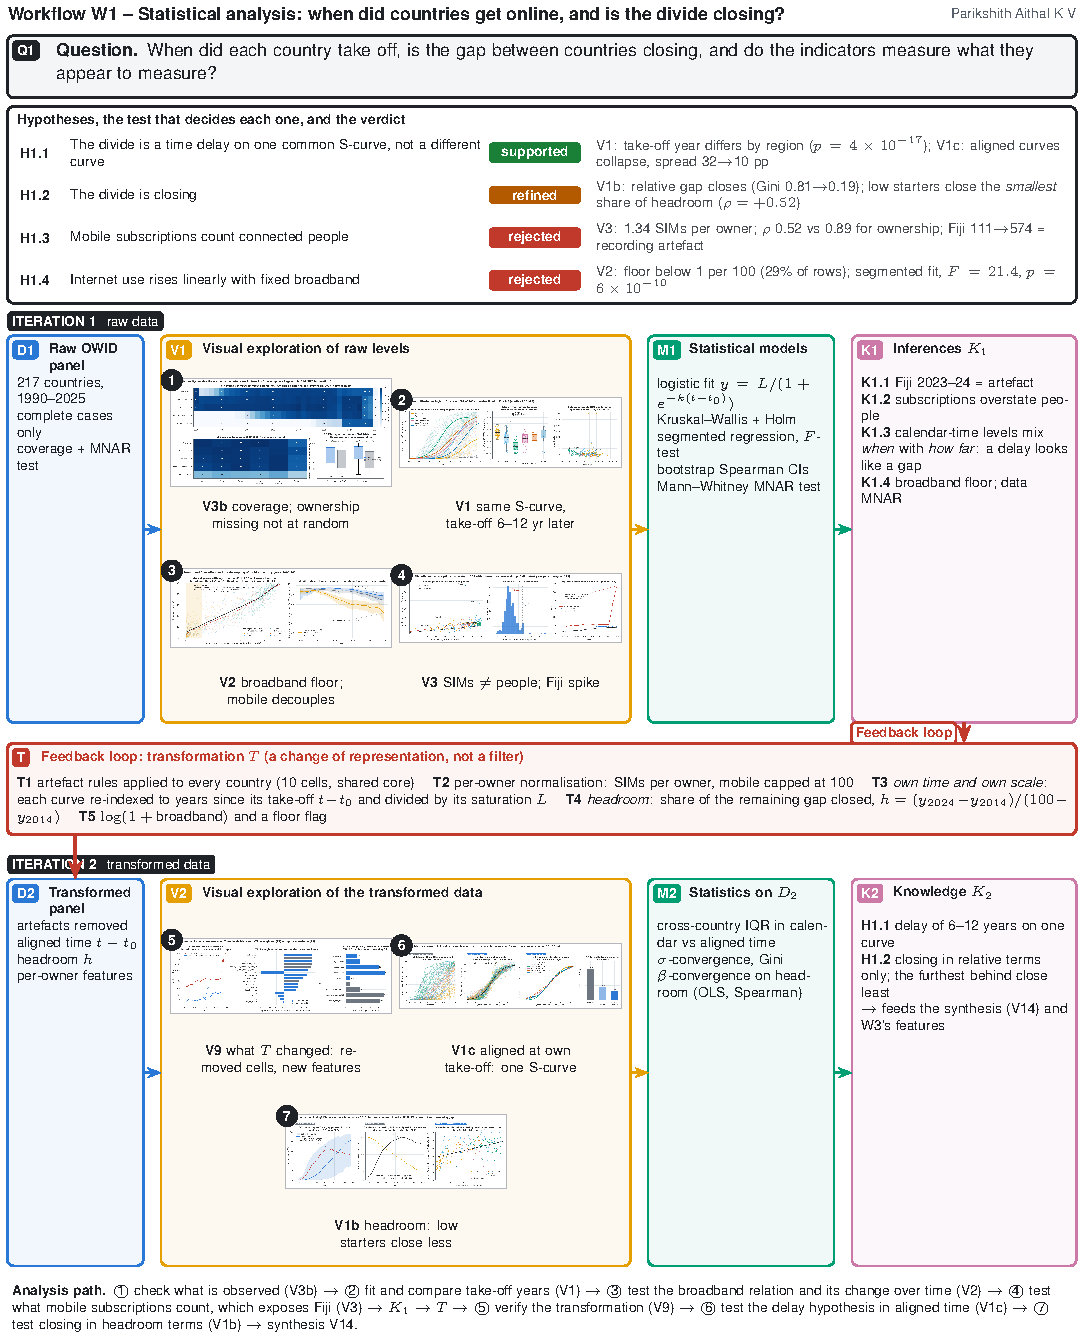
\includegraphics[width=\textwidth,height=0.92\textheight,keepaspectratio]{W1_workflow_statistics.pdf}
\caption{\textbf{Workflow W1, statistical analysis, unrolled.} Question and hypotheses with their
verdicts (top); iteration~1 on raw data with the four figures that produced $K_1$; the feedback loop
$T$, which re-expresses every series in its own time and scale and in headroom; iteration~2 on the
transformed data; the numbered analysis path (bottom).}
\label{fig:w1}
\end{figure*}

\hyp{Q1.}{When did each country take off, is the gap between countries closing, and do the indicators
measure what they appear to measure?}
Five hypotheses are tested (Fig.~\ref{fig:w1}): H1.1 the divide is a time delay on one common S-curve;
H1.2 the divide is closing; H1.3 mobile subscriptions count connected people; H1.4 internet use rises
linearly with fixed broadband; and H1.5, A1's own conclusion stated as a test, countries that leapfrogged
landlines with mobile caught up online.

\subsection{Iteration 1: raw levels in calendar time}
\textit{Diffusion is an S-curve shifted by region (Fig.~\ref{fig:v1}).} The logistic model fits 201
of 203 countries with $R^2\ge0.9$ (median $R^2=0.990$). The take-off year differs by region
(Kruskal--Wallis $H=86.3$, $p=4\times10^{-17}$). Africa's median take-off is 2017.5, 11.9 years after
Europe's 2005.6 (Mann--Whitney, Holm-corrected $p=1.4\times10^{-15}$); the other regions lag by
6.3--11.5 years. Take-off year and growth rate are weakly negatively correlated (Spearman
$\rho=-0.21$, $p=0.003$).

\inference{Take-off differs by up to 12 years, and late starters do not climb faster. Whether the
curves differ only by this delay cannot be read from calendar-time plots, in which timing and level
are mixed; this motivates T3.}

\begin{figure*}[!t]
\centering
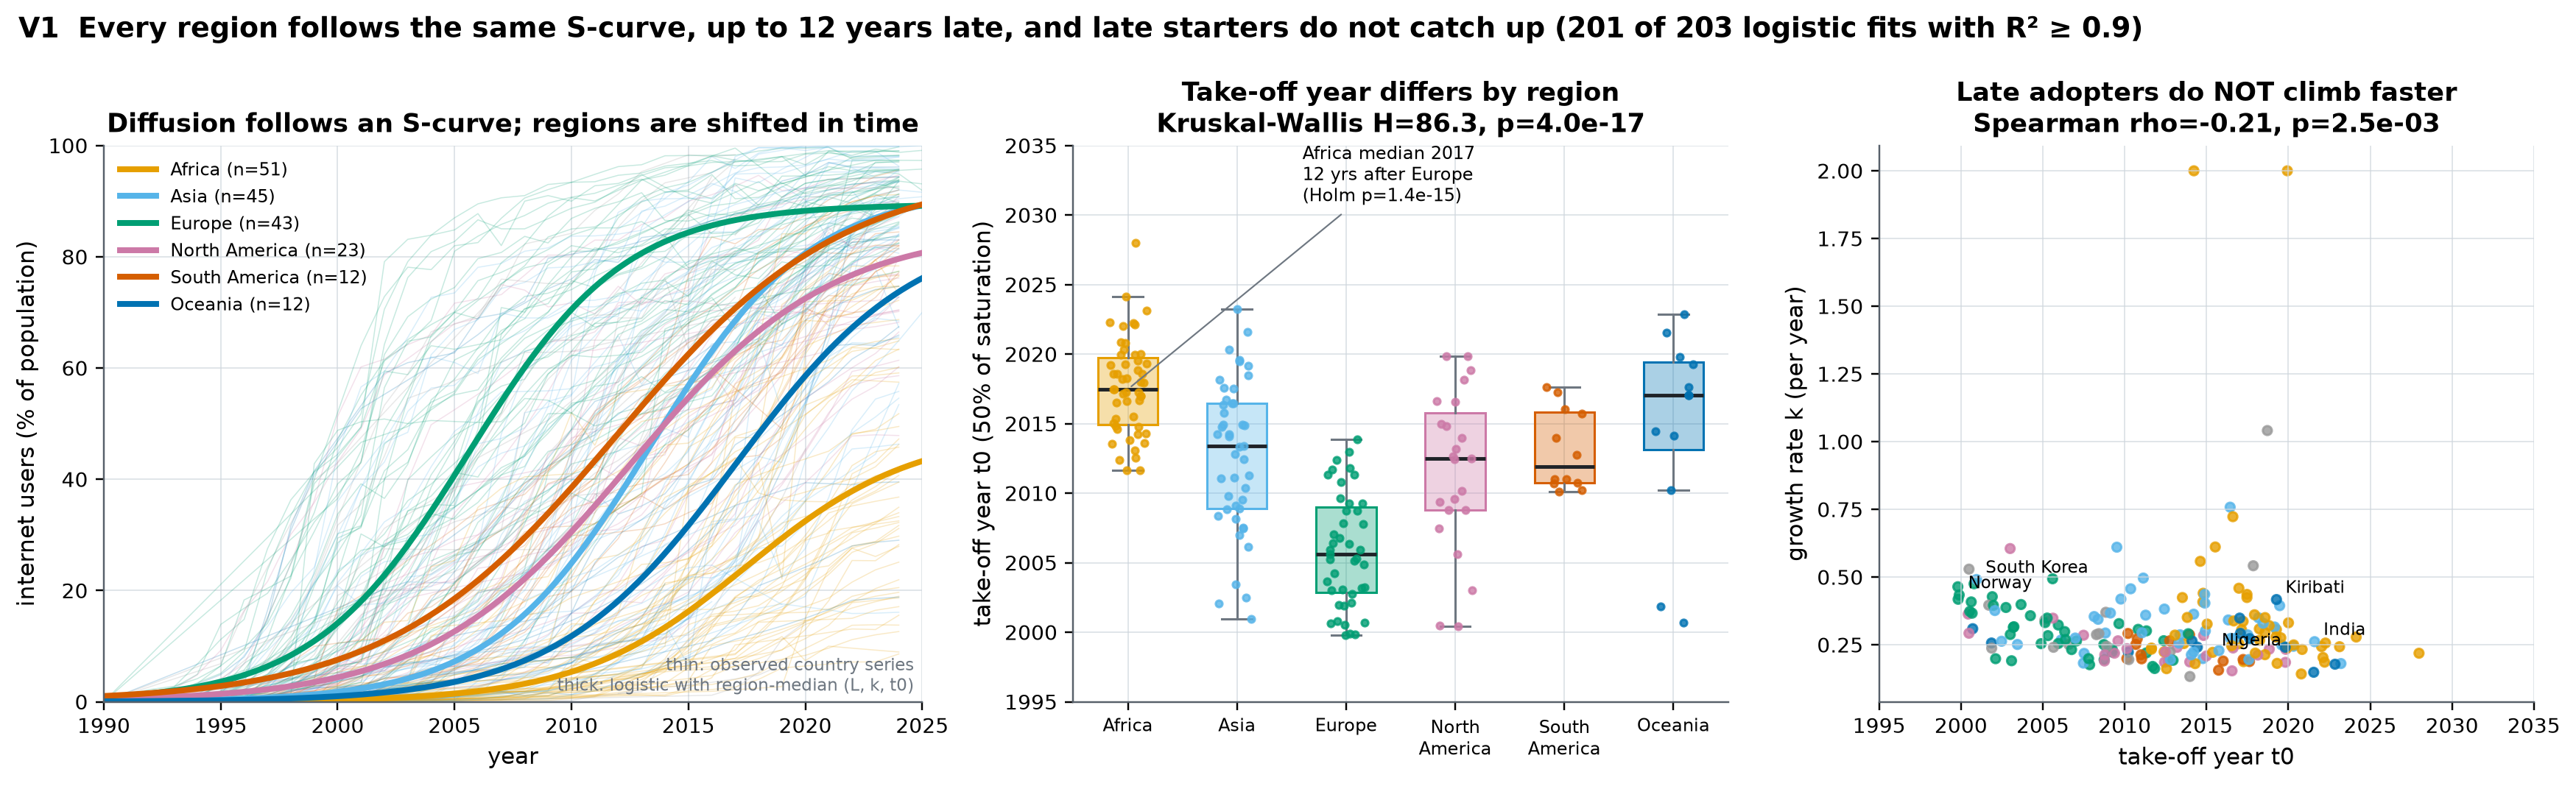
\includegraphics[width=\textwidth]{V1_diffusion_scurves.png}
\caption{\textbf{V1 (W1, step 1): every region follows an S-curve, shifted by up to 12 years, and late
adopters do not catch up faster.} Left: observed series (thin) and logistic curves with region-median
parameters (thick). Centre: take-off year by region with every country overplotted. Right: take-off
year against growth rate; two countries reach the $k\le2$ bound.}
\label{fig:v1}
\end{figure*}

\textit{Where the delay lies (Fig.~\ref{fig:v1d}).} Mapped, the take-off year forms contiguous areas
rather than scattered outliers: North America's two large economies, Western and Northern Europe,
Japan, South Korea and Australia took off by about 2005; South America, Russia and China around
2008--2012; and most of sub-Saharan Africa, South Asia and Indonesia after 2015. The regional medians
are 2006 for Europe, 2012 for North and South America (North America here includes Central America and
the Caribbean), 2013 for Asia and 2017 for Africa and Oceania.

\inference{The delay is geographic, so regions are a meaningful unit for the later tests, and any
calendar-time comparison mixes a country's position with the year it started; this strengthens the
case for T3.}

\begin{figure*}[!t]
\centering
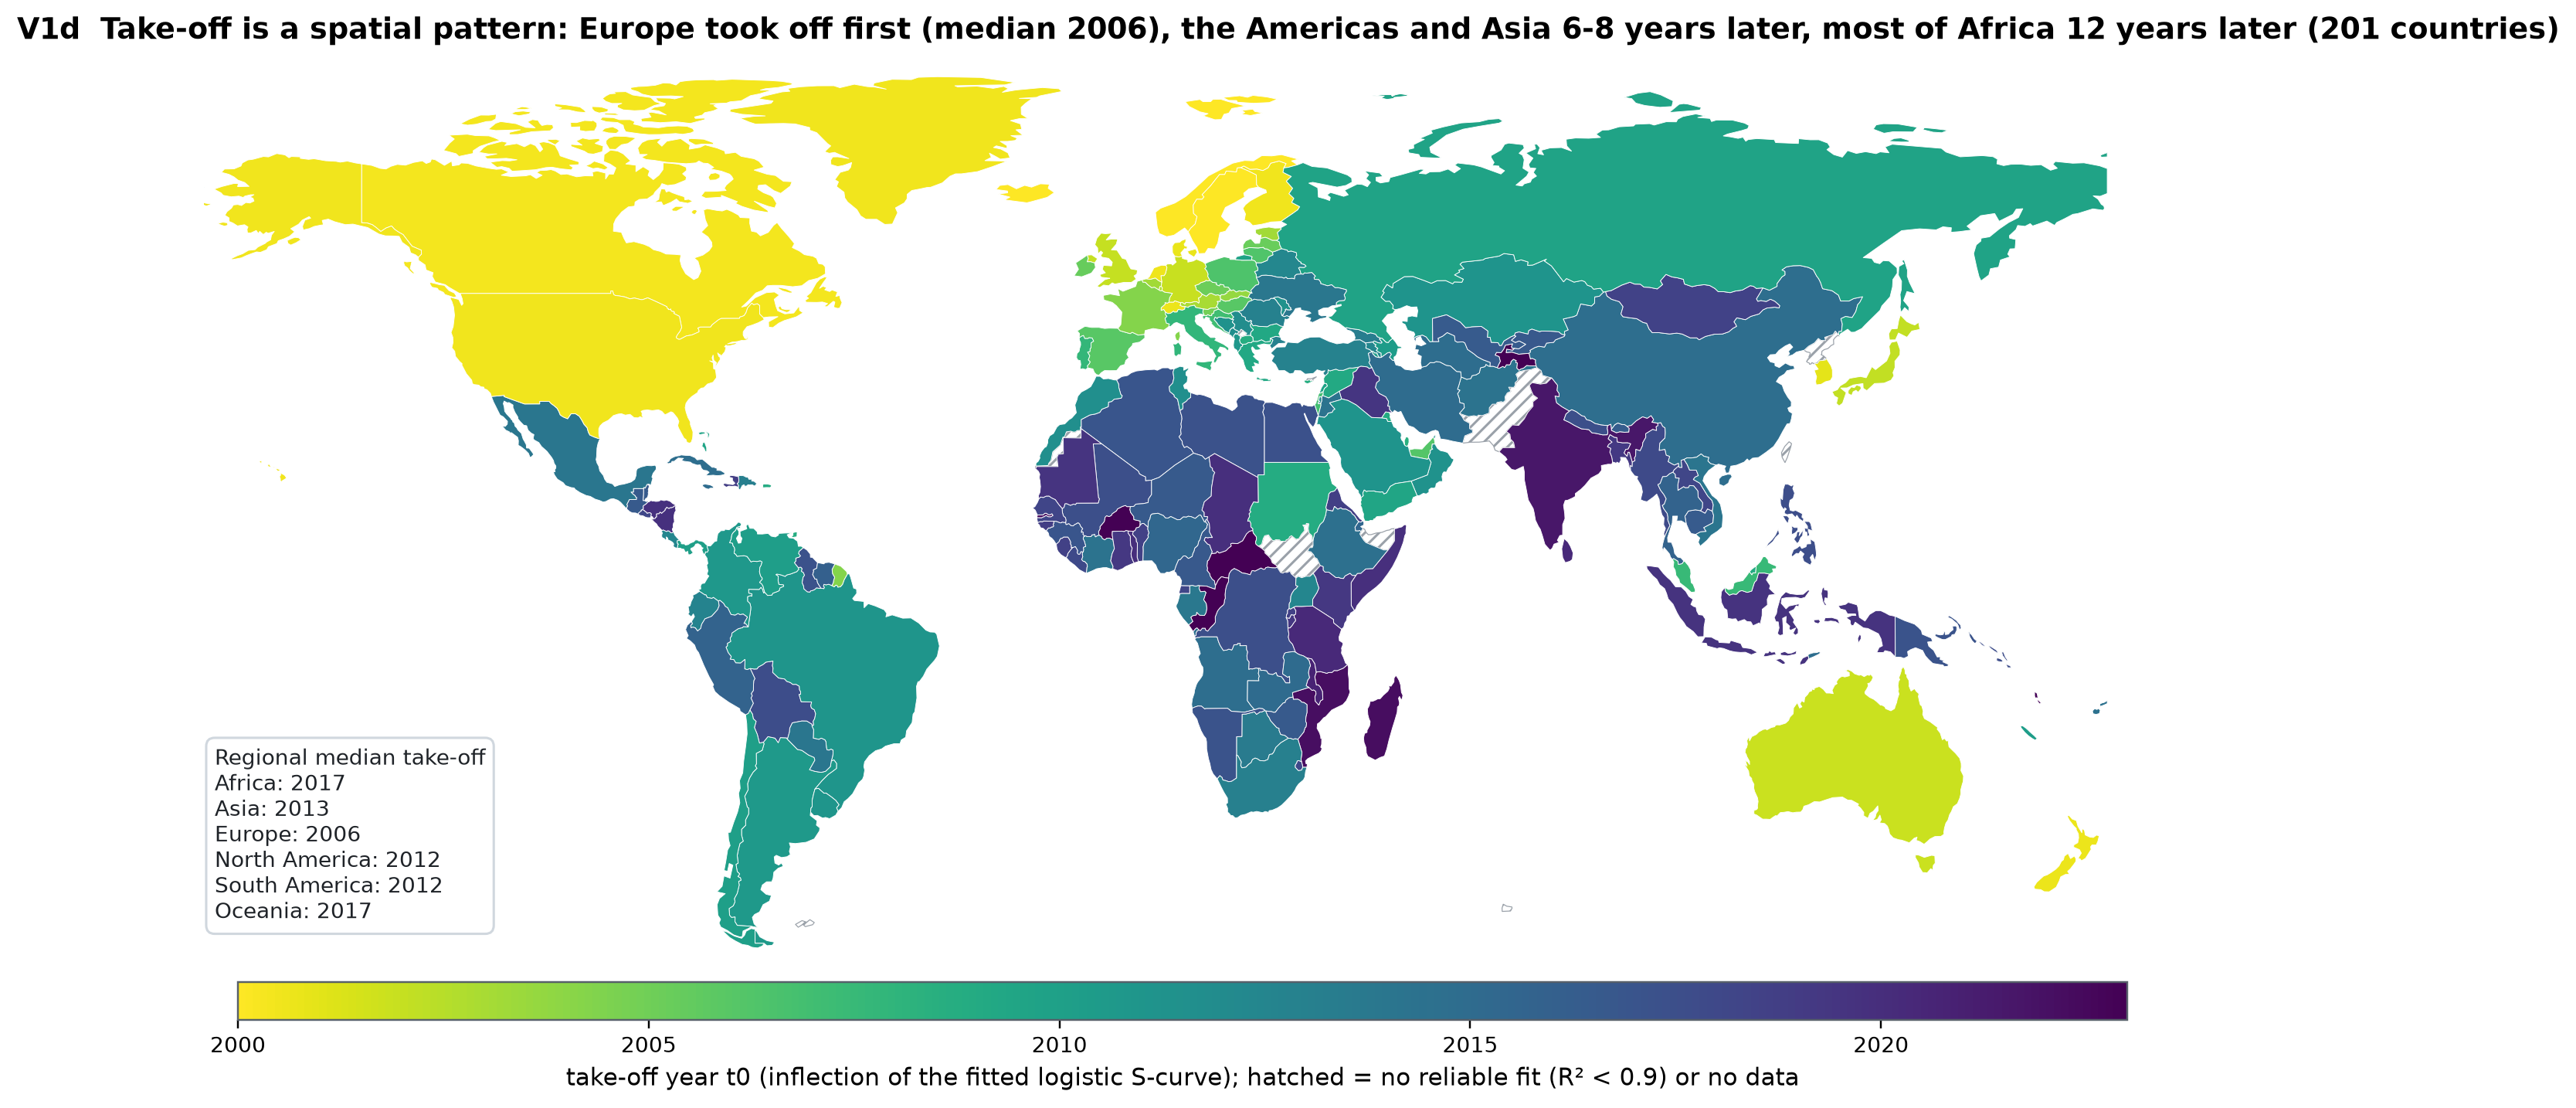
\includegraphics[width=\textwidth]{V1d_takeoff_map.png}
\caption{\textbf{V1d (W1, step 2): take-off is a spatial pattern, with most of Africa 12 years behind
Europe.} Take-off year $t_0$ of each country's logistic fit on a sequential, colour-blind-safe scale;
hatched countries have no reliable fit ($R^2<0.9$) or no data. The box lists regional medians.}
\label{fig:v1d}
\end{figure*}

\textit{A broadband floor and the decoupling of mobile (Fig.~\ref{fig:v2}).} Of 3{,}629
country-years in 2005--2024, 28.7\% have fewer than one broadband subscription per 100, yet internet
use on this floor reaches 30\% (median 9\%, 90th percentile 30\%). Above the floor, internet use rises
roughly linearly in $\log(1+\text{broadband})$; the segmented regression places a breakpoint near 23
per 100, where the slope steepens from 19.6 to 30.8 points per log-unit ($R^2=0.78$; $F=21.4$ against
a single line, $p=6\times10^{-10}$). In 2005 broadband, mobile and landlines all correlated at
$\rho\approx0.9$ with internet use, whereas by 2024 mobile had fallen to $\rho=0.42$ (95\% CI
0.26--0.57) and broadband held at 0.80 (0.71--0.87).

\inference{H1.4 is rejected: broadband acts non-linearly and has a floor below which it carries no
information. Mobile subscriptions stopped distinguishing countries once they saturated, so A1's
pooled correlation hid a trend over time.}

\begin{figure*}[!t]
\centering
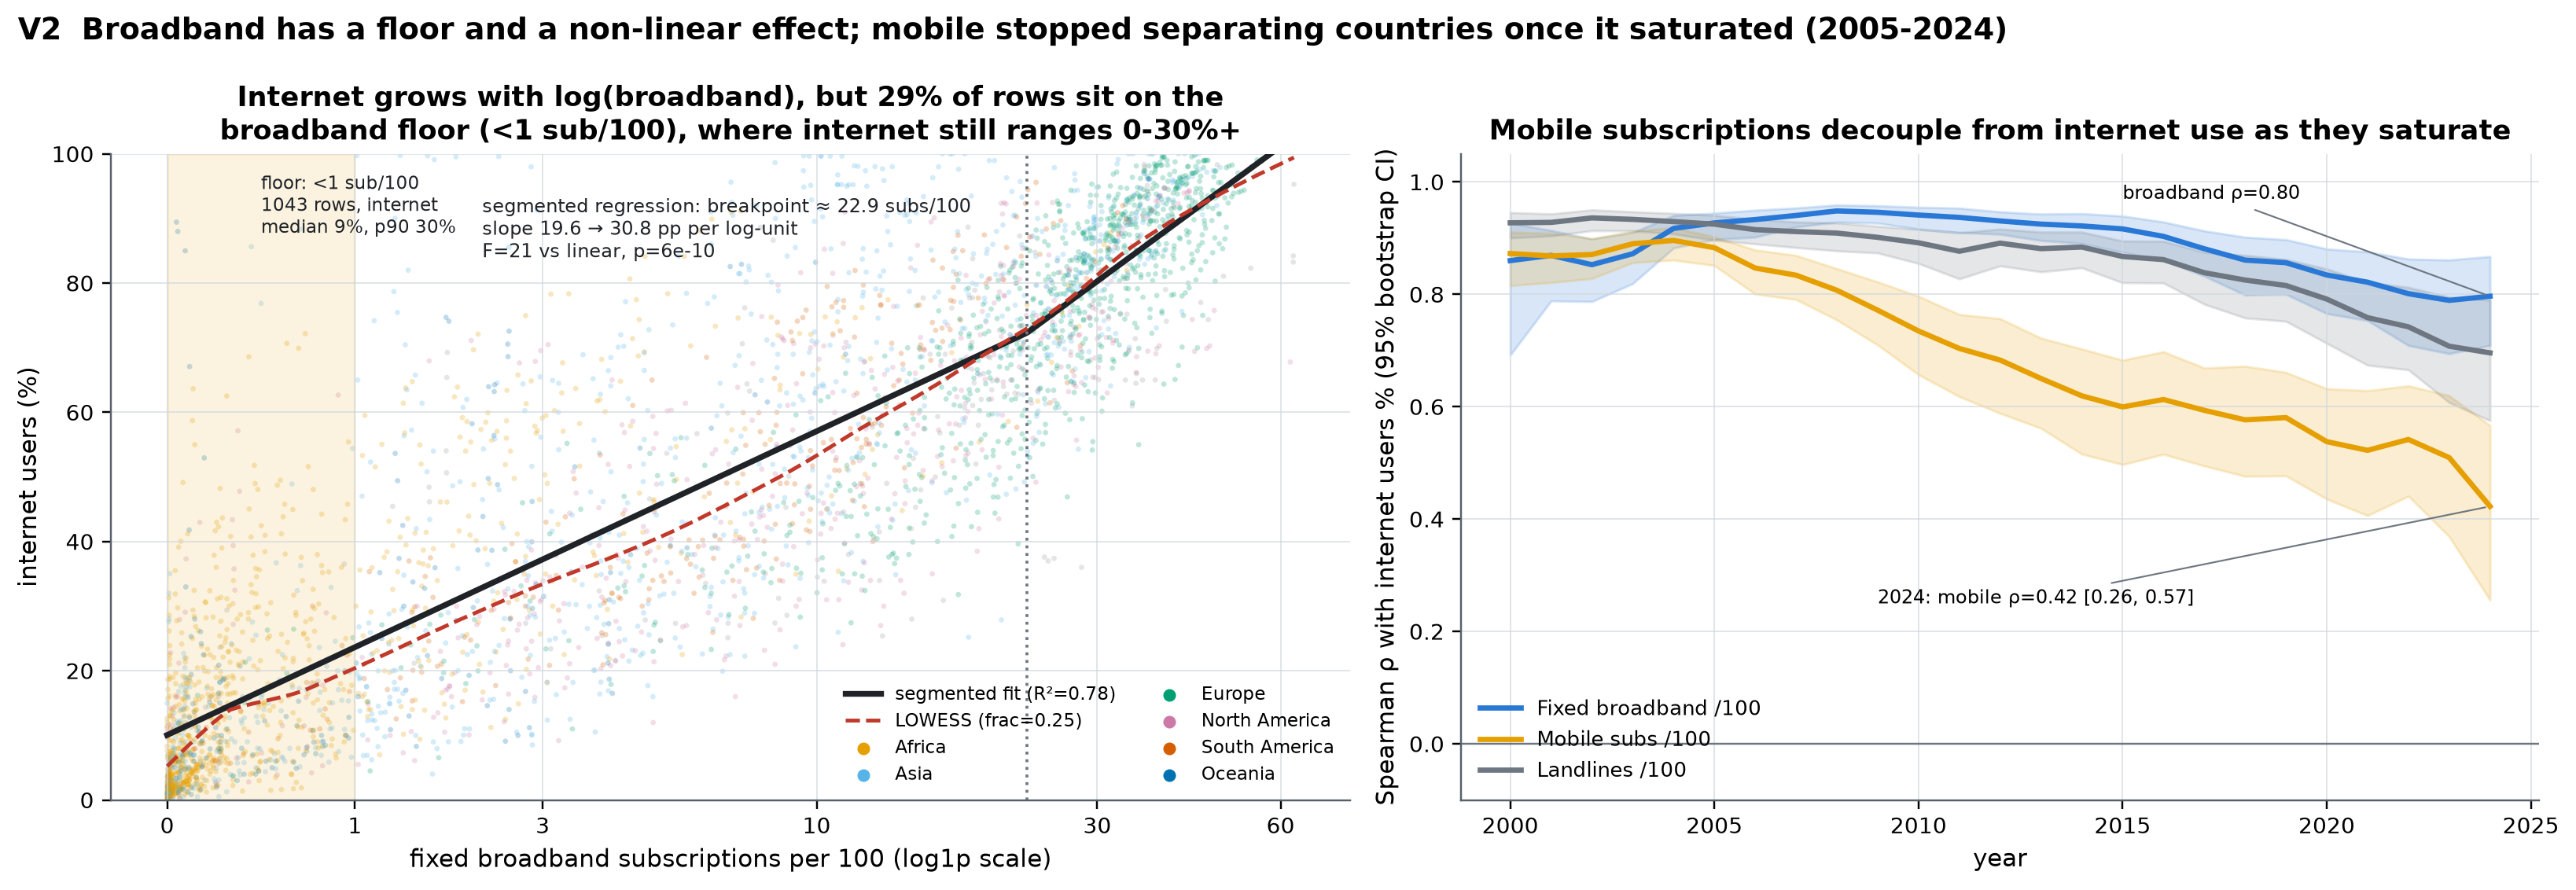
\includegraphics[width=\textwidth]{V2_floor_effect_decoupling.png}
\caption{\textbf{V2 (W1, step 3): broadband has a floor and a non-linear effect, and mobile lost its
power to separate countries after 2005.} Left: internet use against broadband (log1p axis) with a
segmented fit and LOWESS; the shaded band is the floor below one subscription per 100. Right: Spearman
$\rho$ with internet use by year, with 95\% country-bootstrap intervals.}
\label{fig:v2}
\end{figure*}

\textit{Subscriptions count SIMs, not people (Fig.~\ref{fig:v3}).} In each country's latest year
with both values ($n=193$), the median country has 1.34 SIMs per phone owner (IQR 1.15--1.61).
Ownership correlates at $\rho=0.89$ with internet use and subscriptions at only $\rho=0.52$. One
multi-SIM flag of 1.5 SIMs per owner is used throughout; it lies inside the upper quartile but below
the Tukey fence of 2.30, so it marks a market pattern (35\% of countries) rather than an outlier.
Fiji lies far outside every other country, at 574 subscriptions per 100 in 2024 with ownership
unchanged at 82\%.

\inference{H1.3 is rejected: raw subscriptions overstate people and must be normalised before
modelling. Fiji's jump from 111 to 574 in two years, with flat ownership and internet use, is a
recording artefact rather than adoption; W2 reaches the same conclusion independently (V6b).}

\begin{figure*}[!t]
\centering
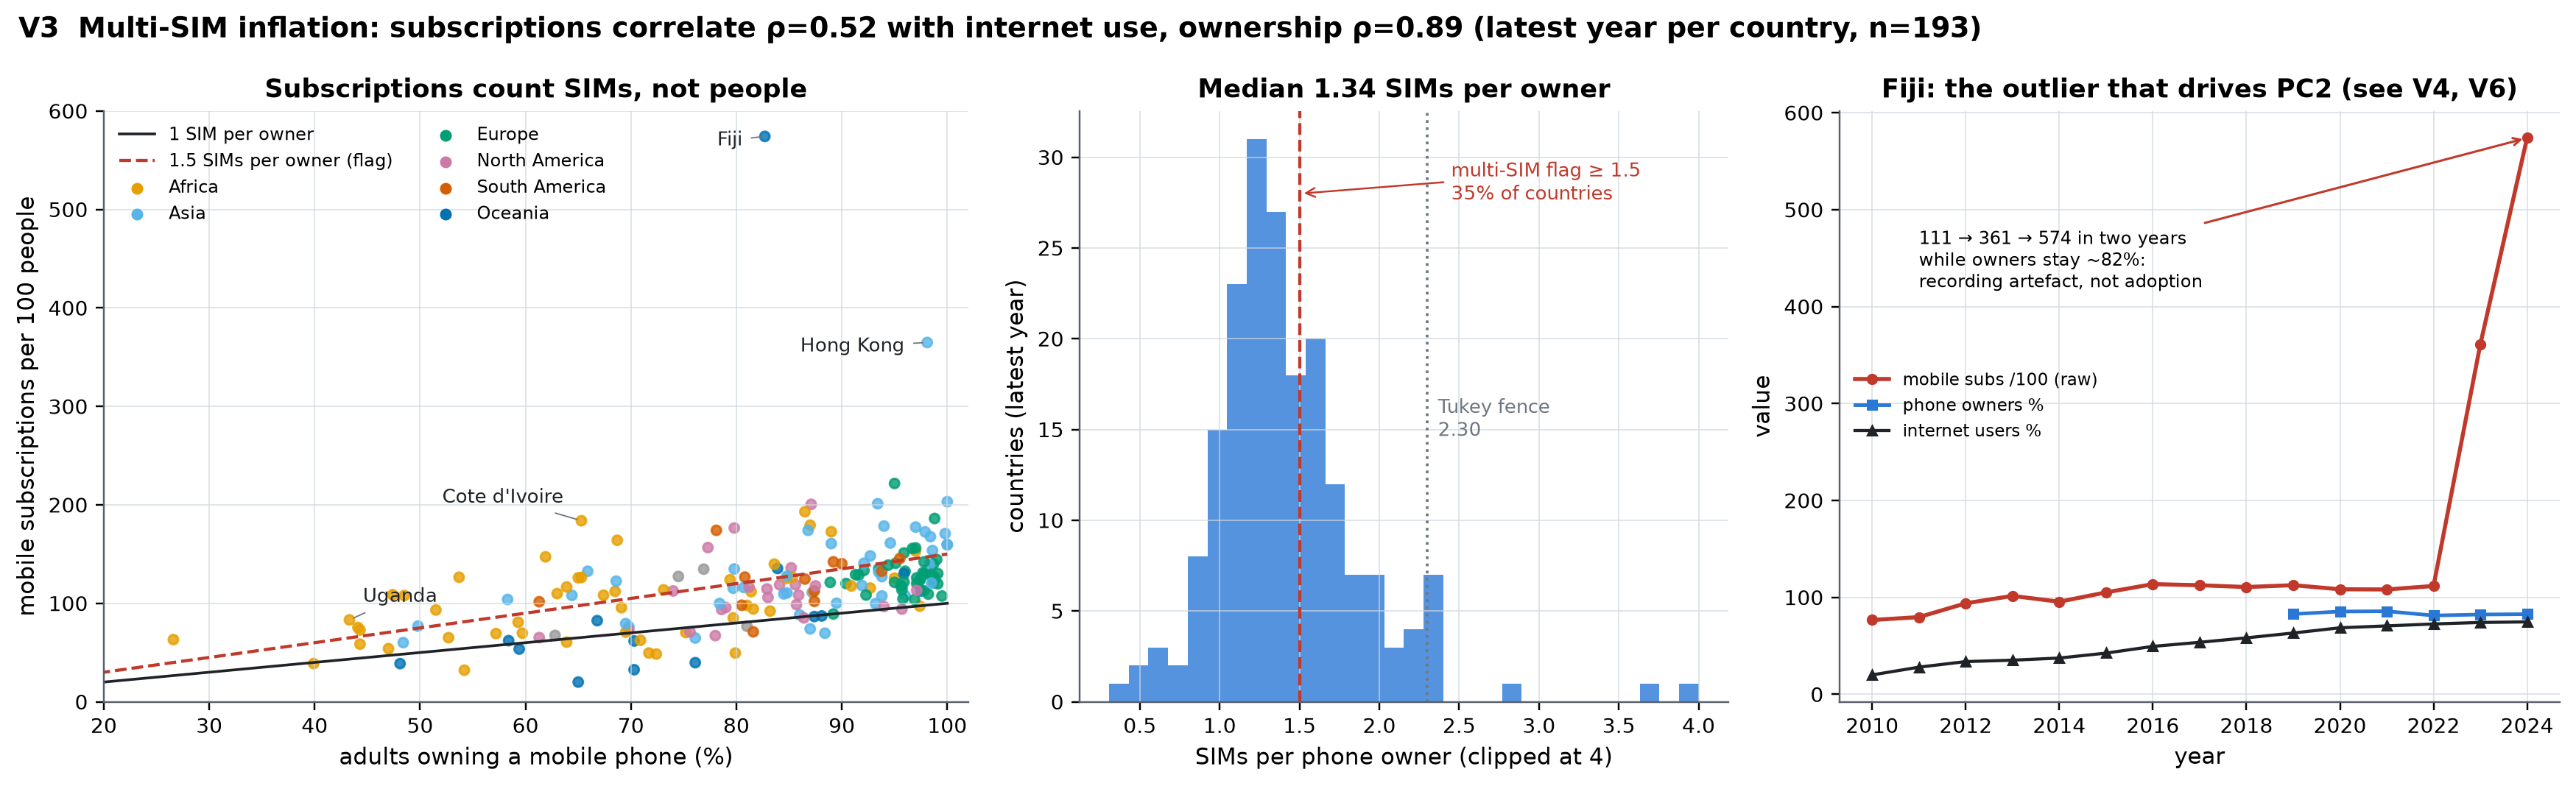
\includegraphics[width=\textwidth]{V3_multisim_inflation.png}
\caption{\textbf{V3 (W1, step 4): subscriptions overstate people by a median 1.34 SIMs per owner, and
Fiji's 2023--24 values are an artefact.} Left: subscriptions against ownership with one and 1.5
SIMs-per-owner lines. Centre: distribution of SIMs per owner with the team threshold and Tukey fence.
Right: Fiji's mobile series against ownership and internet use.}
\label{fig:v3}
\end{figure*}

\textit{Is the divide closing in raw terms? (Fig.~\ref{fig:v1e}a).} Relative inequality between
countries fell steadily: the Gini coefficient of internet shares dropped from 0.81 in 1995 to 0.19 in
2024. Absolute spread did not: the cross-country standard deviation rose until 2013 (29.3 points) and
has fallen only since, and the gap between the median European and the median African country peaked
at 64 points in 2014 and was still 52 in 2024.

\inference{The two raw measures disagree, because a measure on levels bounded at 100\% cannot separate
catching up from saturating. H1.2 needs a measure of the gap each country still has; this motivates
T4.}

\subsection{Inferences $K_1$ and the feedback loop}
Four inferences leave iteration~1 (W1 rows of Table~\ref{tab:loops}): Fiji's 2023--24 values are an
artefact (K1.1), subscriptions overstate people (K1.2), calendar-time levels mix when a country started
with how far it has come (K1.3), and broadband has a floor while the data are missing not at random
(K1.4). They become five transformations. T1 removes artefacts by rule from every country; T2 changes
the measurement scale of mobile; T3 changes the coordinate system of every series to its own time and
scale; T4 replaces levels by headroom; and T5 re-expresses broadband and defines the floor and
missingness flags that W3 uses. Fig.~\ref{fig:v9} is the first view of iteration~2 and verifies what
$T$ changed: of the ten removed cells, two are Fiji's level shift (rule A) and eight are isolated
one-year spikes (rule B) in broadband (six), landlines (one) and internet use (one), each listed in the
artefact log. Pooled correlations are inflated by the shared time trend (raw mobile reaches 0.89
pooled against 0.42 within 2024), so the engineered features are read for new information rather than
size: \texttt{broadband\_zero} isolates the floor ($-0.74$), and the history features
(\texttt{landline\_decline} 0.74, \texttt{years\_since\_mobile\_gt\_landline} 0.75) carry information
that no single-year value has.

\begin{figure*}[!t]
\centering
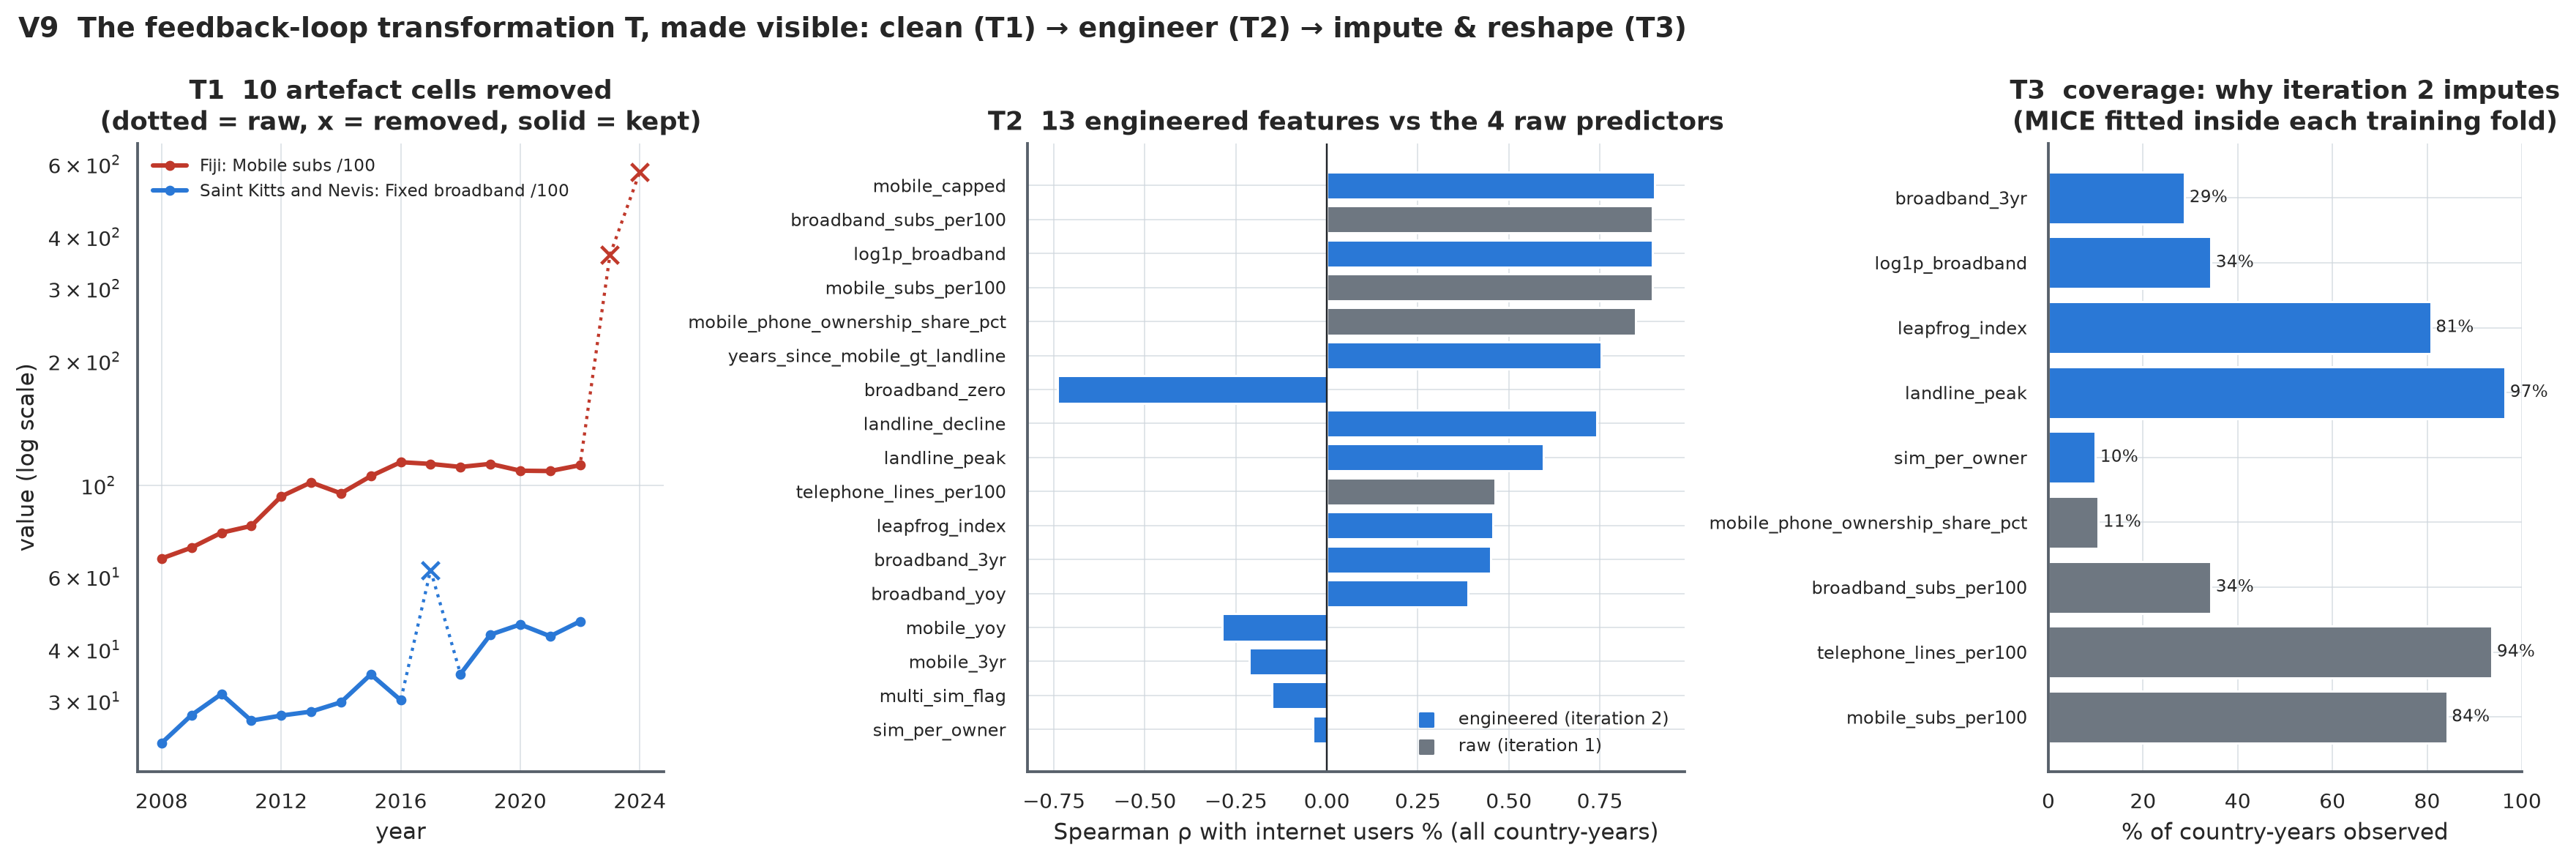
\includegraphics[width=\textwidth]{V9_feedback_transformation.png}
\caption{\textbf{V9 (W1, step 5): the transformation removes ten artefact cells and adds features that
no single-year value contains.} T1: artefact removal (crosses mark removed cells). T2: Spearman $\rho$
of engineered (blue) and raw (grey) features with internet use. T3: coverage of raw and engineered
features.}
\label{fig:v9}
\end{figure*}

\subsection{Iteration 2: own time, own scale, headroom and the leapfrog test}
\textit{Delay, not difference (Fig.~\ref{fig:v1c}).} In calendar years the 201 well-fitted curves
spread over two decades, and the mean cross-country IQR is 32.0 points. Re-indexed to each country's
own take-off year the IQR falls to 13.6, and divided also by each country's saturation level it falls
to 9.7, a 3.3-fold reduction. The decisive panel is (c): the six regional median curves, whose take-off
years range from 2006 (Europe) to 2017 (Africa and Oceania), lie on top of each other and on one
logistic curve with the median growth rate $k=0.27$. Because $t_0$ and $L$ are fitted to the same
curves, some collapse is expected for any good fit; what the figure adds is that one \emph{shape} serves
every region, so the regional differences of V1 are differences of timing only.

\begin{figure*}[!t]
\centering
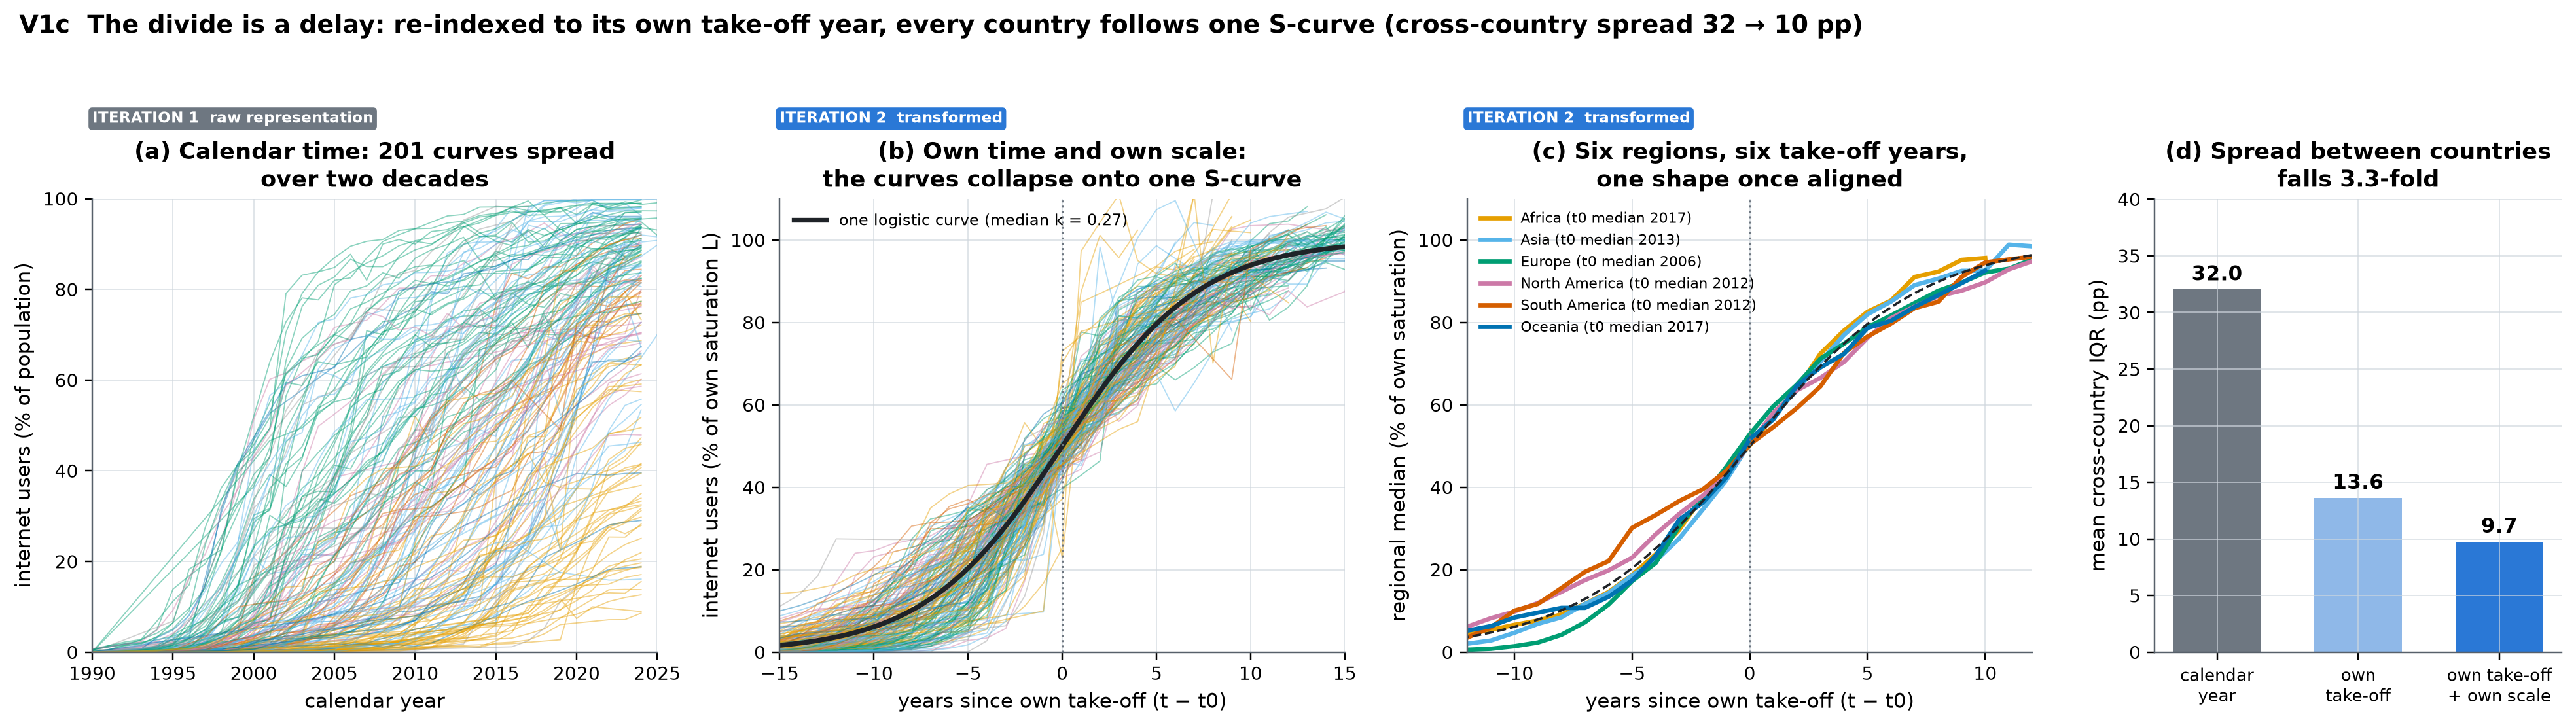
\includegraphics[width=\textwidth]{V1c_takeoff_alignment.png}
\caption{\textbf{V1c (W1, step 6): re-indexed to its own take-off year and scaled to its own
saturation, every country follows one S-curve.} (a) Iteration~1 view: 201 curves in calendar time,
coloured by region. (b) Iteration~2 view: the same curves against years since take-off, as a share of
saturation, with one logistic curve. (c) Regional median curves after alignment. (d) Mean
cross-country IQR in the three representations.}
\label{fig:v1c}
\end{figure*}

\textit{Closing in headroom terms (Fig.~\ref{fig:v1e}b).} Between 2014 and 2024, countries that
started higher closed a \emph{larger} share of their remaining headroom (Spearman $\rho=+0.52$,
$p=10^{-13}$, 175 countries): 32 of 51 African countries closed less than 40\% of their gap, whereas
28 of 39 European countries closed more than 60\% (medians 32\% and 67\%).

\begin{figure*}[!t]
\centering
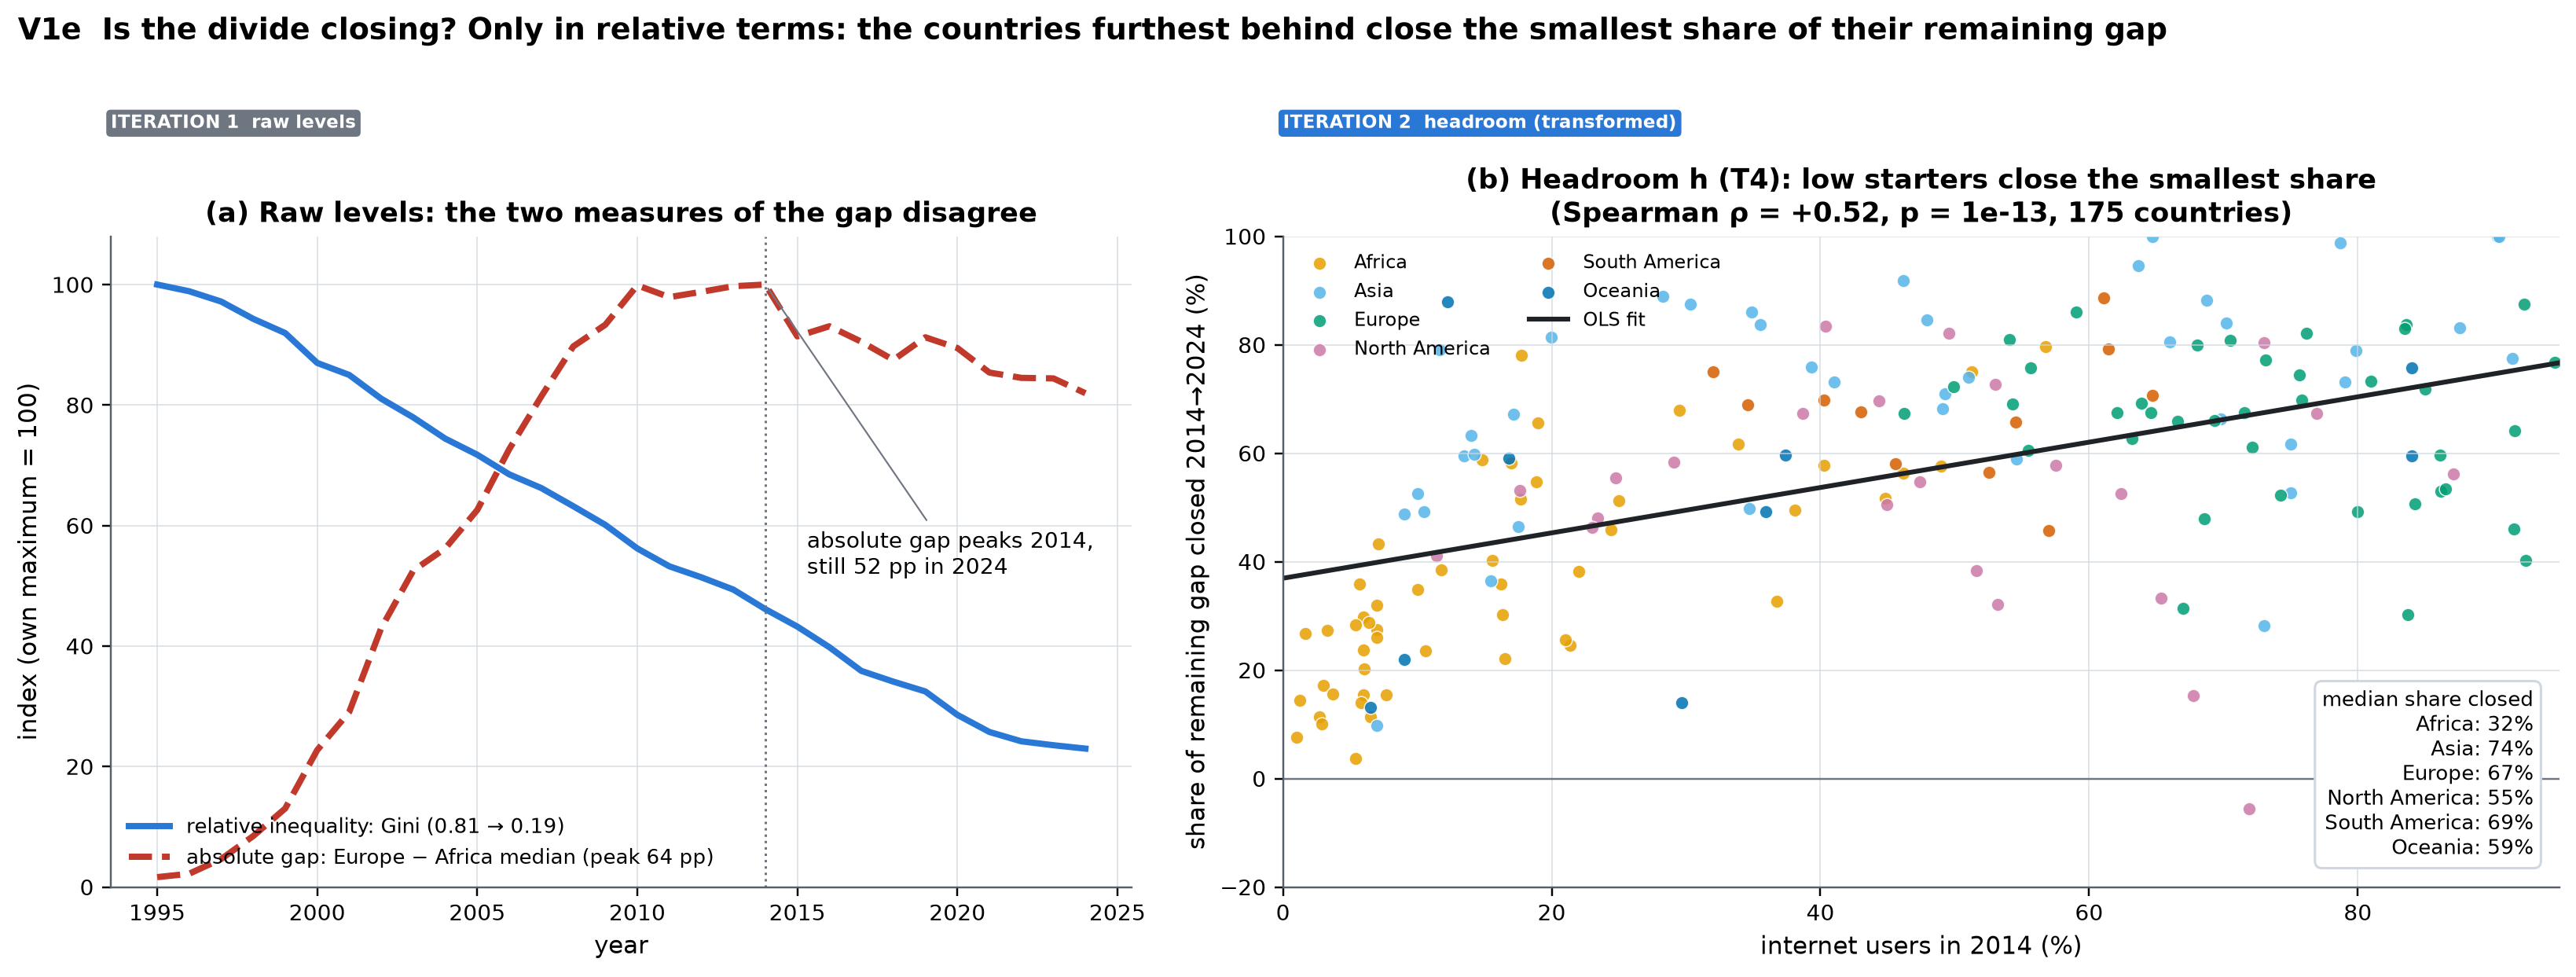
\includegraphics[width=\textwidth]{V1e_headroom_closing.png}
\caption{\textbf{V1e (W1, step 7): the divide is closing only in relative terms, and the countries
furthest behind close the smallest share of their remaining gap.} (a) Iteration~1, raw levels: Gini
coefficient and the Europe--Africa median gap, each indexed to its own maximum. (b) Iteration~2,
headroom (T4): share of the gap closed 2014--2024 against the 2014 level, with an OLS fit and
regional medians.}
\label{fig:v1e}
\end{figure*}

\textit{Did leapfrogging close the divide? (Fig.~\ref{fig:v1f}).} The engineered features of T2 allow
A1's conclusion to be tested directly. In 2024 ($n=143$ countries), the landline peak a country ever
reached correlates with internet use at $\rho=0.82$, and at 0.86 within Africa alone ($n=39$), whereas
capped mobile reaches only 0.47. Twenty-two countries never built landlines (peak below 5 per 100) yet
are saturated on mobile (capped at least 80 per 100); 17 of them are African. Their median internet use
is 44\%, against 93\% in the 73 countries whose landline peak exceeded 20 per 100 (Mann--Whitney
$p=10^{-11}$). The landline peak is not a cause: it also stands for the national investment and income
that built both networks, and no income variable is used (Section~\ref{sec:limits}).

\begin{figure*}[!t]
\centering
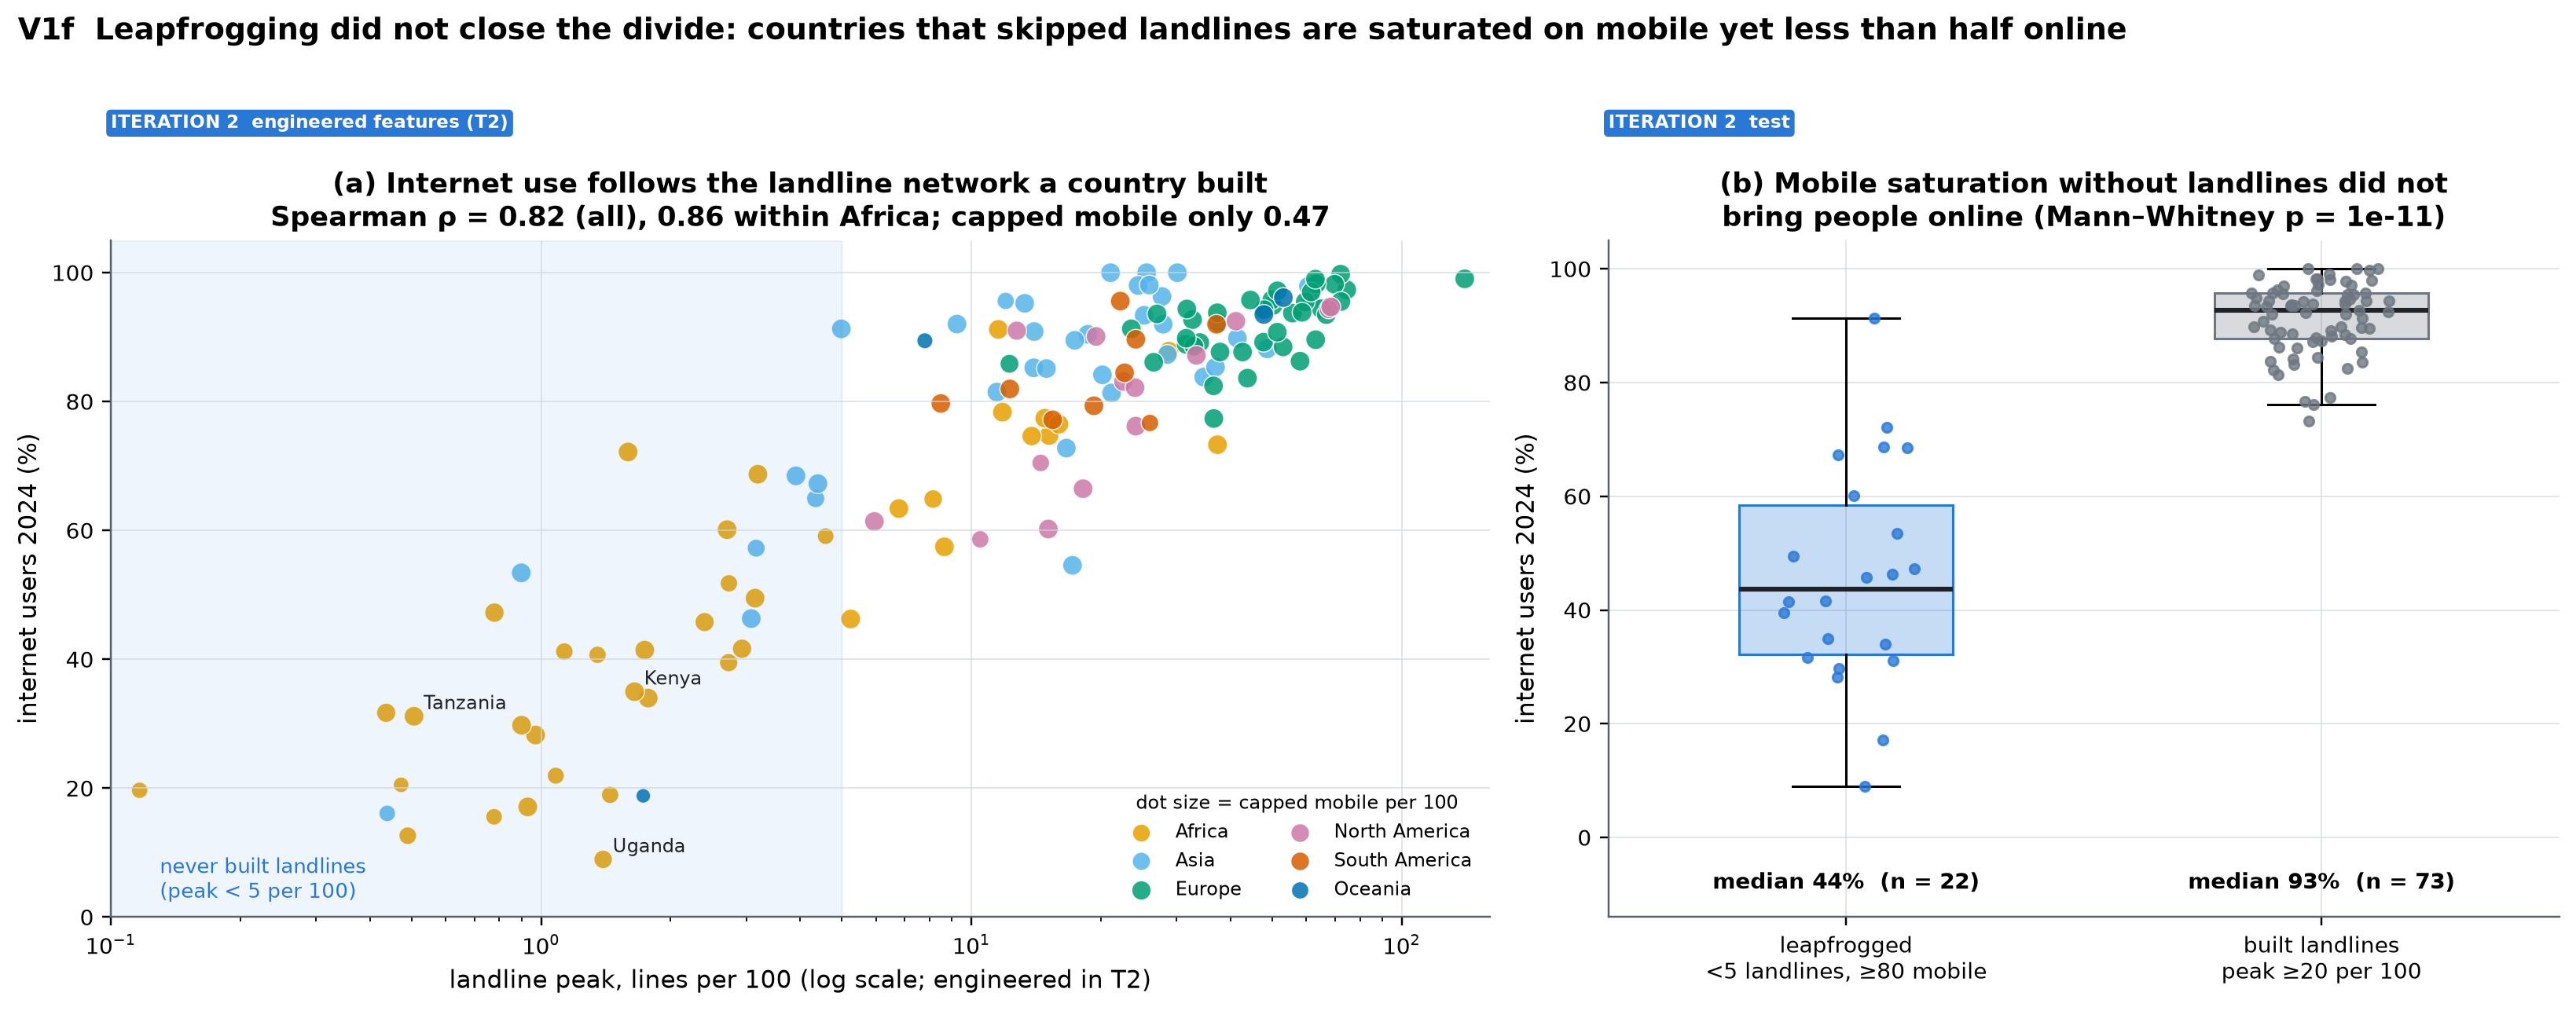
\includegraphics[width=\textwidth]{V1f_leapfrog_test.png}
\caption{\textbf{V1f (W1, step 8): leapfrogging did not close the divide.} (a) Internet use in 2024
against the landline peak (log scale), coloured by region and sized by capped mobile; the shaded band
marks countries that never built landlines. (b) Countries that leapfrogged (landline peak $<5$,
capped mobile $\ge80$ per 100) against countries that built landlines (peak $\ge20$), with every
country overplotted.}
\label{fig:v1f}
\end{figure*}

\subsection{Knowledge $K_2$ and the analysis path}
H1.1 is supported: the divide is a delay of 6--12 years on one common curve, as Comin and
Hobijn~\cite{comin2010} found for earlier technologies. H1.2 is refined: the divide is closing in
relative terms only, and the countries furthest behind close the smallest share of their gap, so there
is no $\beta$-convergence in headroom. H1.3 and H1.4 are rejected, and their rejection defines the
features that W3 uses. H1.5 is rejected: countries that skipped landlines reached mobile saturation
but not internet use, so leapfrogging happened without closing the divide.

\textit{Analysis path.} Coverage was checked first (coverage counts and the MNAR test) because every later test
depends on what is observed. The take-off fits (V1) raised the delay hypothesis and the map (V1d) showed that it is geographic; the broadband relation (V2) and the
measurement test (V3) followed because A1's evidence rested on these two indicators, and V3 exposed
Fiji. After the transformation, V9 verified it, V1c tested the delay hypothesis in aligned time,
V1e tested closing in headroom terms, and V1f tested leapfrogging directly with the engineered features. The result enters the synthesis (V14a).

% =========================================================================================
\section{Workflow W2: Unsupervised Mining}\label{sec:w2}
% =========================================================================================
\begin{figure*}[p]
\centering
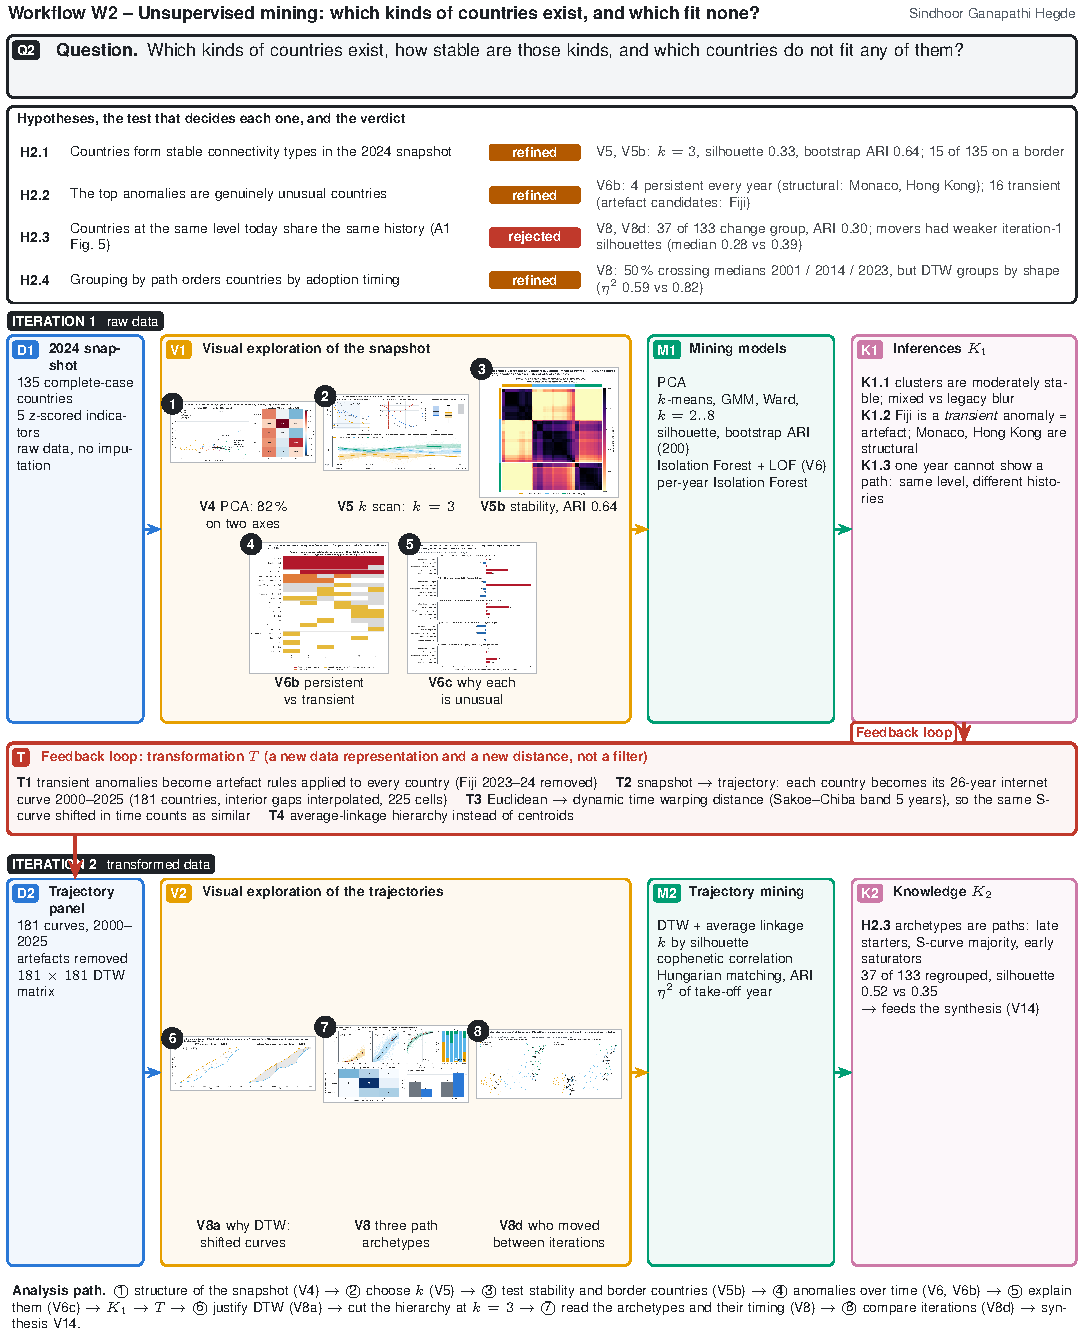
\includegraphics[width=\textwidth,height=0.92\textheight,keepaspectratio]{W2_workflow_unsupervised.pdf}
\caption{\textbf{Workflow W2, unsupervised mining, unrolled.} Question and hypotheses (top); iteration~1
on the 2024 snapshot with six of its seven figures; the feedback loop $T$, which turns snapshots into
trajectories under a time-shift-invariant distance; iteration~2 with five figures; the numbered
analysis path (bottom).}
\label{fig:w2}
\end{figure*}

\hyp{Q2.}{Which kinds of countries exist, how stable are those kinds, and which countries do not fit
any of them?}
Four hypotheses are tested (Fig.~\ref{fig:w2}): H2.1 countries form stable connectivity types in the
2024 snapshot; H2.2 the top anomalies are genuinely unusual countries; H2.3 countries at the same
level today share the same history (A1 Fig.~5); H2.4 grouping by path orders countries by adoption
timing.

\subsection{Iteration 1: the 2024 snapshot}
\textit{Structure (Fig.~\ref{fig:v4}).} On the 2024 snapshot (135 complete-case countries, five
z-scored indicators), PCA places 64.2\% of the variance on a general connectivity axis on which all
five indicators load positively, and 17.8\% on a second axis loaded almost entirely by mobile
subscriptions (0.96). Two countries, Fiji and Hong Kong, stretch the second axis on their own. The
third component (11\%) contrasts landlines with ownership and internet use, i.e.\ legacy fixed lines
that did not turn into internet use.

\begin{figure*}[!t]
\centering
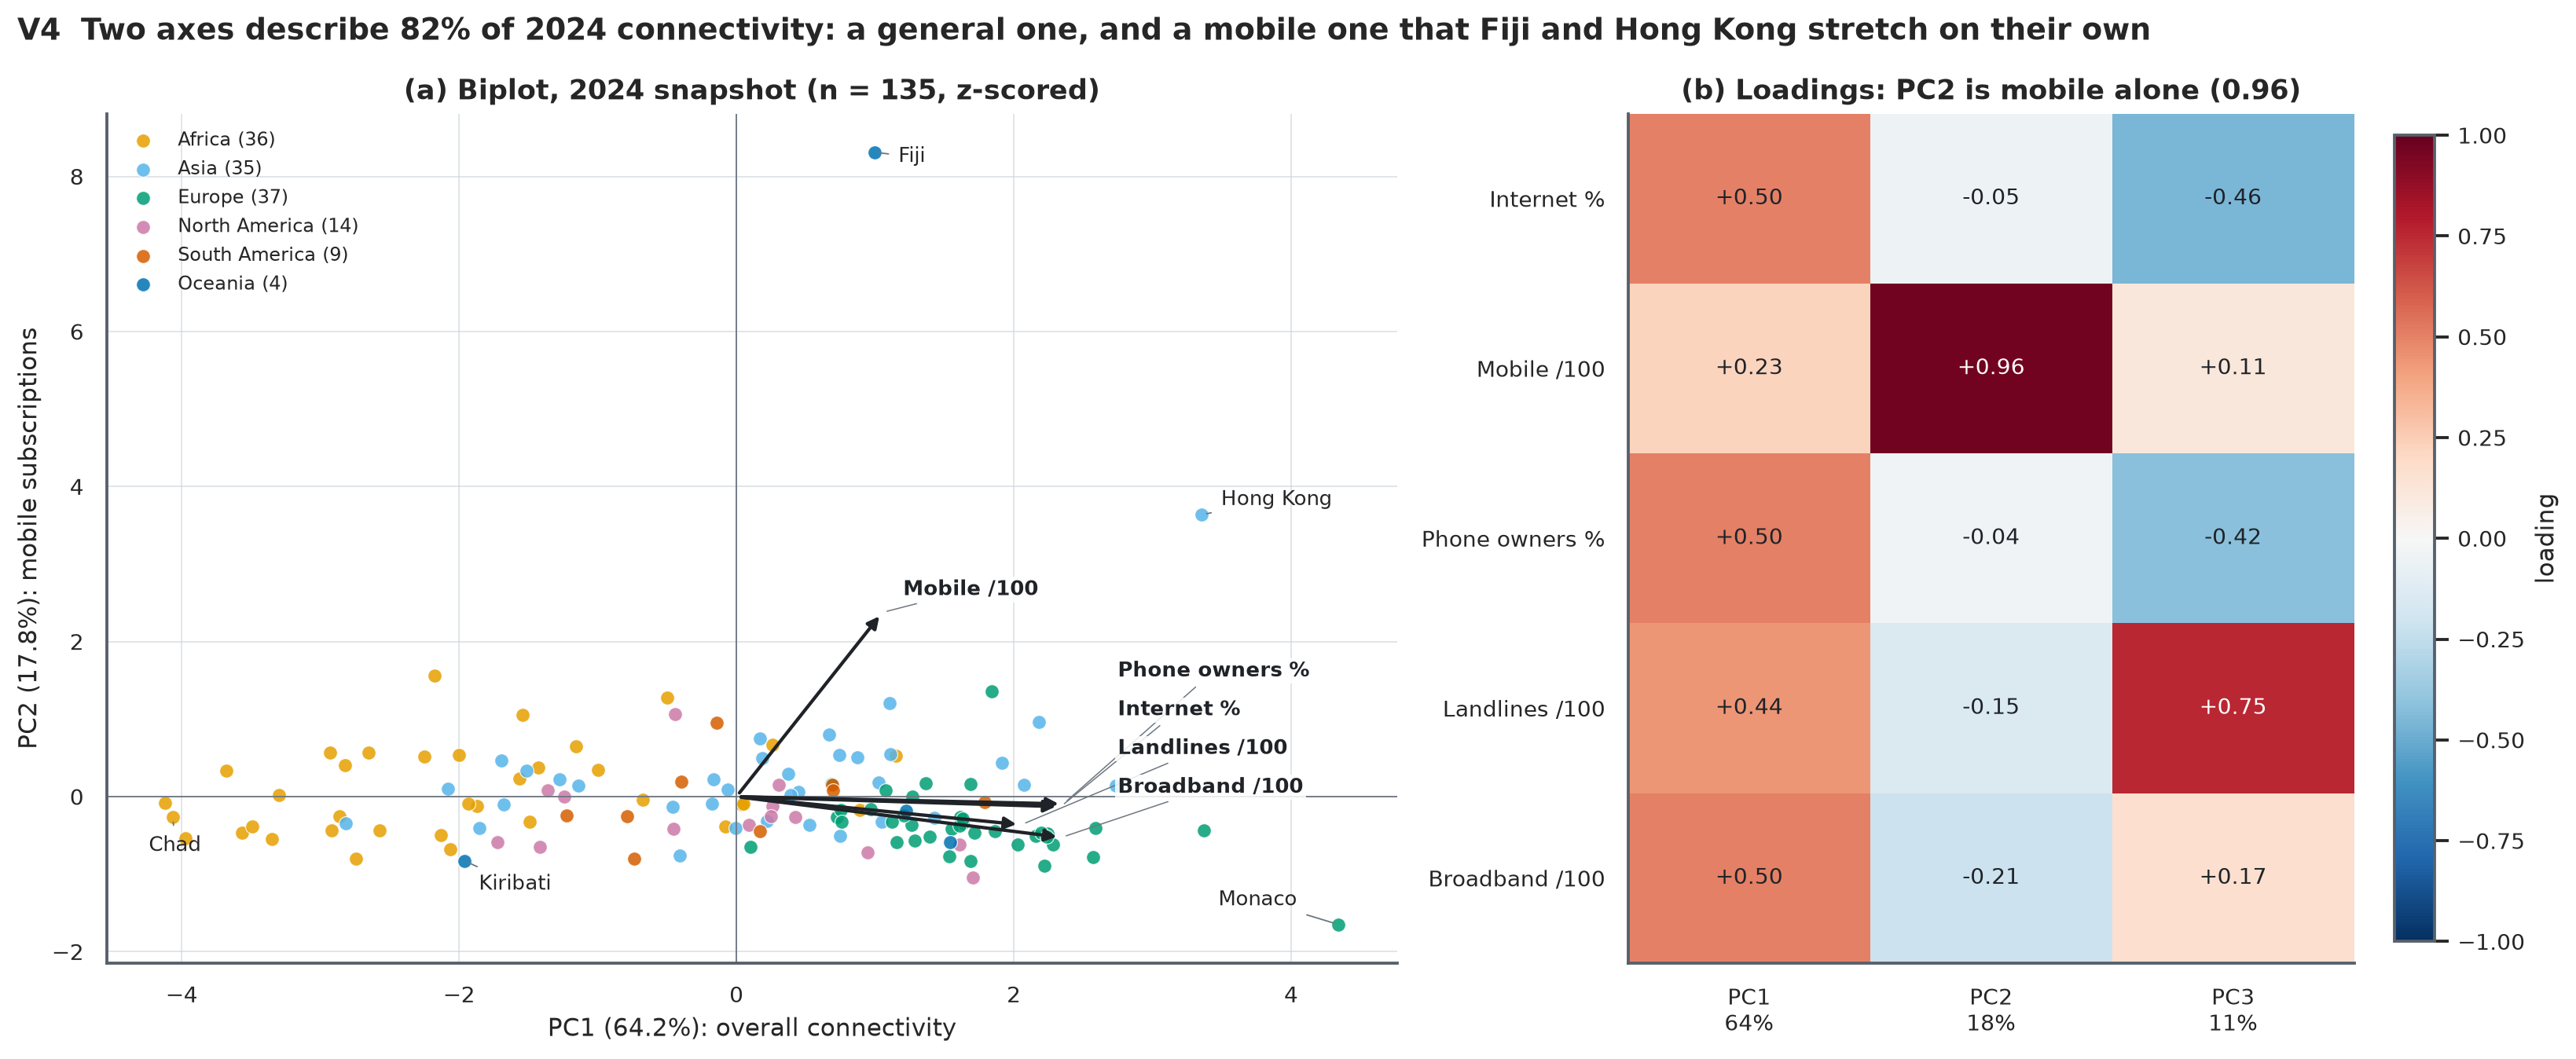
\includegraphics[width=\textwidth]{V4_pca_biplot.png}
\caption{\textbf{V4 (W2, step 1): two axes describe 82\% of 2024 connectivity, and the mobile axis is
driven by two countries.} (a) Biplot coloured by region with loading vectors. (b) Loadings of the
first three components.}
\label{fig:v4}
\end{figure*}

\textit{Choosing $k$ (Fig.~\ref{fig:v5}).} $k$ was scanned from 2 to 8 for $k$-means, GMM and Ward.
$k=2$ has the highest $k$-means silhouette (0.45) but only separates low from high; within
$k\in[3,6]$ and with no cluster smaller than four countries, $k=3$ maximises it (0.33). GMM's BIC is
lowest at $k=5$, but at $k\ge4$ the smallest $k$-means cluster holds only two countries, i.e.\
outliers rather than groups. The three $k$-means clusters order cleanly by connectivity, with median
internet use of 49, 88 and 94\%, landlines of 0.8, 10.8 and 30.1 and broadband of 1.5, 20.3 and 39.2
per 100: C0 mobile-first, C1 mixed and C2 fixed-line legacy, the groups of A1 Fig.~23. Ward's
apparently best silhouette (0.47) is an artefact, since one of its three clusters contains only Fiji
and Hong Kong.

\begin{figure*}[!t]
\centering
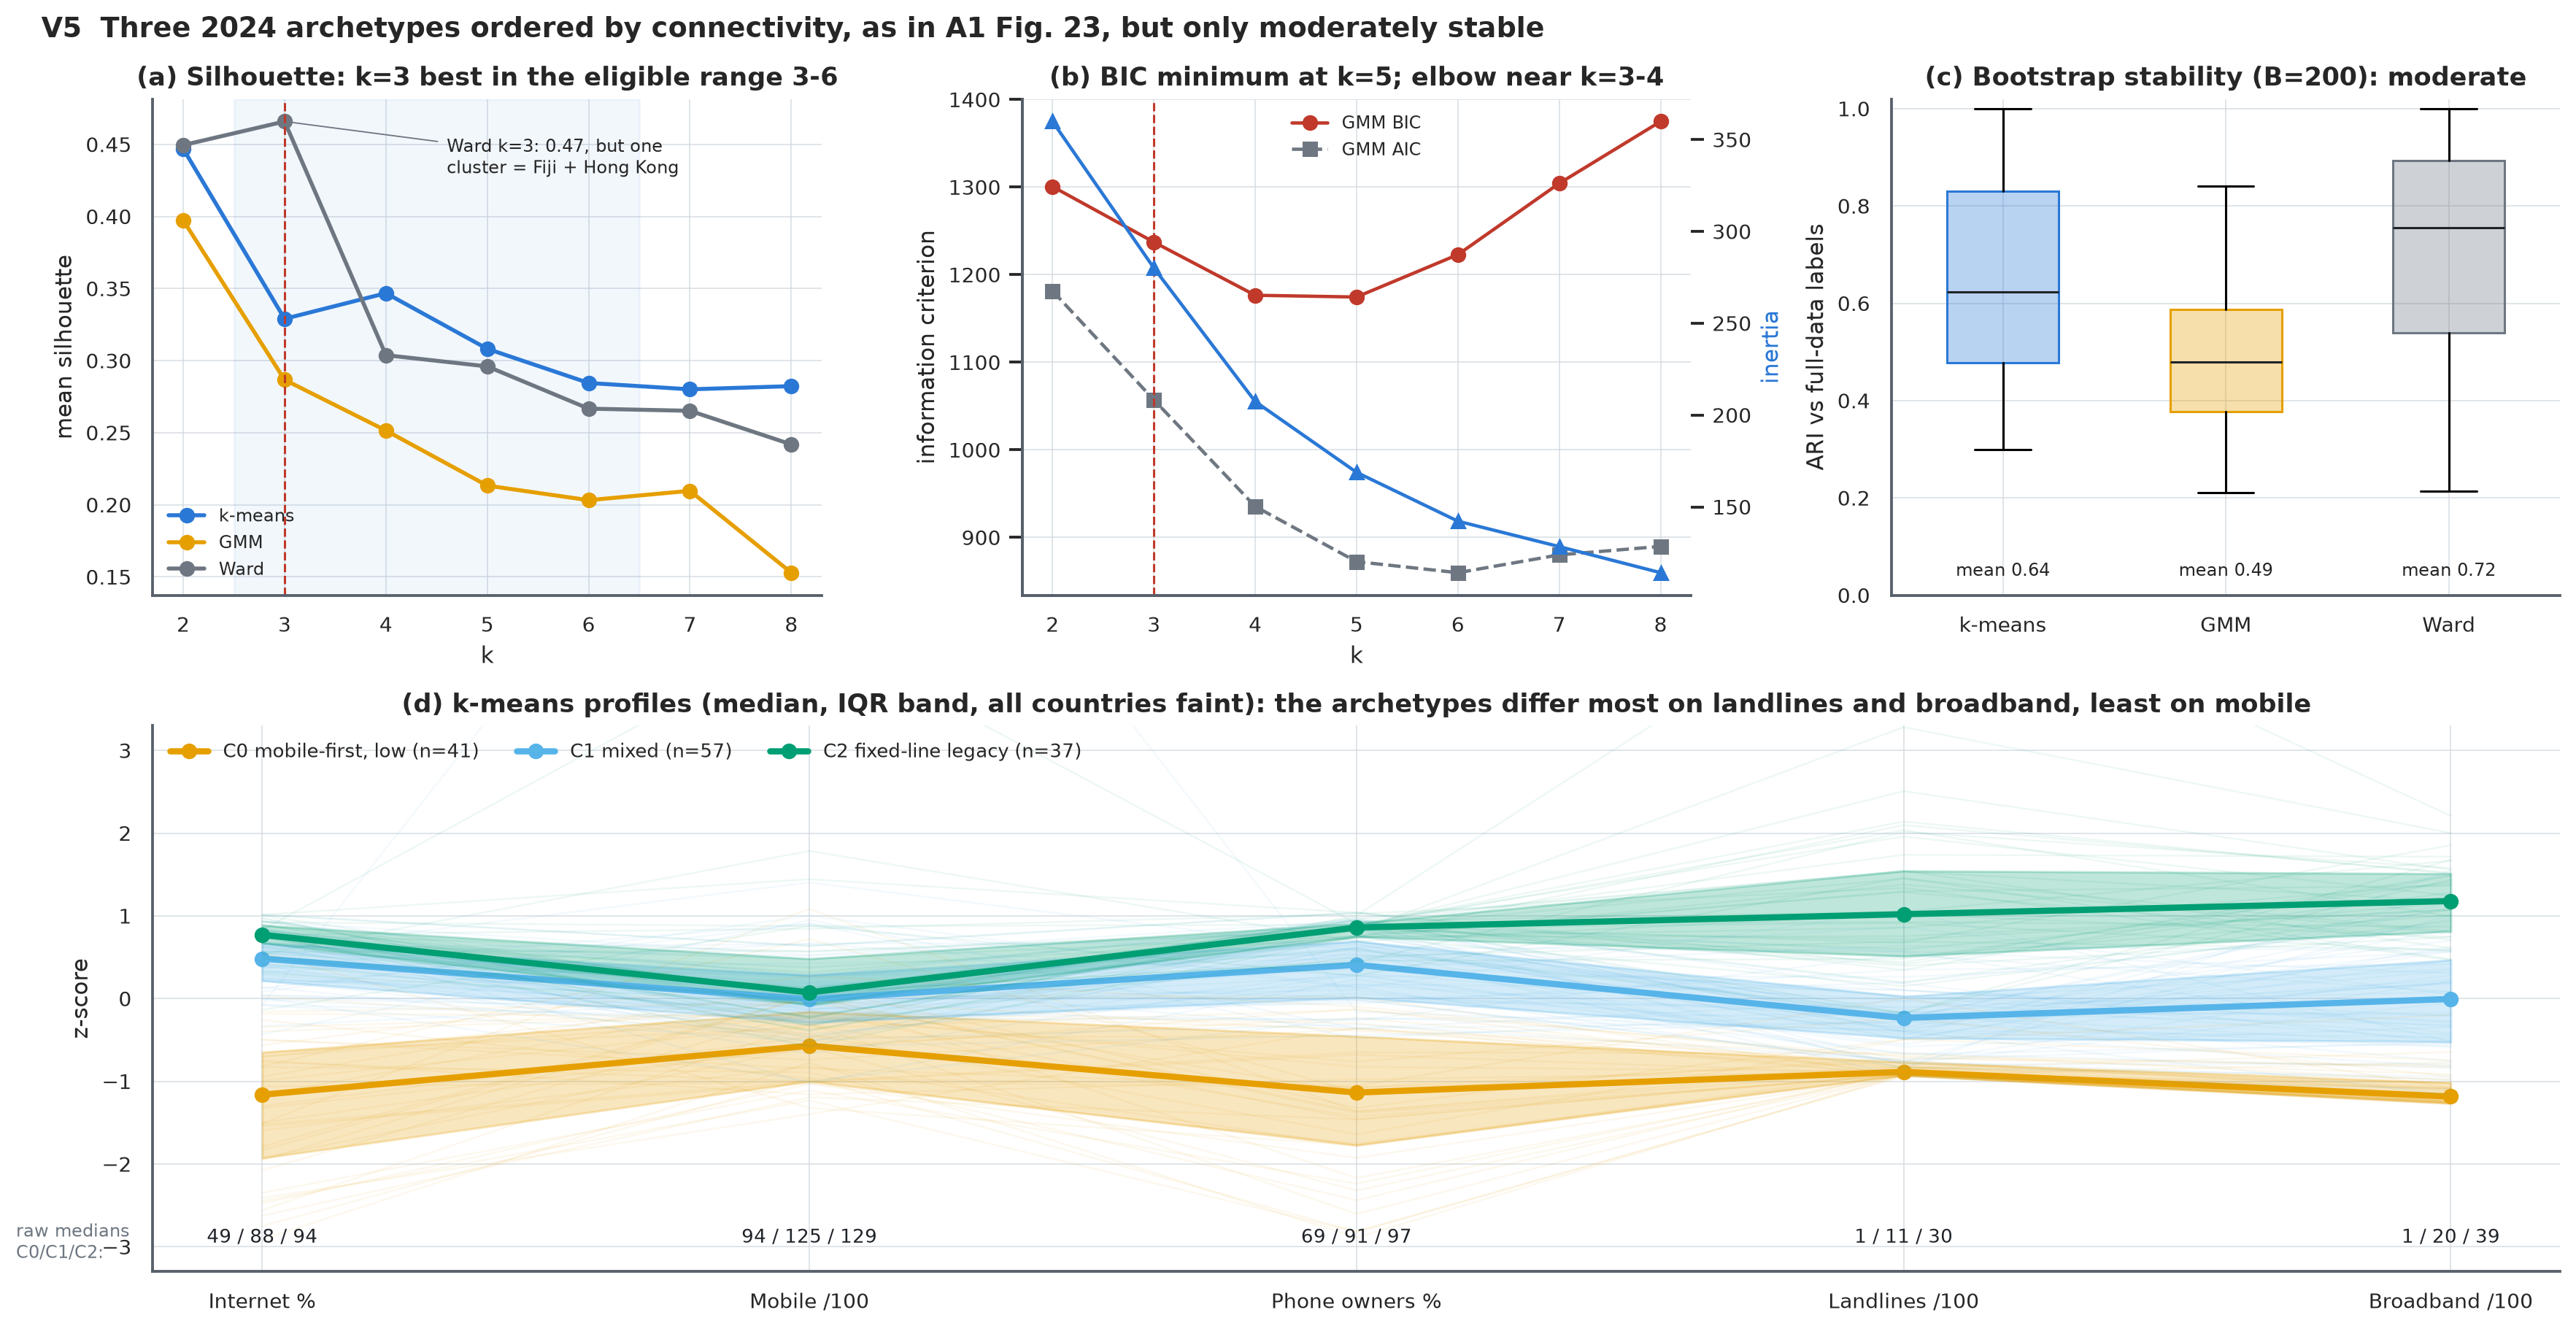
\includegraphics[width=\textwidth]{V5_cluster_validation_profiles.png}
\caption{\textbf{V5 (W2, step 2): three archetypes ordered by connectivity, separated mostly by
landlines and broadband.} (a) Silhouette against $k$ for three methods. (b) GMM BIC and AIC with
$k$-means inertia. (c) Bootstrap ARI over 200 resamples. (d) Cluster profiles as medians with IQR
bands; raw medians are printed under each axis.}
\label{fig:v5}
\end{figure*}

\textit{Stability (Fig.~\ref{fig:v5b}).} Bootstrap refits agree with the reference
labels at a mean ARI of $0.64\pm0.20$, and the co-assignment matrix shows where the disagreement lies:
mobile-first countries stay together in 92\% of refits and are almost never grouped with the legacy
group, but mixed and legacy countries share a cluster in 46\% of refits, and 45\% of all country pairs
fall between 0.1 and 0.9. Gabon (0.40), Fiji (0.50) and Venezuela (0.62) are the least stable members.
Per-country silhouettes confirm it: $k=2$ has a higher mean (0.45) but two misassigned
countries (El Salvador, South Africa), whereas $k=3$ has none, yet 15 of 135 countries, among them
Sweden, Norway, Denmark, Ireland, China and Fiji, have silhouettes below 0.10.

\begin{figure*}[!t]
\centering
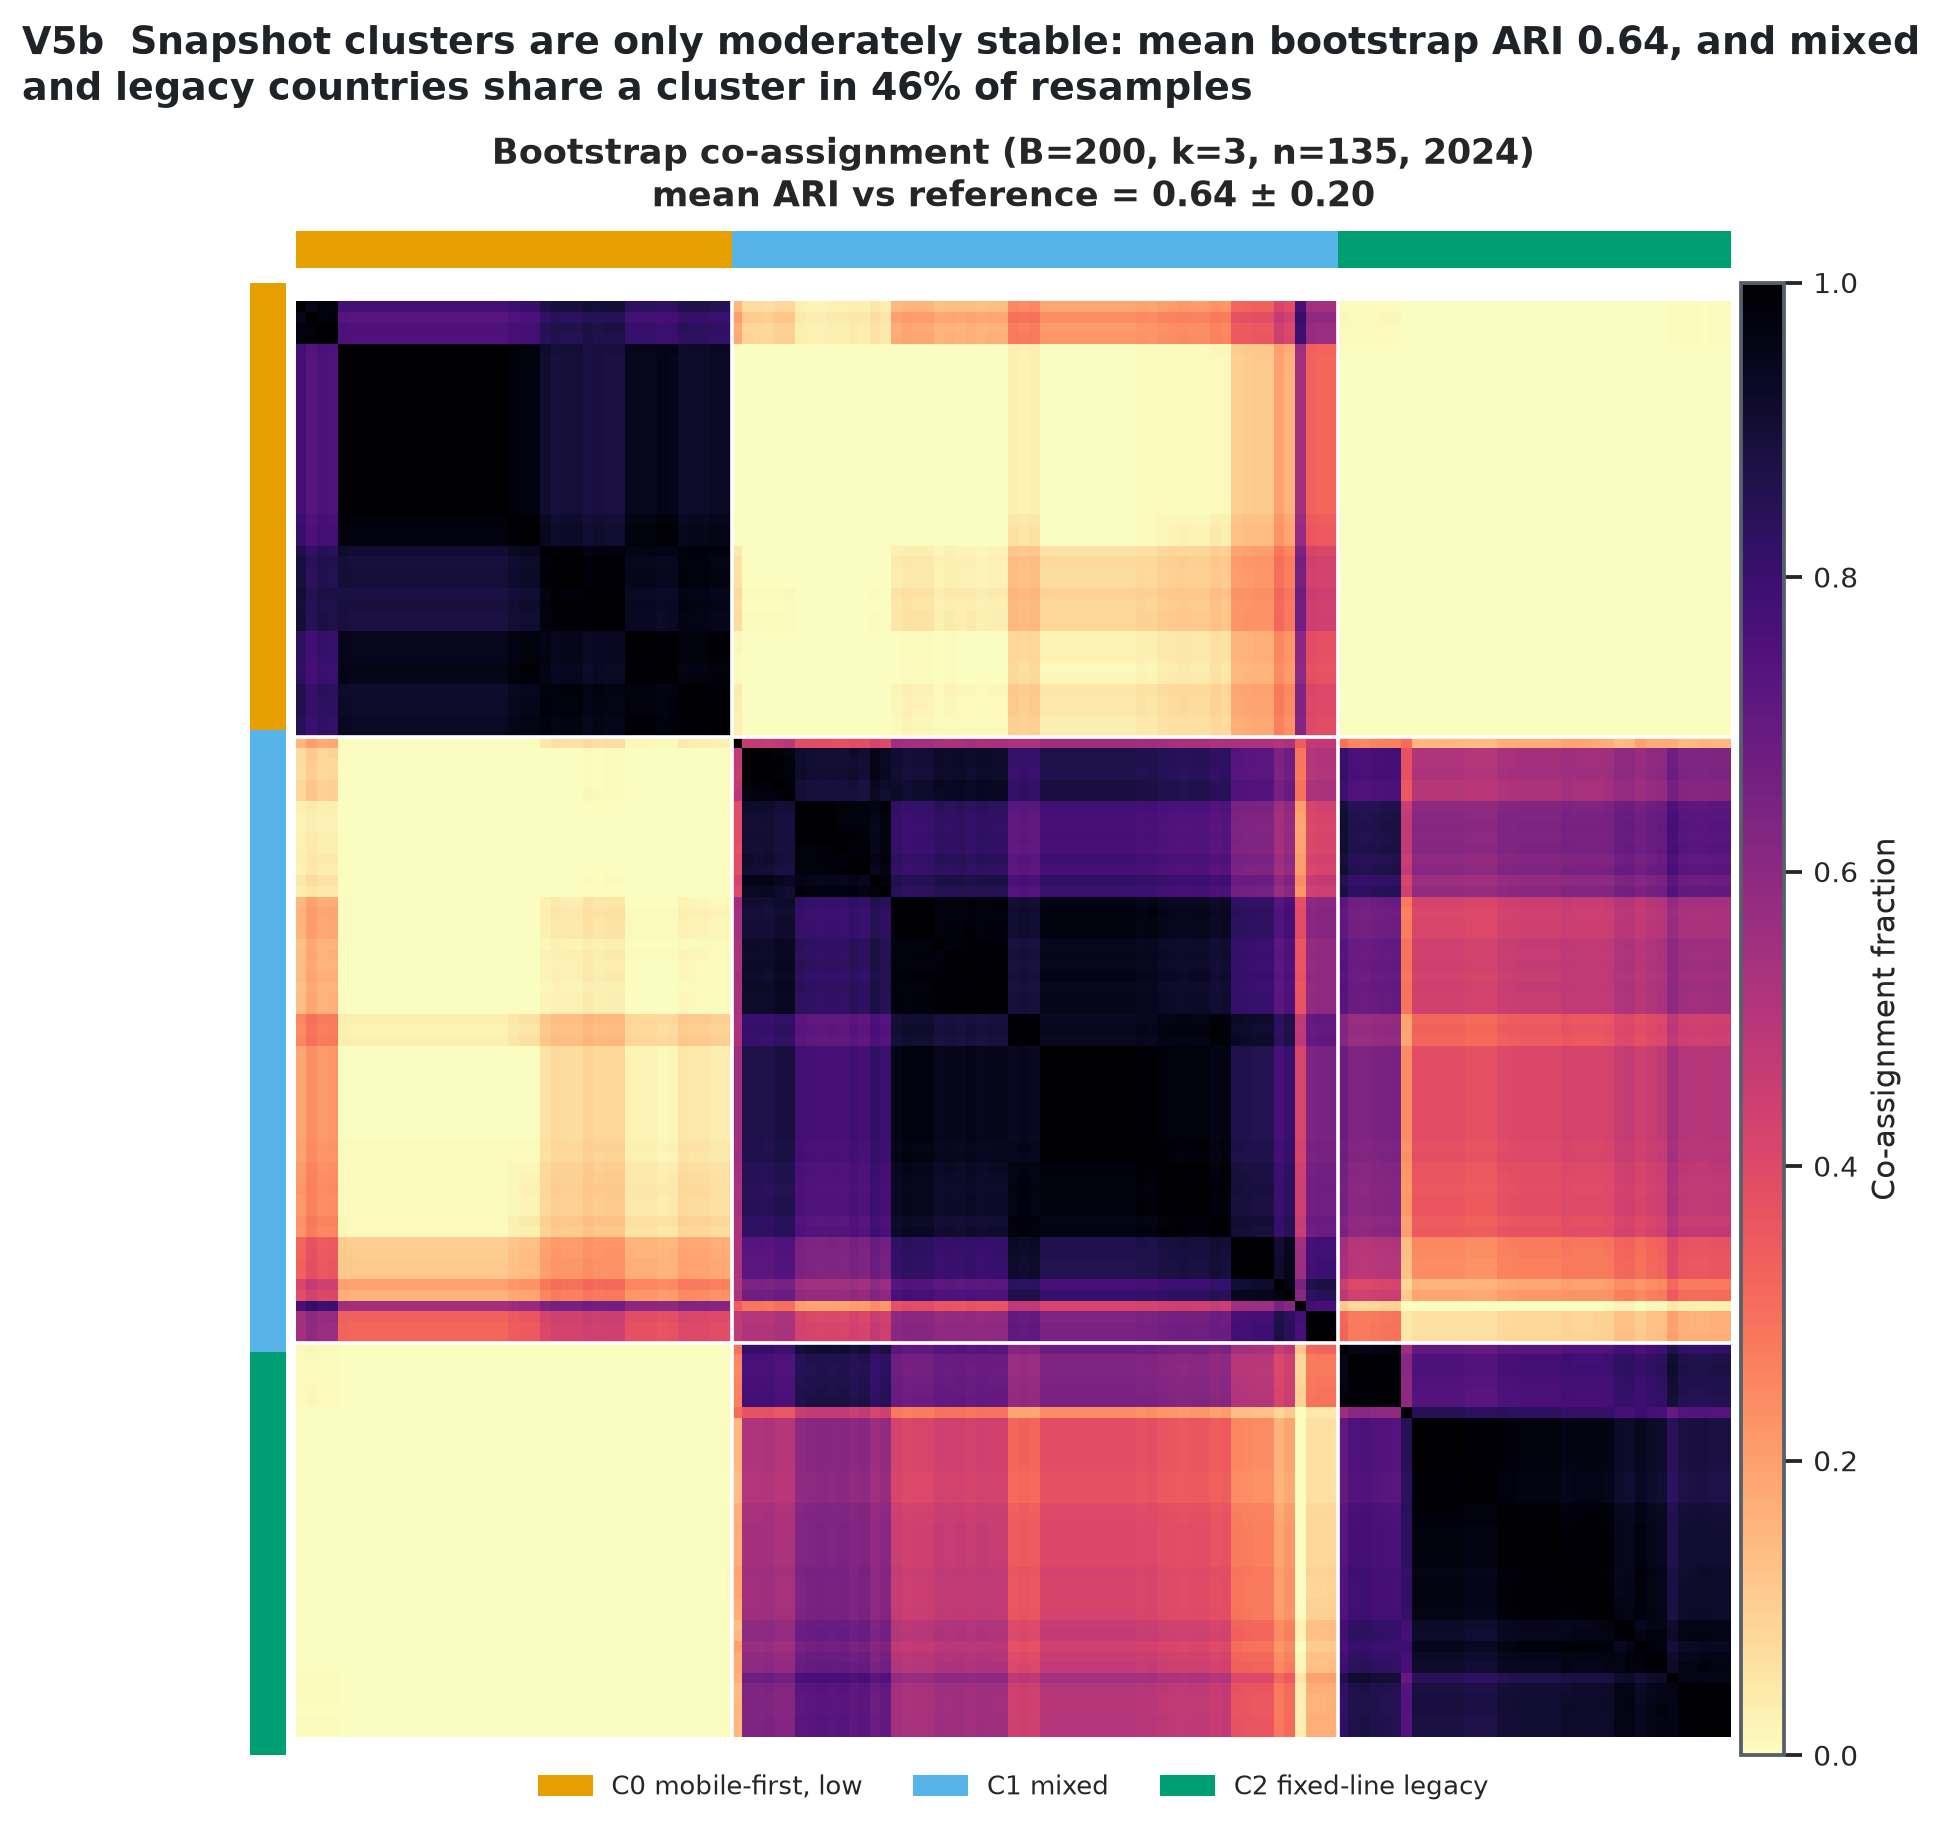
\includegraphics[width=0.78\textwidth]{V5b_bootstrap_coassignment.png}
\caption{\textbf{V5b (W2, step 3): snapshot clusters are only moderately stable.} Fraction of 200
bootstrap refits in which two countries share a cluster, ordered by cluster and by similarity within
it. Dark blocks are stable groups; the mixed--legacy off-diagonal block (about 0.46) shows where the
boundary moves.}
\label{fig:v5b}
\end{figure*}

\inference{H2.1 is refined: three types exist and are ordered by connectivity, but the boundary between
mixed and legacy countries is not stable, and a single year places many countries on it.}

\textit{Anomalies, once and over time (Figs.~\ref{fig:v6}--\ref{fig:v6c}).} Isolation Forest and LOF,
combined by rank average, share seven of their top-15 countries (Spearman 0.77), and Fiji ranks first
under both. A one-year ranking cannot say whether an outlier is a country or an error, so the
Isolation Forest was refitted in each year from 2019 to 2024 (the years with at least 100 complete
cases; 186 countries). Four countries are flagged in every year they are observed: Monaco, Hong Kong,
Andorra and Burundi; two recur (Micronesia, the United Arab Emirates); 16 are flagged only once or
twice, Fiji among them in 2023 and 2024 only; 164 are never flagged. The deviation profiles show that
each top anomaly is unusual on one indicator: Fiji (+8.1 standard deviations from its cluster mean)
and Hong Kong (+4.1) on mobile subscriptions, Monaco (+4.0) and Andorra (+2.1) on landlines, and
Uganda on low internet use and ownership ($-1.6$ each).

\begin{figure*}[!t]
\centering
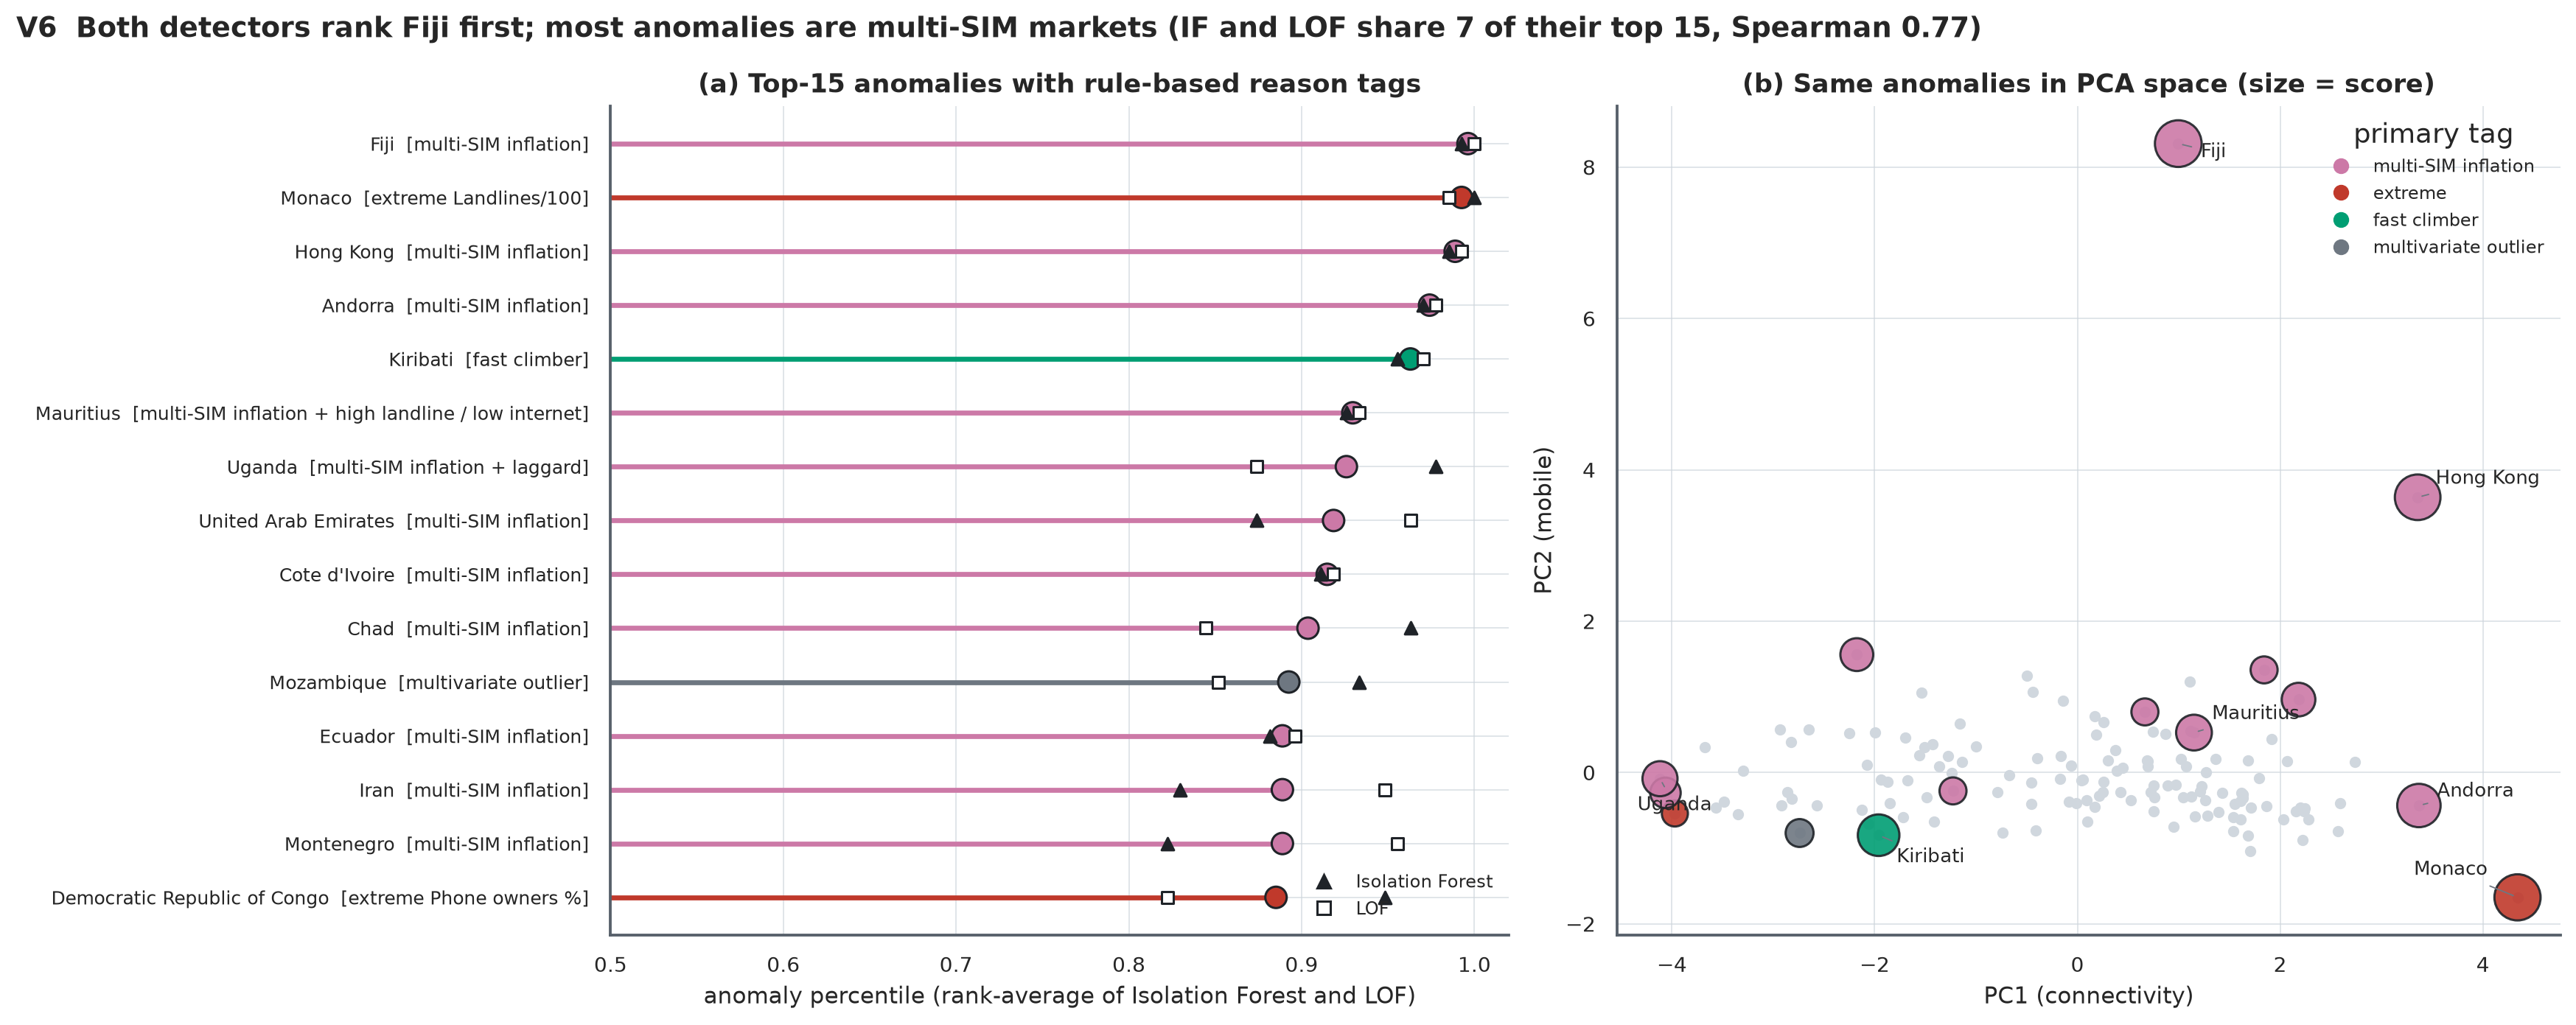
\includegraphics[width=\textwidth]{V6_anomalies.png}
\caption{\textbf{V6 (W2, step 4): both detectors rank Fiji first, and most anomalies are multi-SIM
markets.} (a) Top-15 anomaly percentiles with rule-based reason tags and each detector's percentile.
(b) The same countries in PCA space, sized by anomaly score.}
\label{fig:v6}
\end{figure*}

\begin{figure}[!t]
\centering
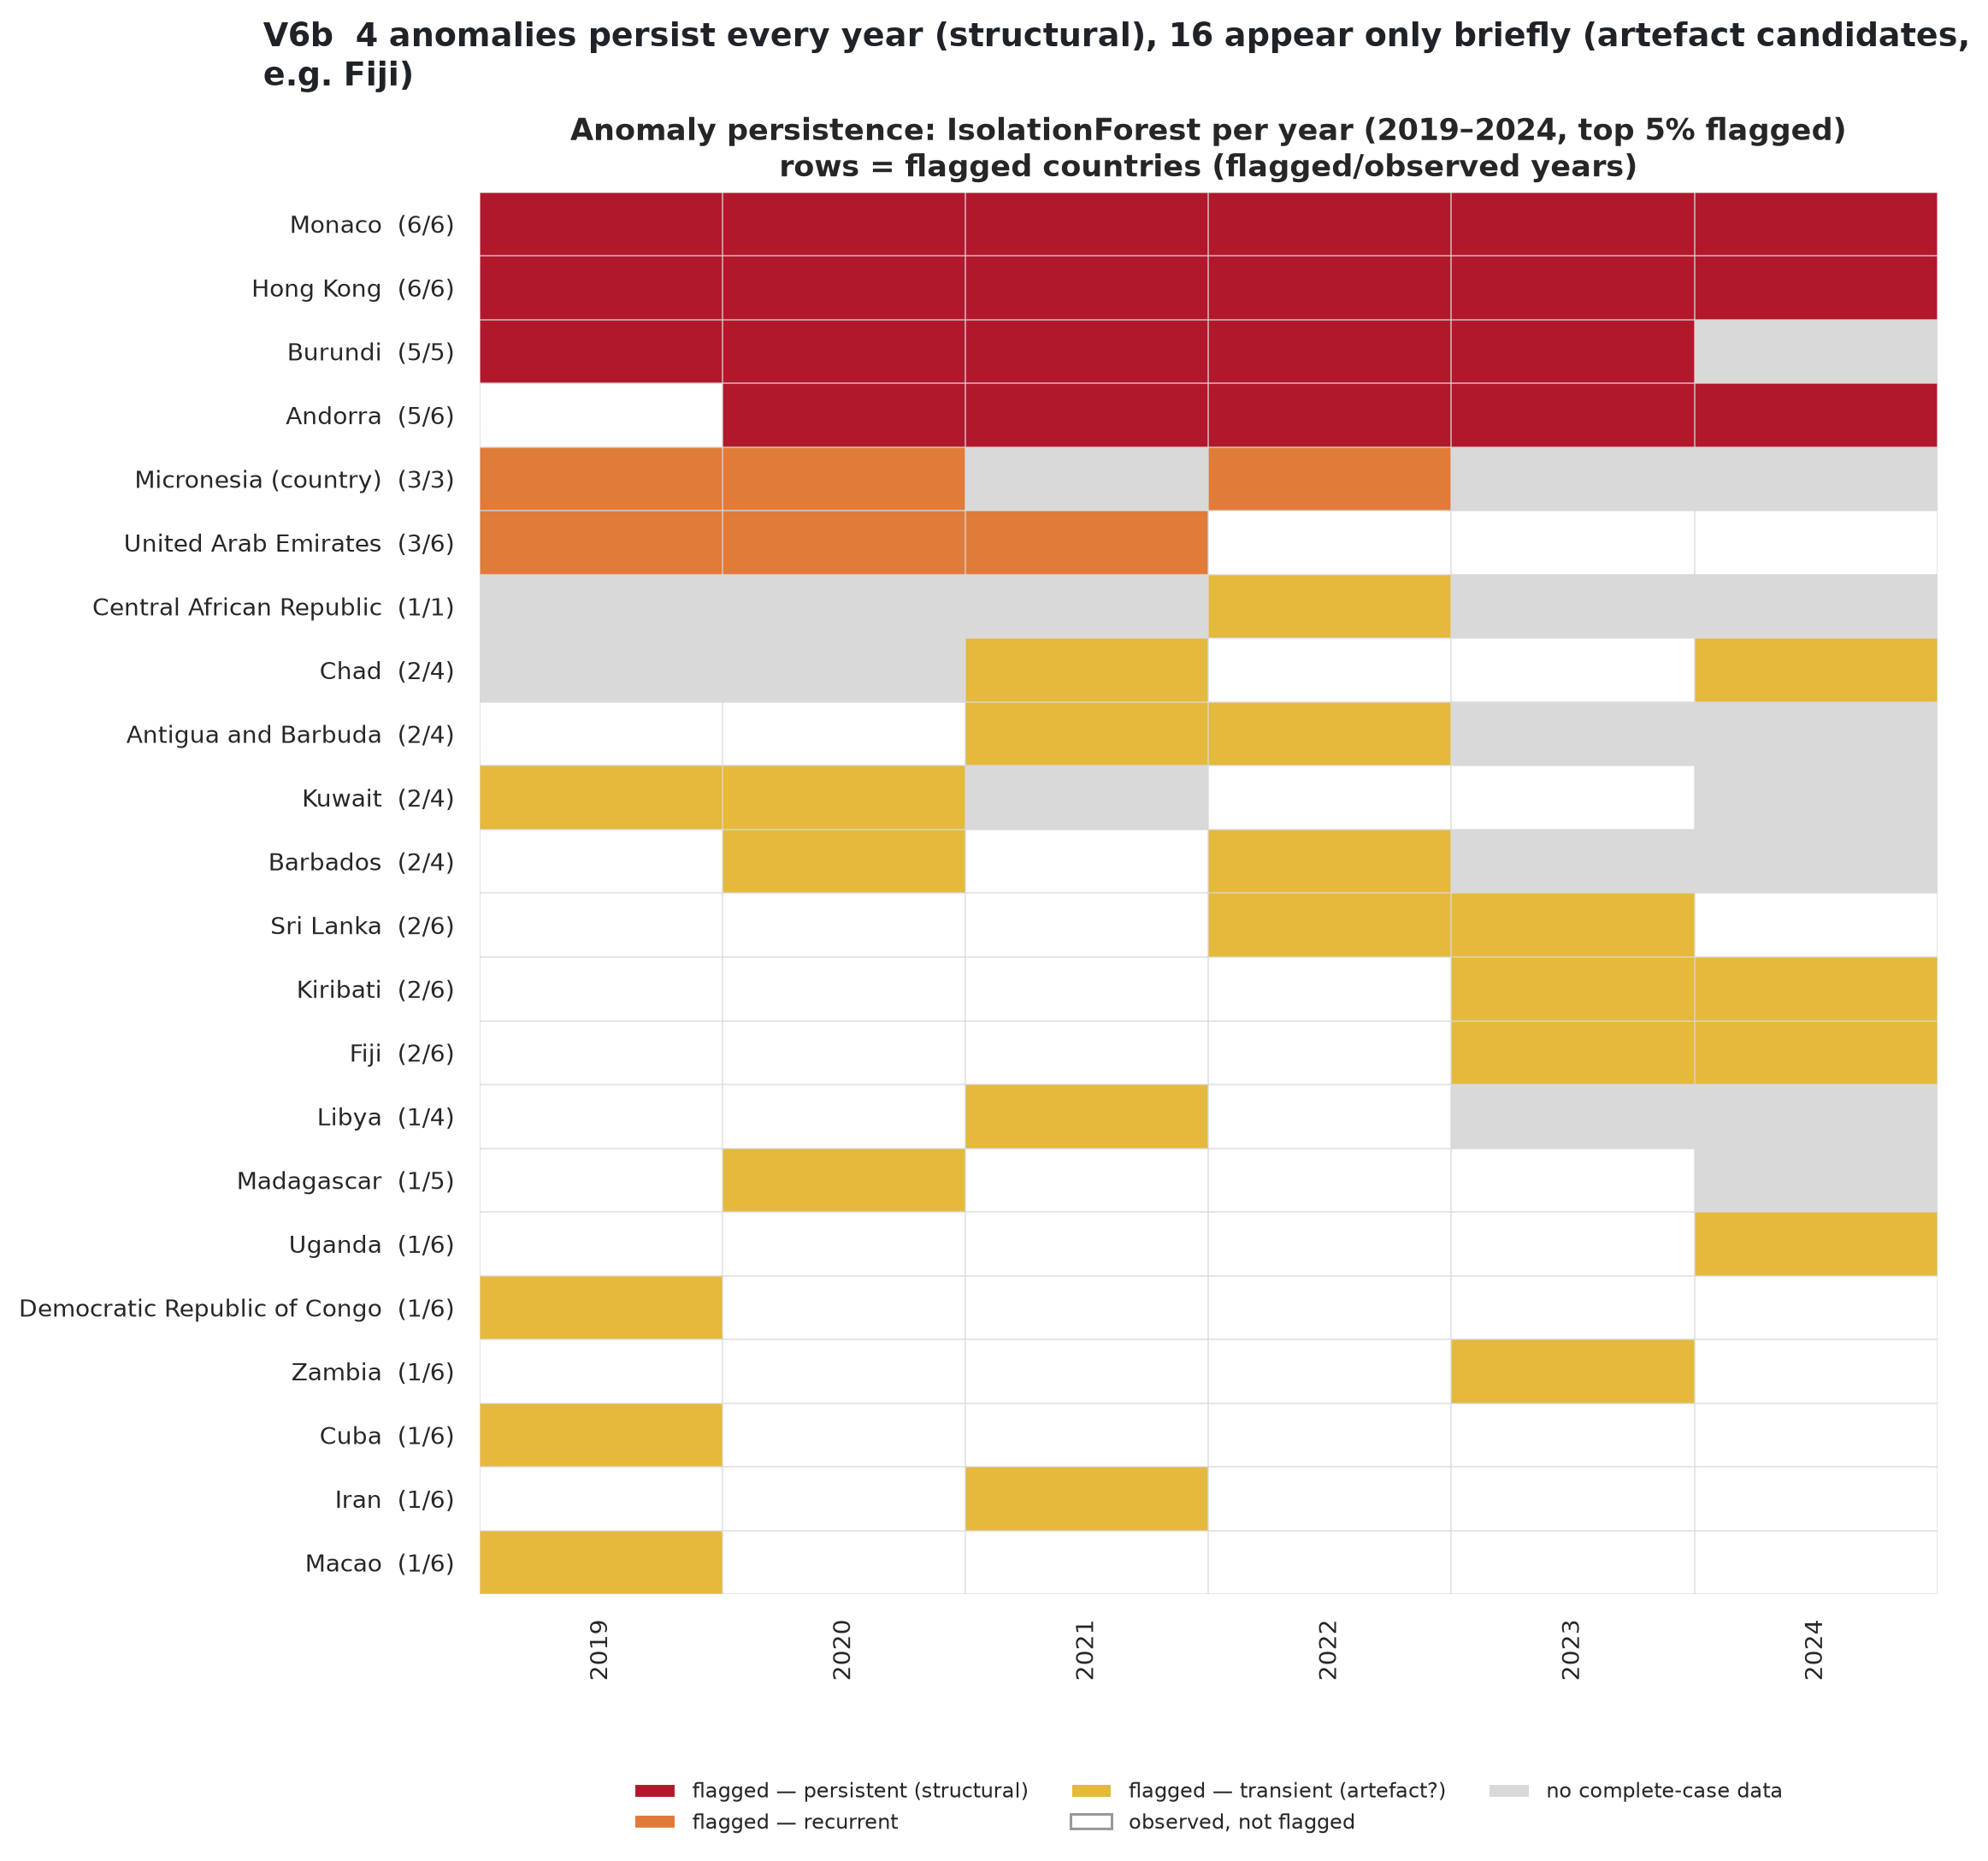
\includegraphics[width=\columnwidth]{V6b_anomaly_persistence.png}
\caption{\textbf{V6b (W2, step 4): four anomalies persist every year; Fiji appears only in 2023--24.}
Per-year Isolation Forest flags, 2019--2024; colour encodes the persistence class, grey marks years
without complete data.}
\label{fig:v6b}
\end{figure}

\begin{figure}[!t]
\centering
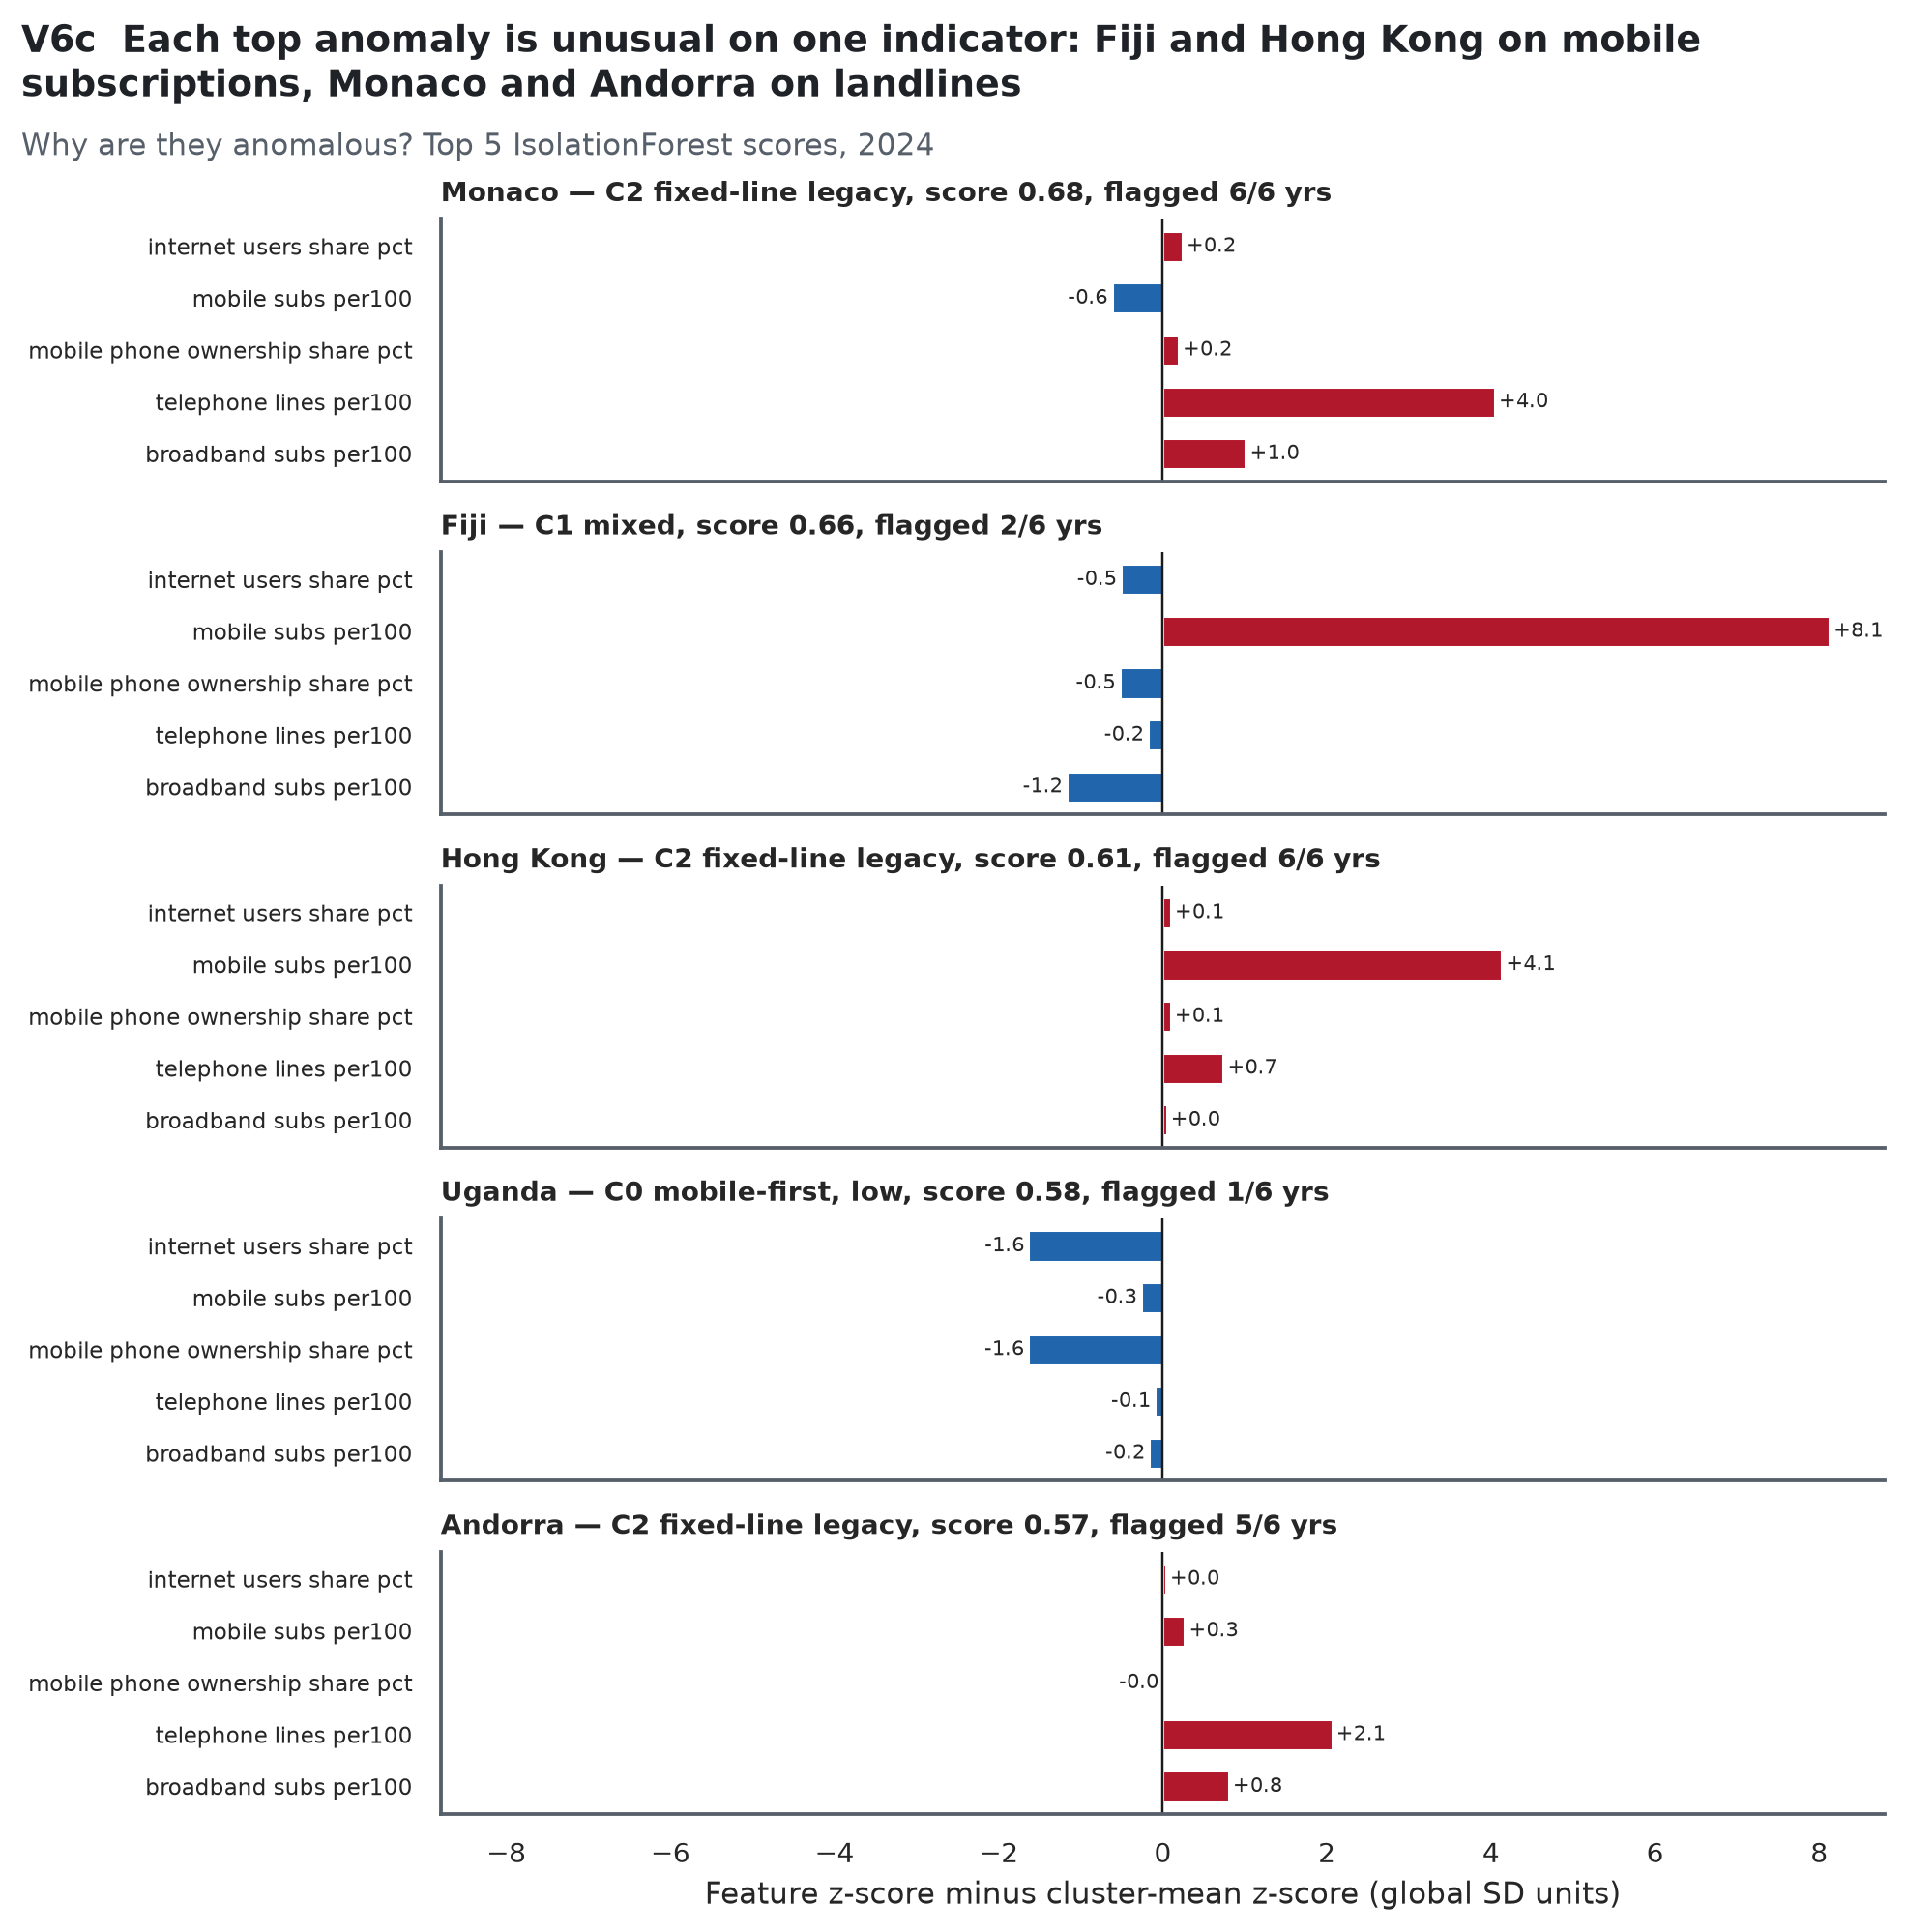
\includegraphics[width=\columnwidth]{V6c_anomaly_why.png}
\caption{\textbf{V6c (W2, step 5): each top anomaly is unusual on one indicator.} Feature z-score minus
the cluster-mean z-score for the five highest 2024 scores.}
\label{fig:v6c}
\end{figure}

\inference{H2.2 is refined: persistent anomalies are real markets (multi-SIM, legacy landlines) and are
kept, whereas a transient anomaly such as Fiji is a recording error. A snapshot cannot tell the two
apart; persistence over time can.}

\subsection{Inferences $K_1$ and the feedback loop}
Three inferences leave iteration~1 (W2 rows of Table~\ref{tab:loops}): the snapshot clusters are only
moderately stable (K1.1); Fiji is a transient anomaly and therefore an artefact, whereas Monaco and Hong
Kong are structural (K1.2); and one year cannot show a path (K1.3). The transformation is a change of
data representation and of distance. Artefacts are removed by the shared rule (T1). Each country
becomes its 2000--2025 internet curve (T2): 181 countries have at least 18 of 26 years observed, and 225
interior cells are interpolated. Curves are compared by dynamic time warping (T3), which aligns them
under a band of five years, and grouped by average linkage (T4). Fig.~\ref{fig:v8a} justifies T3: Brazil
and Bolivia cross 50\% in 2012.6 and 2019.2, 6.6 years apart, along almost the same curve; DTW scores
them 0.17 apart, five times closer than the same-year distance of 0.86.

\begin{figure*}[!t]
\centering
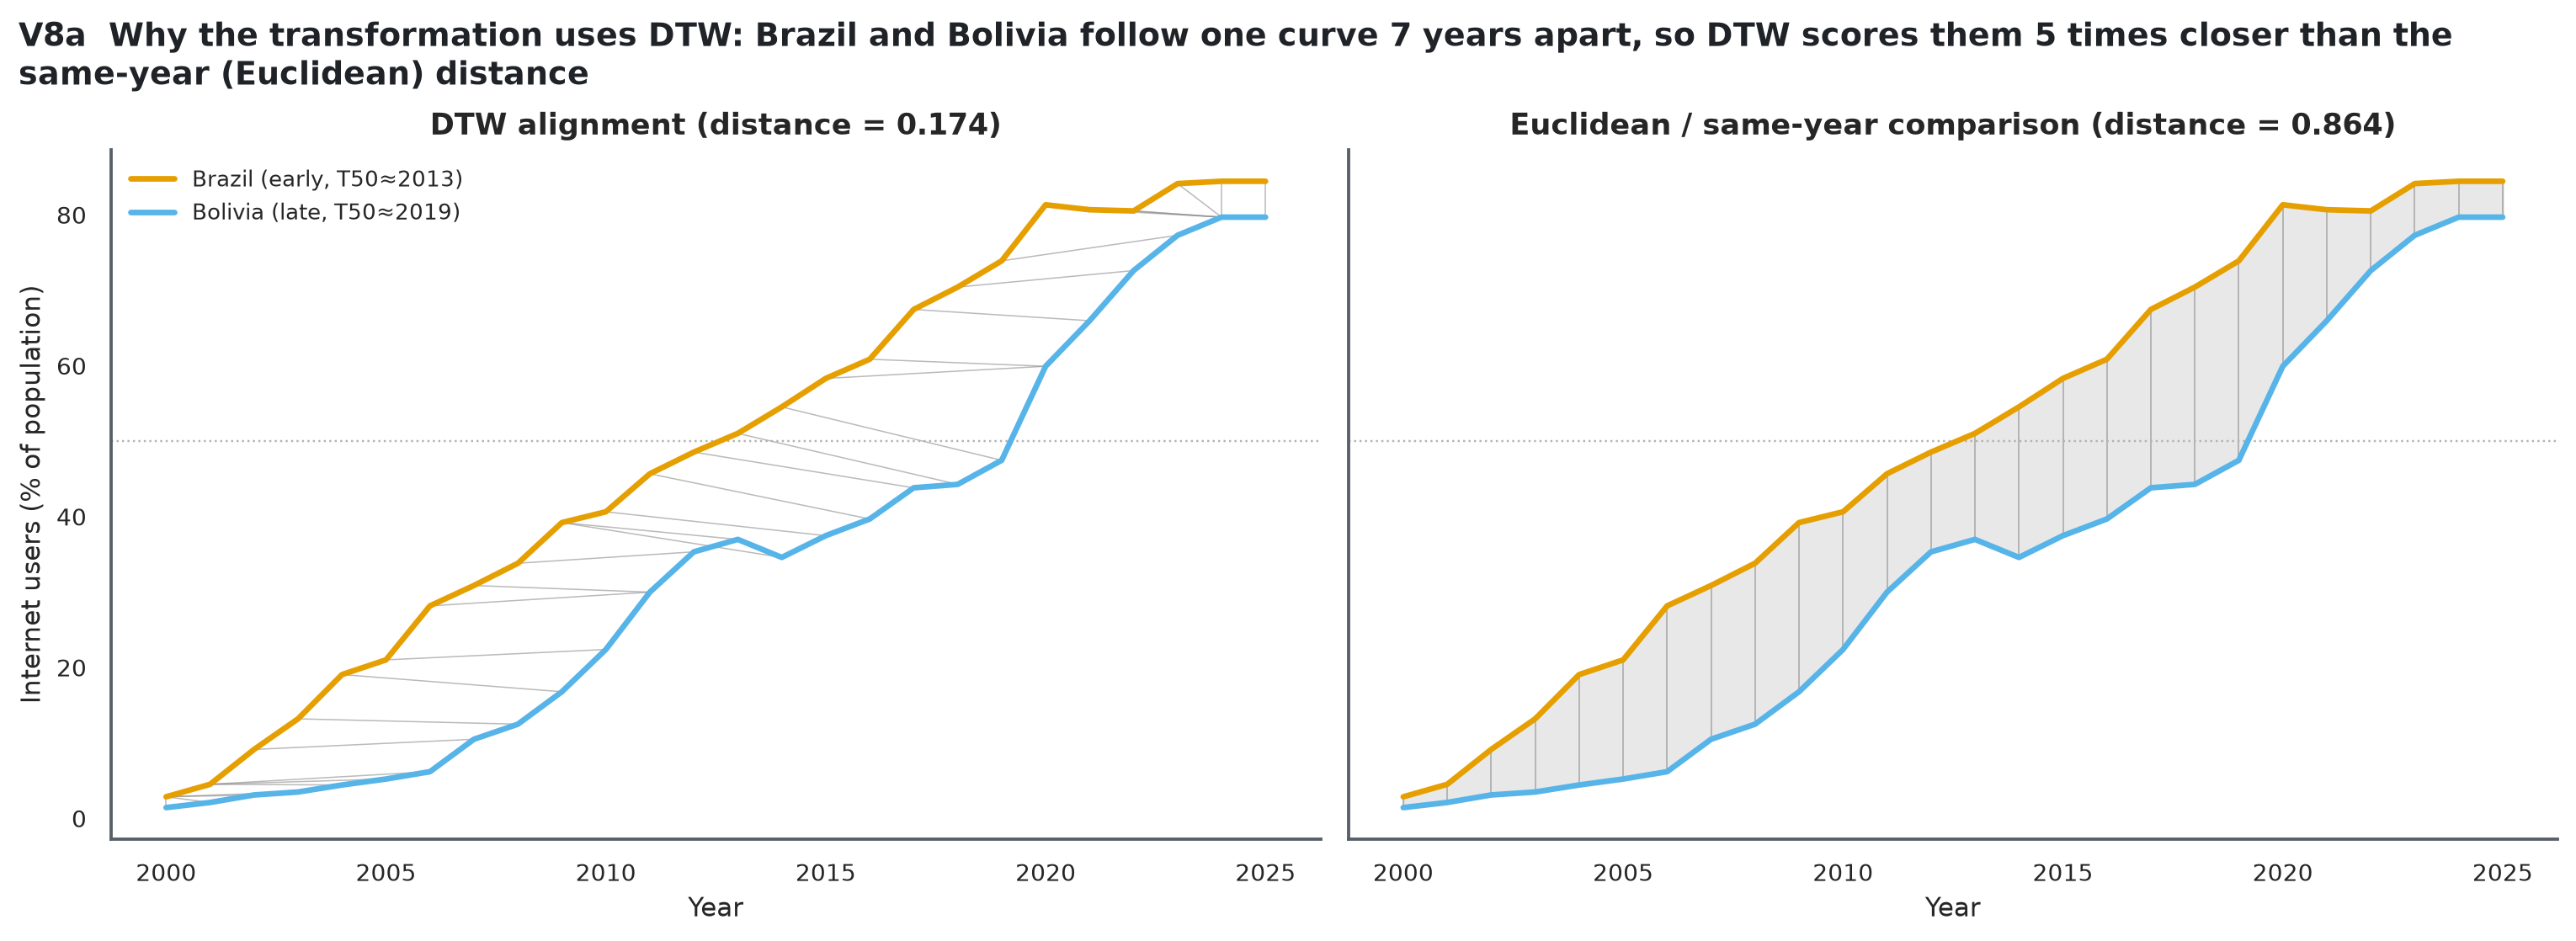
\includegraphics[width=\textwidth]{V8a_dtw_alignment.png}
\caption{\textbf{V8a (W2, step 6): why the transformation uses DTW.} The same pair of curves compared
along DTW's warping path (left, grey connectors) and year by year (right, shaded gap).}
\label{fig:v8a}
\end{figure*}

\subsection{Iteration 2: trajectories under DTW}
\textit{The hierarchy.} The DTW dendrogram preserves distances well (cophenetic
correlation 0.72). Its first split separates 43 late starters from all other countries; the second
separates 25 early saturators from a majority of 113 (silhouette 0.54 at $k=3$). The next cut only
splits off a single country, so $k=3$ is the natural cut. Leaf colours show that geography explains
part, not all, of the tree: 33 of 51 African countries are late starters, every South American country
is in the majority, and 16 of 42 European countries are early saturators.

\textit{The archetypes (Fig.~\ref{fig:v8}).} T0 late starters (43 countries, medoid Tanzania, median
0\%$\rightarrow$33\%), T1 the S-curve majority (113, Maldives, 3\%$\rightarrow$84\%) and T2 early
saturators (25, South Korea, 39\%$\rightarrow$96\%). The trajectory labels are far better separated in
trajectory space than the snapshot labels (silhouette 0.52 against 0.35 on the 133 shared countries).

\begin{figure*}[!t]
\centering
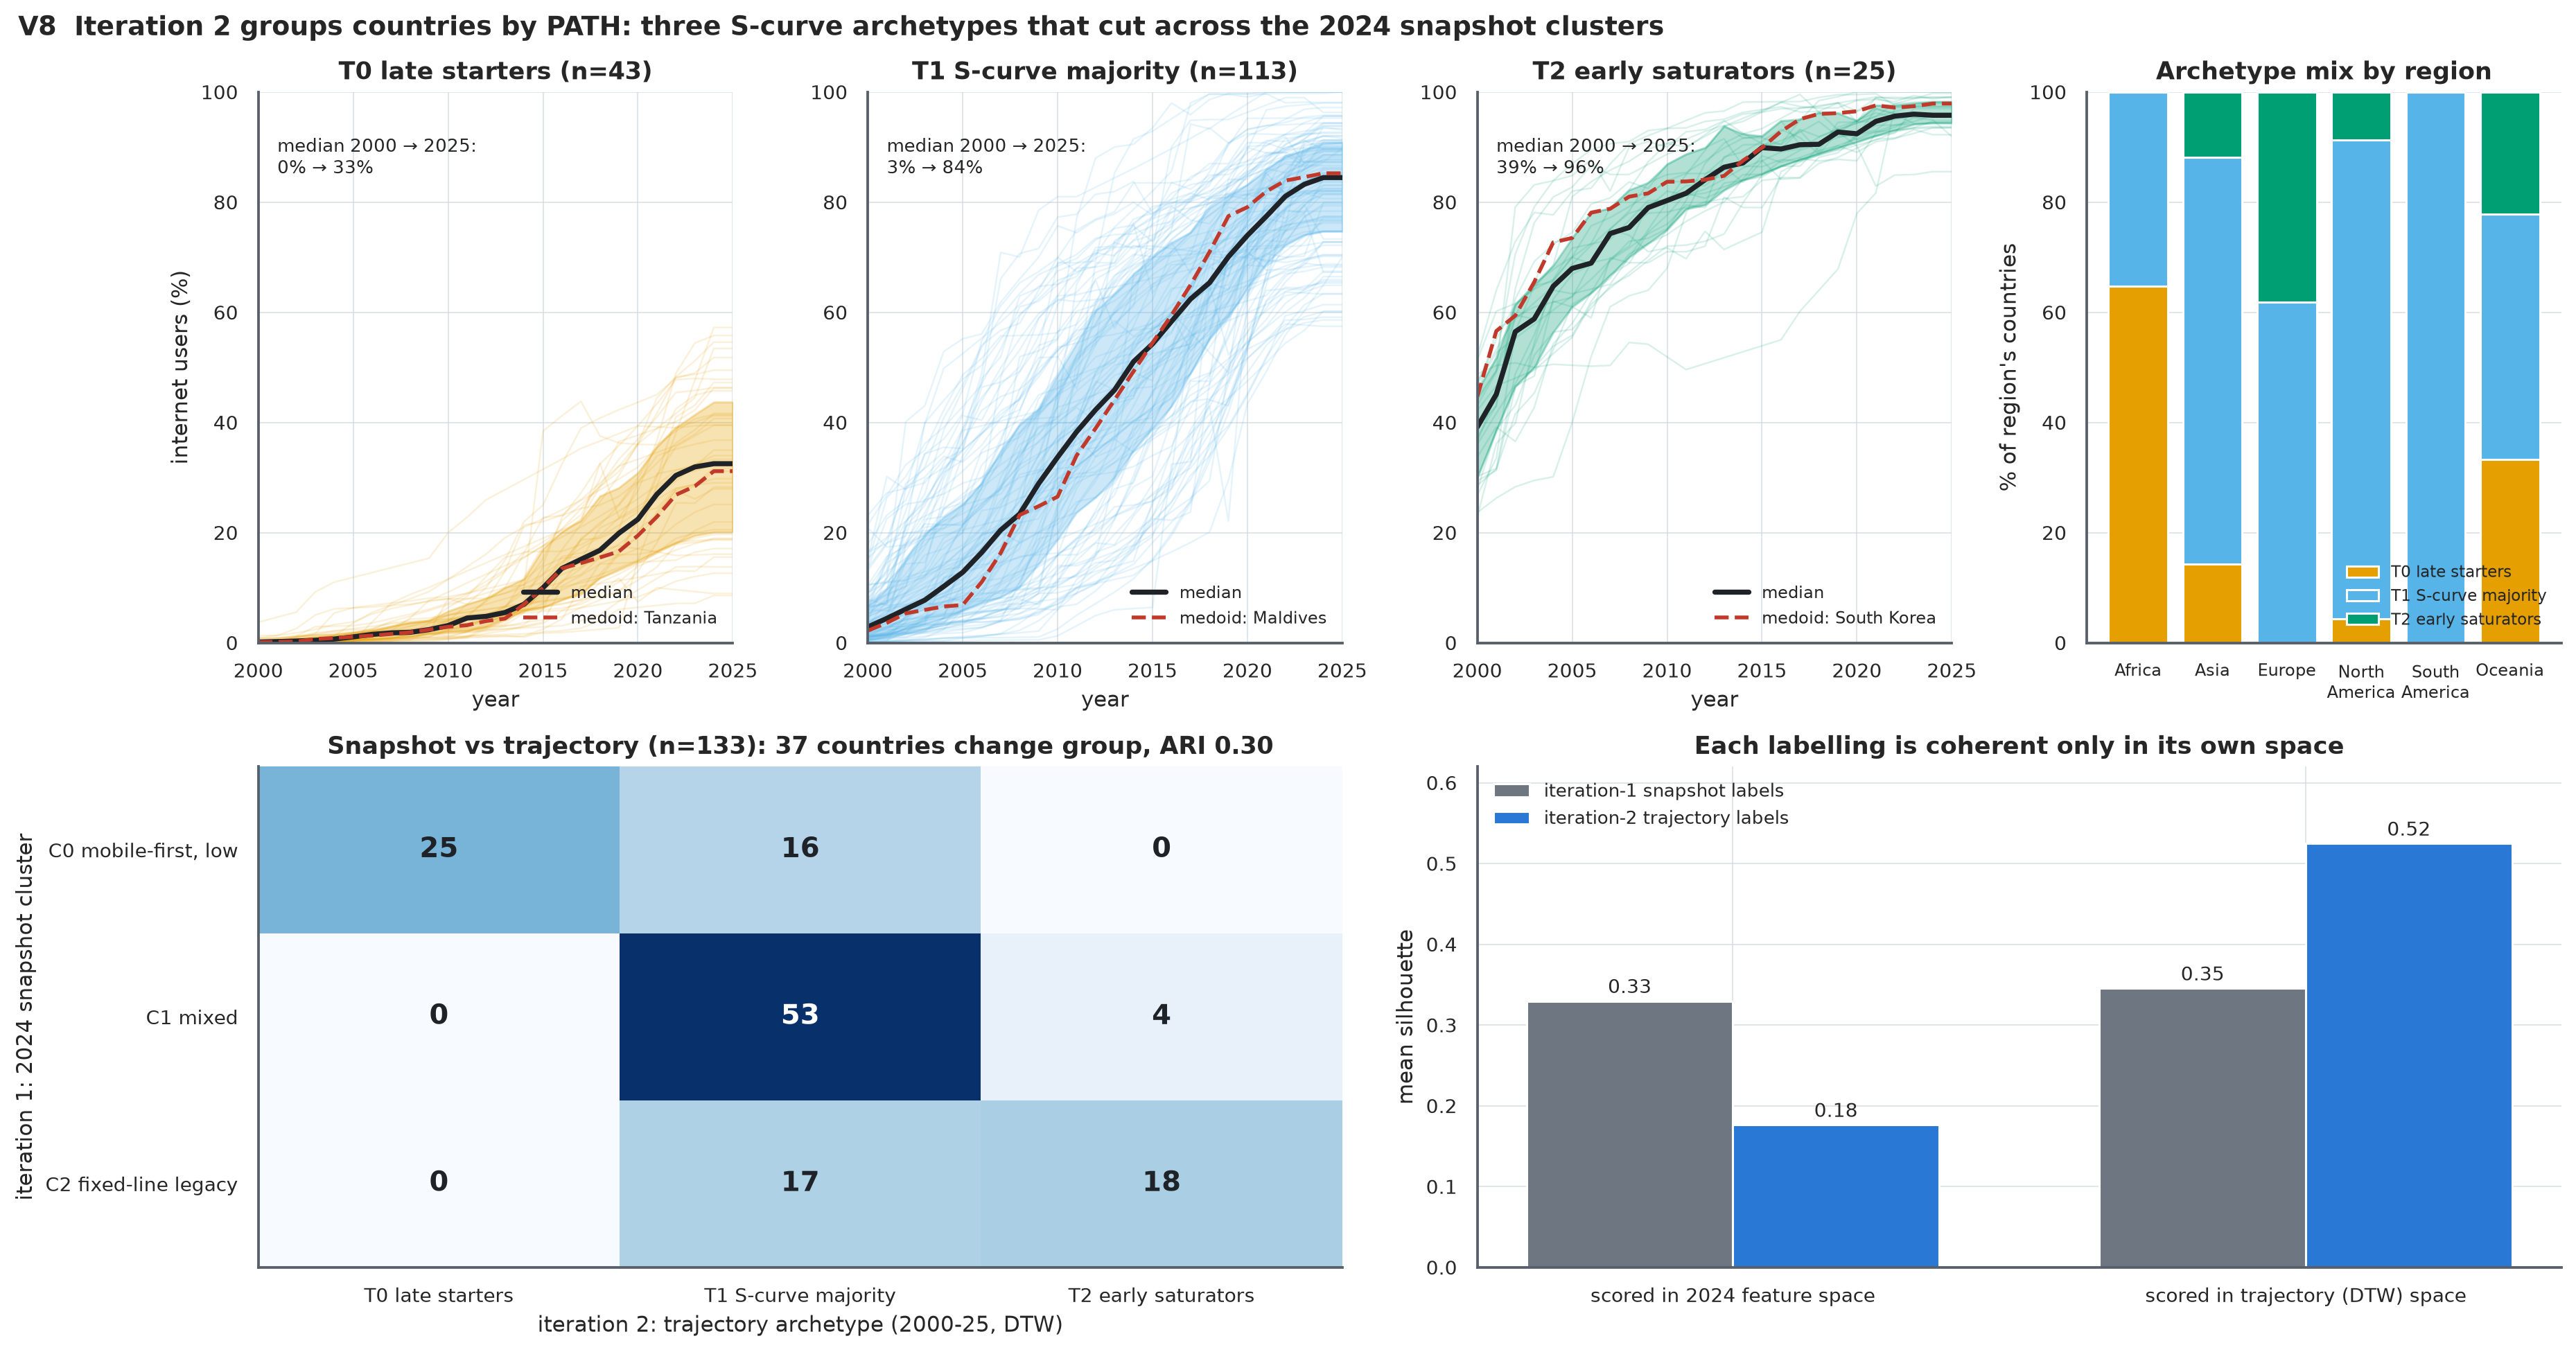
\includegraphics[width=\textwidth]{V8_trajectory_archetypes.png}
\caption{\textbf{V8 (W2, step 7): grouping by path yields three S-curve archetypes that cut across the
2024 snapshot clusters.} Top: the three DTW archetypes (all members faint, IQR band, median, medoid) and
their mix by region. Bottom left: snapshot clusters against trajectory archetypes ($n=133$). Bottom
right: each labelling is coherent only in its own space.}
\label{fig:v8}
\end{figure*}

\textit{Timing.} The archetypes are ordered in time: the median year of crossing
50\% is 2001 for early saturators, 2014 for the majority and 2023 for the five late starters that have
crossed (38 have not). The majority, however, spans 17 years, and a Euclidean $k$-means on the same
curves aligns more closely with timing ($\eta^2=0.82$ against 0.59 for DTW). This is the intended
behaviour of T3: DTW groups curves by shape and tolerates shifts, so the majority is one shape reached
at different times, which is W1's delay finding seen from the clustering side.

\textit{What the feedback loop changed (Fig.~\ref{fig:v8d}).} On the 133 countries present in both
iterations, the two labellings agree only weakly (ARI 0.30) and 37 countries change group after
Hungarian matching. Sixteen low-connectivity countries of 2024, including India, Indonesia and Ghana,
lie on the majority curve, only later; 17 fixed-line-legacy countries, including Italy, Spain and
Portugal, reached their level along the majority curve rather than by early saturation; and four mixed
countries (Sweden, Norway, Finland, New Zealand) are early saturators. Movers had weaker iteration-1
membership (median silhouette 0.28 against 0.39 for countries that stayed).

\begin{figure*}[!t]
\centering
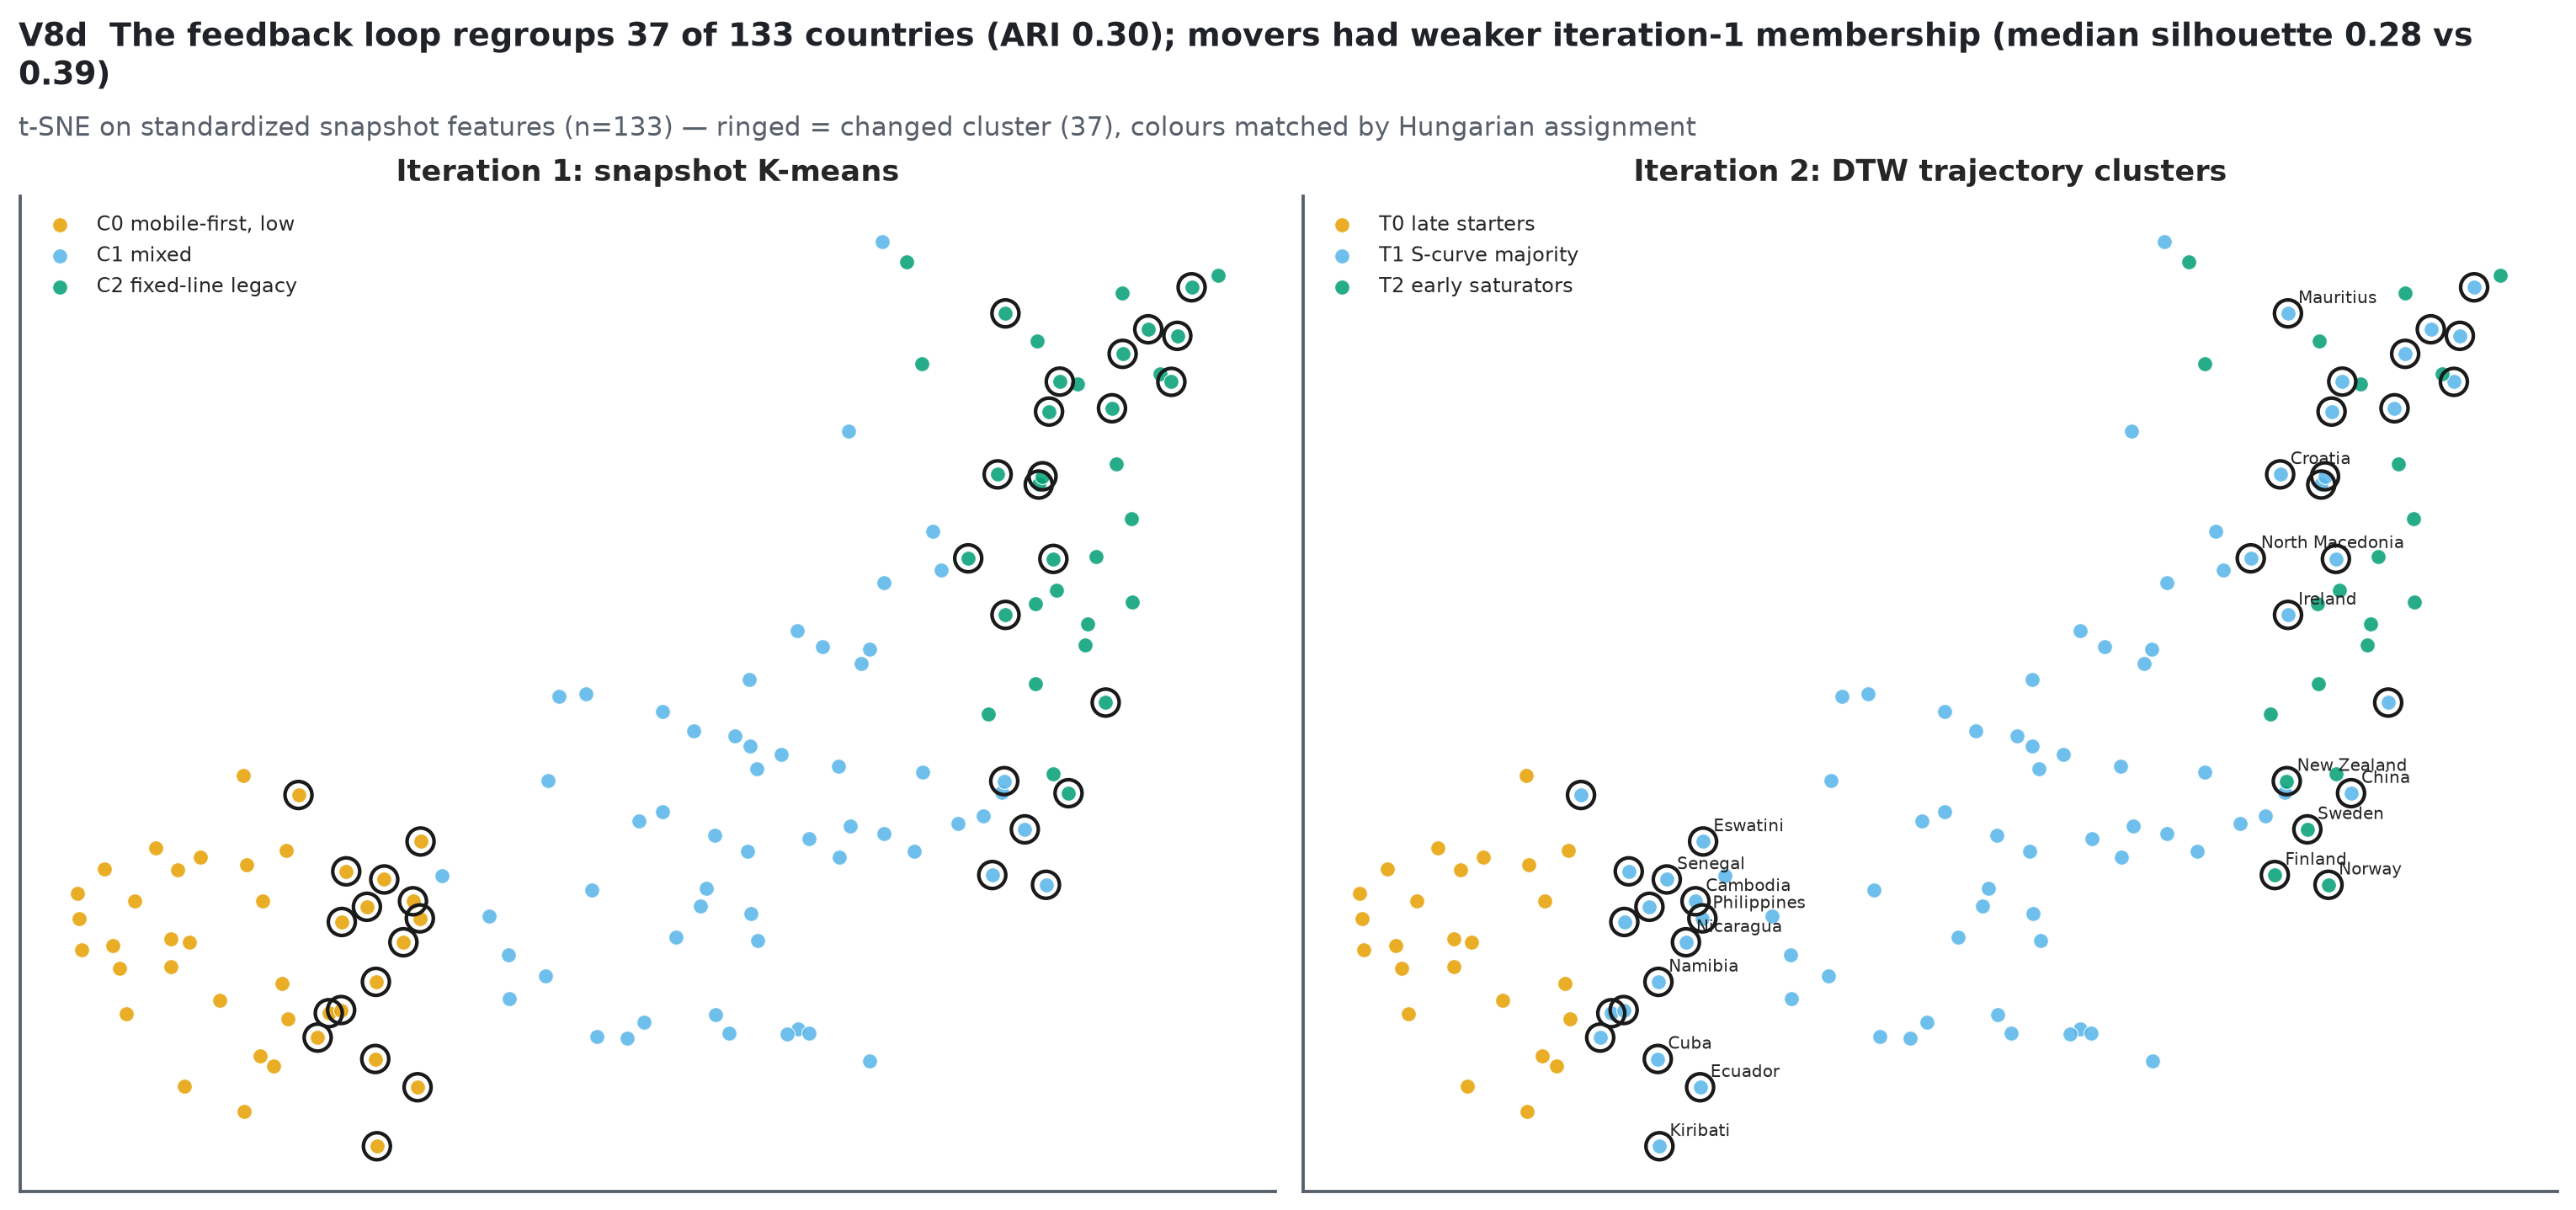
\includegraphics[width=\textwidth]{V8d_iteration_embedding.png}
\caption{\textbf{V8d (W2, step 8): the feedback loop regroups 37 of 133 countries.} The same t-SNE
map~\cite{vandermaaten2008} of the snapshot features coloured by iteration-1 clusters (left) and
iteration-2 archetypes (right); colours matched by the Hungarian method, movers ringed.}
\label{fig:v8d}
\end{figure*}

\subsection{Knowledge $K_2$ and the analysis path}
H2.3 is rejected: countries at the same level today followed different paths, and grouping by path
moves more than a quarter of them. H2.4 is refined: the archetypes are ordered in time, but within the
majority timing varies by 17 years along one shape. Country archetypes are therefore paths rather than
positions, and iteration~2 recovers A1's ``same place today, opposite histories'' with a model instead
of a visual comparison.

\textit{Analysis path.} The biplot (V4) showed structure and two extreme countries; the $k$ scan (V5)
chose three groups; because a single ARI hides where groups are unstable, co-assignment (V5b) and
per-country silhouettes located the unstable boundary. The anomaly ranking (V6) raised the question of error
versus behaviour, which persistence (V6b) and deviation profiles (V6c) answered. After $T$, V8a
justified the distance, the dendrogram fixed $k=3$, V8 described the archetypes, timing was checked and V8d
measured what the loop changed. The result enters the synthesis (V14c).

% =========================================================================================
\section{Workflow W3: Supervised Learning}\label{sec:w3}
% =========================================================================================
\begin{figure*}[p]
\centering
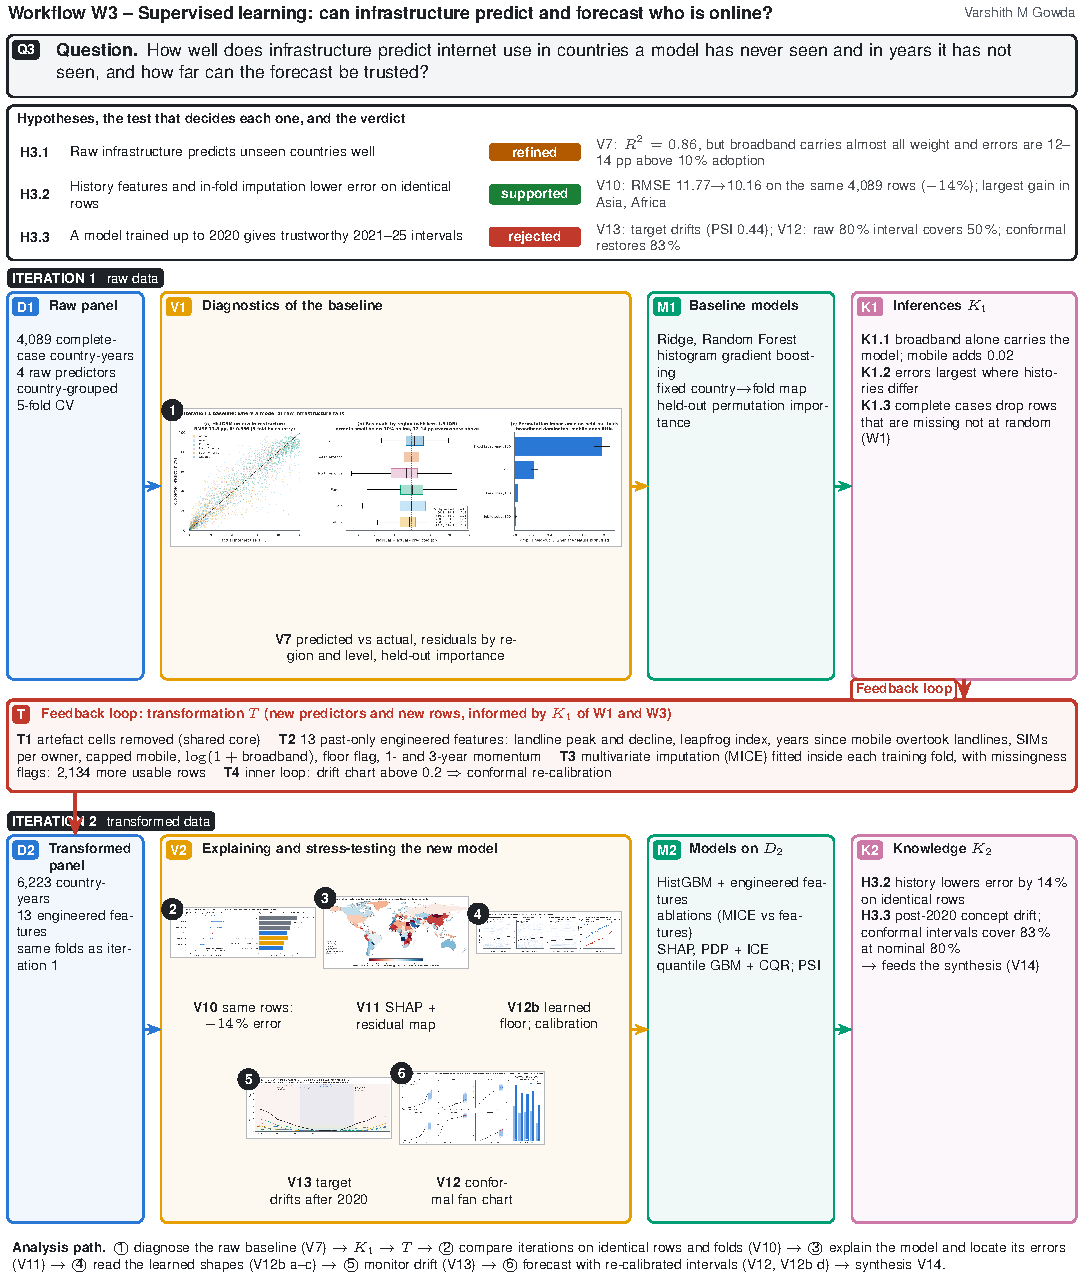
\includegraphics[width=\textwidth,height=0.92\textheight,keepaspectratio]{W3_workflow_supervised.pdf}
\caption{\textbf{Workflow W3, supervised learning, unrolled.} Question and hypotheses (top); iteration~1
with the baseline diagnostics; the feedback loop $T$, which adds history features defined by W1's
inferences and imputed rows, and an inner drift-triggered re-calibration; iteration~2 with five
figures; the numbered analysis path (bottom).}
\label{fig:w3}
\end{figure*}

\hyp{Q3.}{How well does infrastructure predict internet use in countries a model has never seen and in
years it has not seen, and how far can the forecast be trusted?}
Three hypotheses are tested (Fig.~\ref{fig:w3}): H3.1 raw infrastructure predicts unseen countries
well; H3.2 history features and in-fold imputation lower error on identical rows; H3.3 a model
trained up to 2020 gives trustworthy intervals for 2021--2025.

\subsection{Iteration 1: a raw-infrastructure baseline}
Internet share was predicted from the four raw predictors (broadband, mobile, landlines, year) on
4{,}089 complete-case country-years. Ridge reaches an RMSE of 13.98 points ($R^2=0.797$), Random
Forest 11.46 (0.863) and gradient boosting 11.77 (0.856). Fig.~\ref{fig:v7} locates the failures:
error is small below 10\% online (RMSE 5.2) and 12--14 points at every level above, with the widest
residual spread in Asia and North America. Permutation importance measured on the held-out fold
assigns almost all weight to broadband (drop in $R^2\approx1.0$), then year (0.23); shuffling mobile
costs 0.02.

\inference{H3.1 is refined: raw infrastructure explains about 86\% of variance for unseen countries, but
mobile adds almost nothing and errors are large in mid-adoption countries, where histories differ most
(W1, W2).}

\begin{figure*}[!t]
\centering
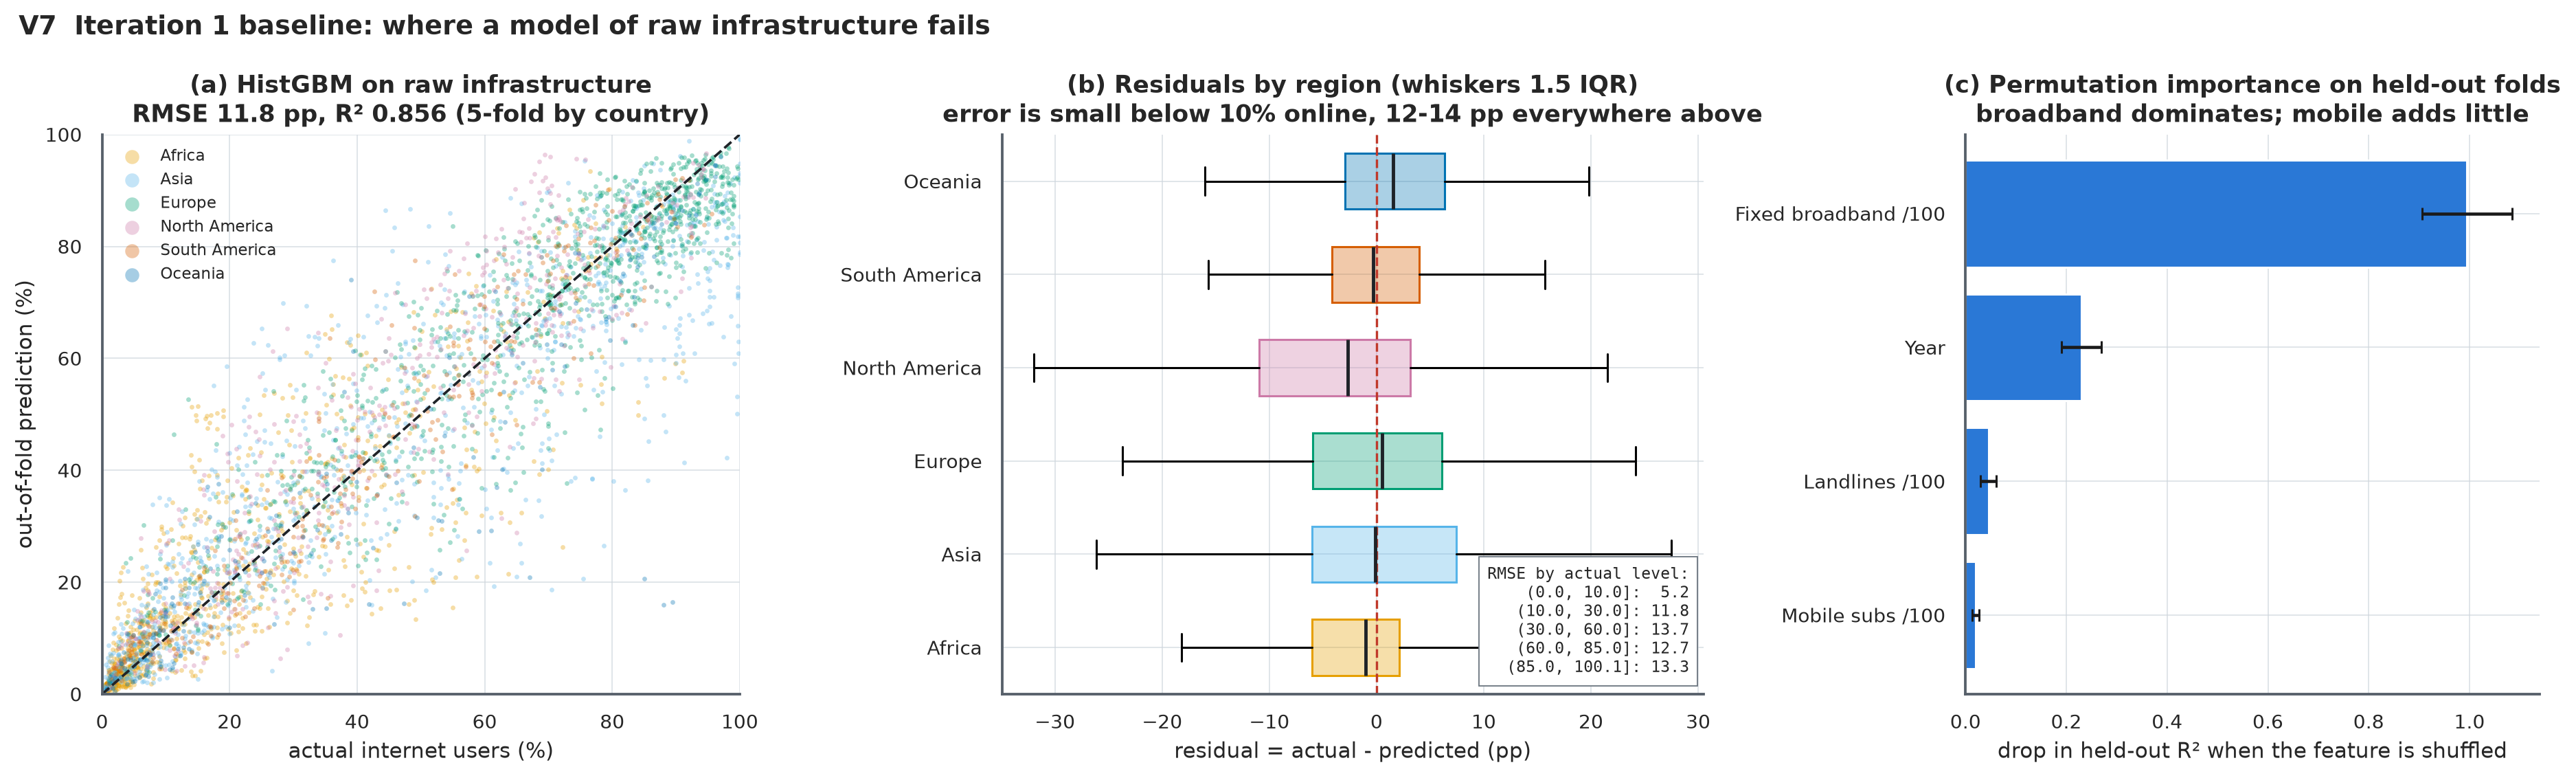
\includegraphics[width=\textwidth]{V7_baseline_diagnostics.png}
\caption{\textbf{V7 (W3, step 1): a raw-infrastructure model explains 86\% of variance but relies on
broadband alone and errs by 12--14 points above 10\% adoption.} (a) Out-of-fold predictions against
actual values. (b) Residuals by region with RMSE by adoption level. (c) Permutation importance on
held-out folds.}
\label{fig:v7}
\end{figure*}

\subsection{Inferences $K_1$ and the feedback loop}
Three inferences leave iteration~1 (W3 rows of Table~\ref{tab:loops}): broadband alone carries the
model, errors are largest where histories differ, and complete cases drop rows that are missing not at
random. The transformation adds 13 past-only features whose definitions come from W1's $K_1$ (history,
per-owner mobile, the broadband floor; V9), and multivariate imputation fitted inside each training
fold with missingness flags, which makes 2{,}134 further rows usable. An inner loop is added in
iteration~2: when the drift chart crosses its threshold, the forecast intervals are re-derived by
conformal calibration.

\subsection{Iteration 2: the transformed model and the forecast}
\textit{Same rows, same folds (Table~\ref{tab:cv}, Fig.~\ref{fig:v10}).} On identical rows (the 4{,}089
complete cases), iteration~2 lowers gradient-boosting RMSE from 11.77 to 10.16 points ($-14\%$; $R^2$
0.856$\rightarrow$0.892). The gain is largest in Asia ($-21\%$), Africa ($-18\%$) and Oceania
($-16\%$), smaller in Europe ($-9\%$) and absent in the Americas ($+1\%$). With MICE, 2{,}134 further
rows become usable (6{,}223 in total) and RMSE reaches 8.84 ($R^2=0.926$). The ablations separate the
two effects: raw features with MICE give 10.67 and engineered features with median imputation give
9.14, so the engineered features carry most of the gain and MICE adds about 0.3.

\begin{table}[!t]
\centering
\caption{Five-fold country-grouped cross-validation (mean $\pm$ s.d.\ over folds)}
\label{tab:cv}
\footnotesize
\begin{tabular}{@{}l r r r@{}}
\toprule
Model (rows) & RMSE & $R^2$ & $n$ \\
\midrule
I1 Ridge, raw (cc) & 13.98$\pm$1.31 & 0.797 & 4089 \\
I1 Random Forest~\cite{breiman2001rf}, raw (cc) & 11.46$\pm$0.50 & 0.863 & 4089 \\
I1 HistGBM~\cite{ke2017lightgbm}, raw (cc) & 11.77$\pm$0.77 & 0.856 & 4089 \\
\textbf{I2 HistGBM, eng.\ + MICE (cc)} & \textbf{10.16$\pm$0.58} & \textbf{0.892} & 4089 \\
\midrule
Abl.\ A: raw + MICE~\cite{vanbuuren2011mice} (all) & 10.67$\pm$0.64 & 0.892 & 6223 \\
Abl.\ B: eng.\ + median (all) & 9.14$\pm$0.71 & 0.920 & 6223 \\
\textbf{I2 HistGBM, eng.\ + MICE (all)} & \textbf{8.84$\pm$0.50} & \textbf{0.926} & 6223 \\
\bottomrule
\multicolumn{4}{@{}l}{\scriptsize cc: complete cases; eng.: engineered features (Table~\ref{tab:loops}).}
\end{tabular}
\end{table}

\begin{figure*}[!t]
\centering
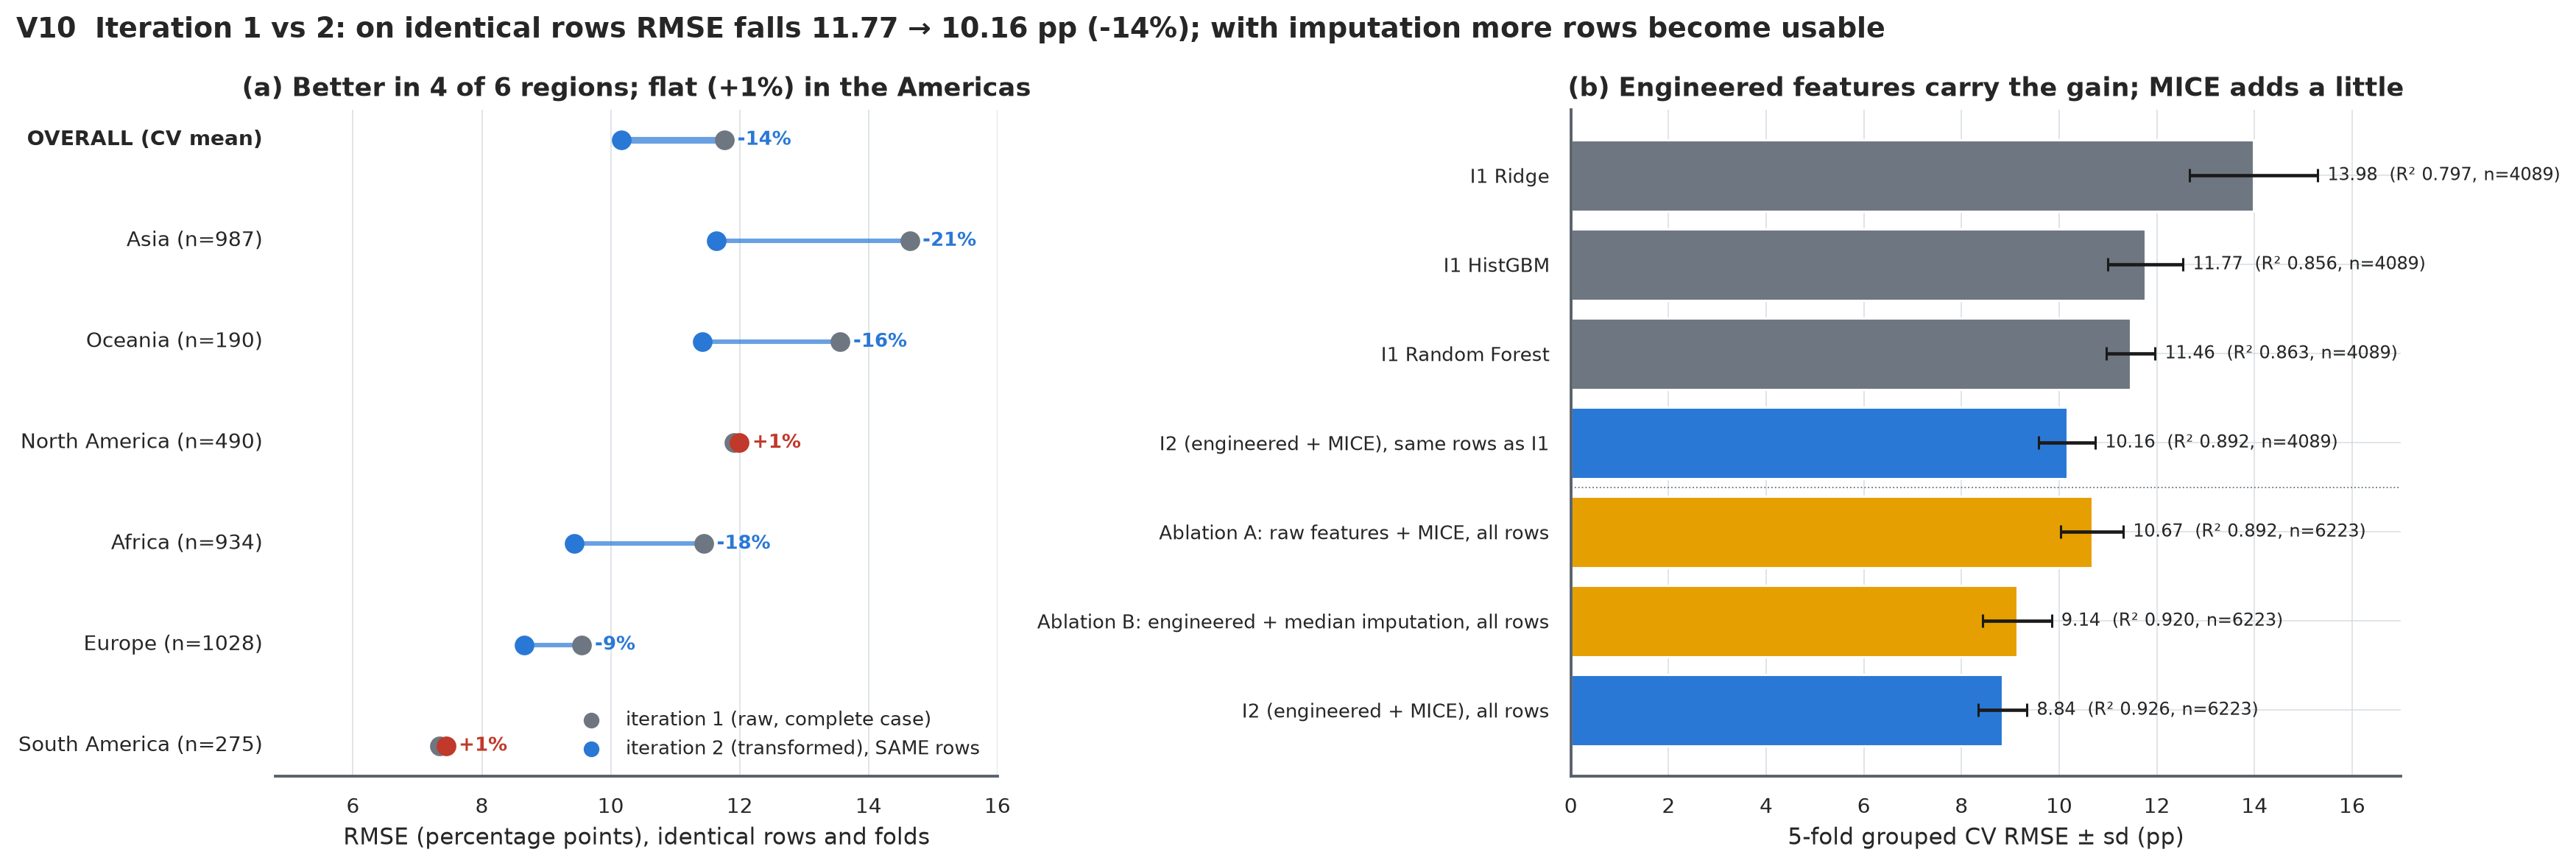
\includegraphics[width=\textwidth]{V10_iteration_comparison.png}
\caption{\textbf{V10 (W3, step 2): on identical rows and folds the transformed data lower error by
14\%, most in Asia and Africa, and engineered features carry most of the gain.} (a) Regional RMSE for
both iterations. (b) All configurations; grey is iteration~1, blue iteration~2, orange the
ablations.}
\label{fig:v10}
\end{figure*}

\textit{Explanation (Figs.~\ref{fig:v11} and~\ref{fig:v12b}a--c).} SHAP values~\cite{lundberg2017shap}
rank phone ownership first, then log broadband, then \texttt{landline\_peak}. Ownership is observed in
only 11\% of rows, so for most rows it is a MICE estimate built from the other indicators and acts as a
composite index rather than a measurement. Partial dependence shows the shape of the learned effects:
predicted internet use is flat while broadband stays on the floor below about 3 per 100 and rises
between 3 and 30 per 100 (a 14-point range); the landline peak adds a further 12 points across its
range, and the years since mobile overtook landlines 5 points. The ICE curves are roughly parallel, so
the effects are mostly additive. The residual map shows where infrastructure under-explains adoption
(blue: the Gulf states, Cuba, Bhutan, Paraguay) and where it over-explains it (red: Mongolia, China,
Egypt, Italy, East Africa). Kosovo's residual of +65 reflects missing data rather than behaviour,
because every infrastructure field is empty for it.

\inference{H3.2 is supported. The model has learned W1's broadband floor and history effect as explicit
shapes, and the remaining residuals have a clear geography, which points to factors outside the dataset
such as policy, price and censorship.}

\begin{figure*}[!t]
\centering
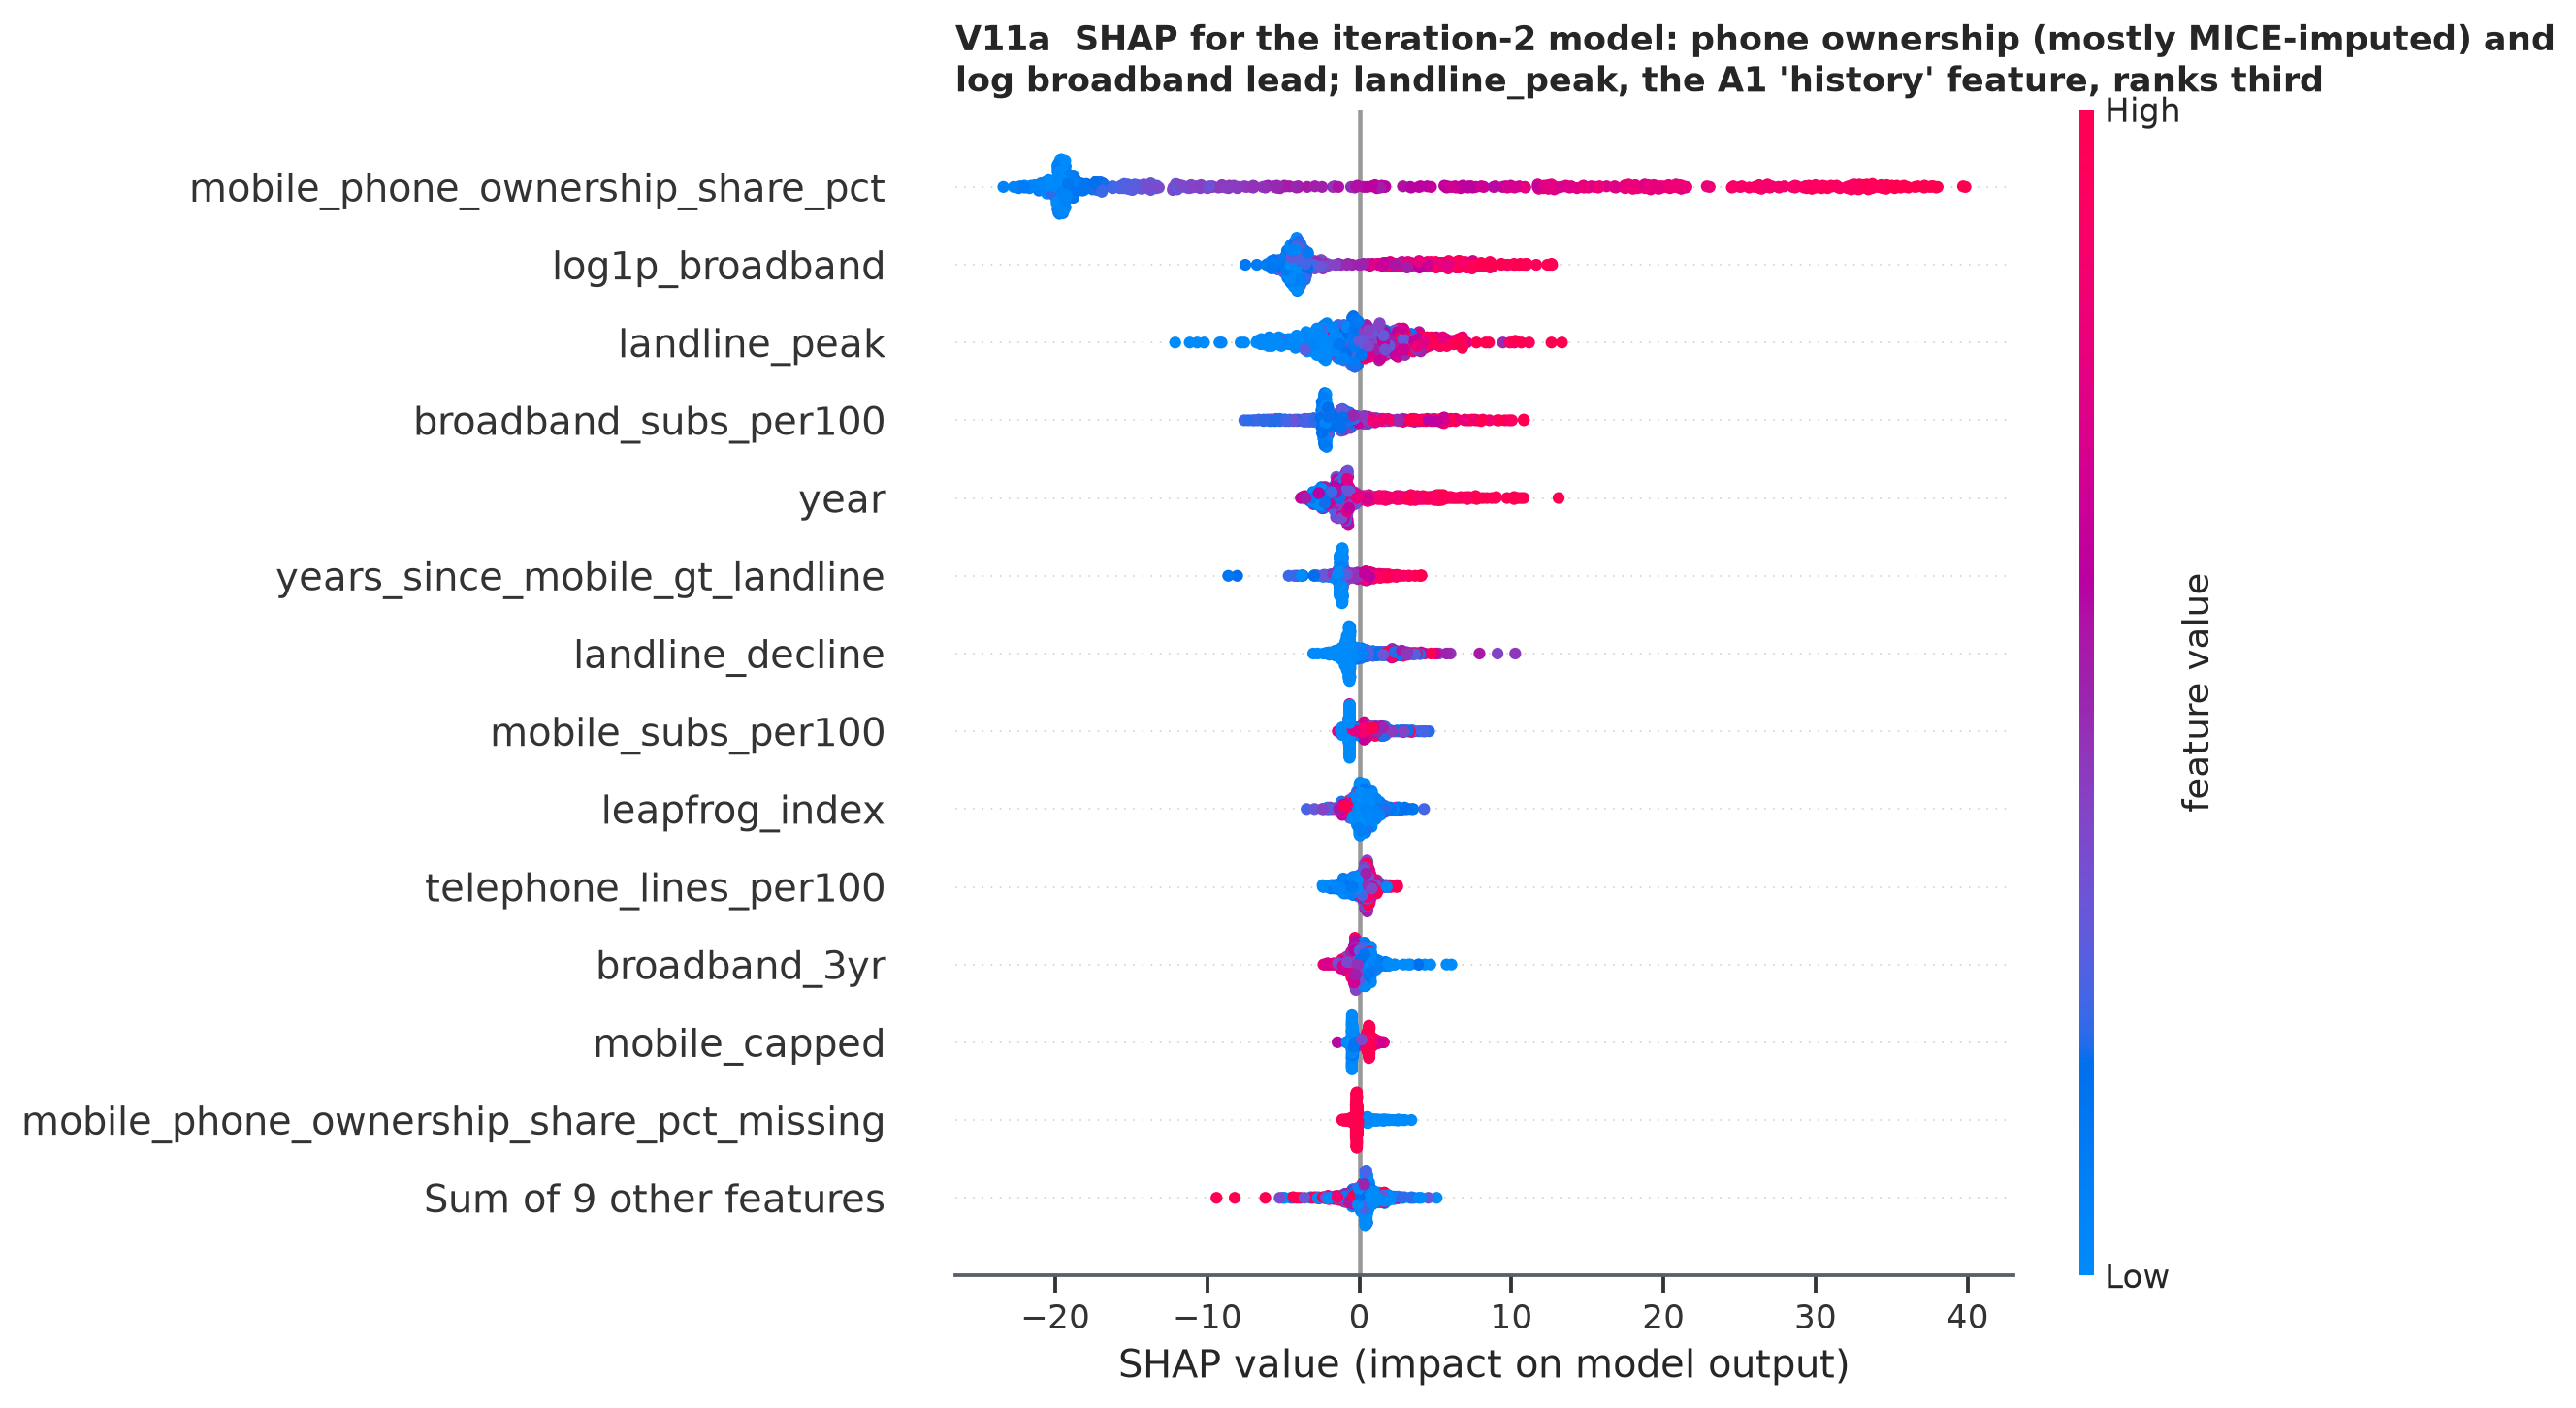
\includegraphics[width=0.40\textwidth]{V11a_shap_beeswarm.png}\hfill
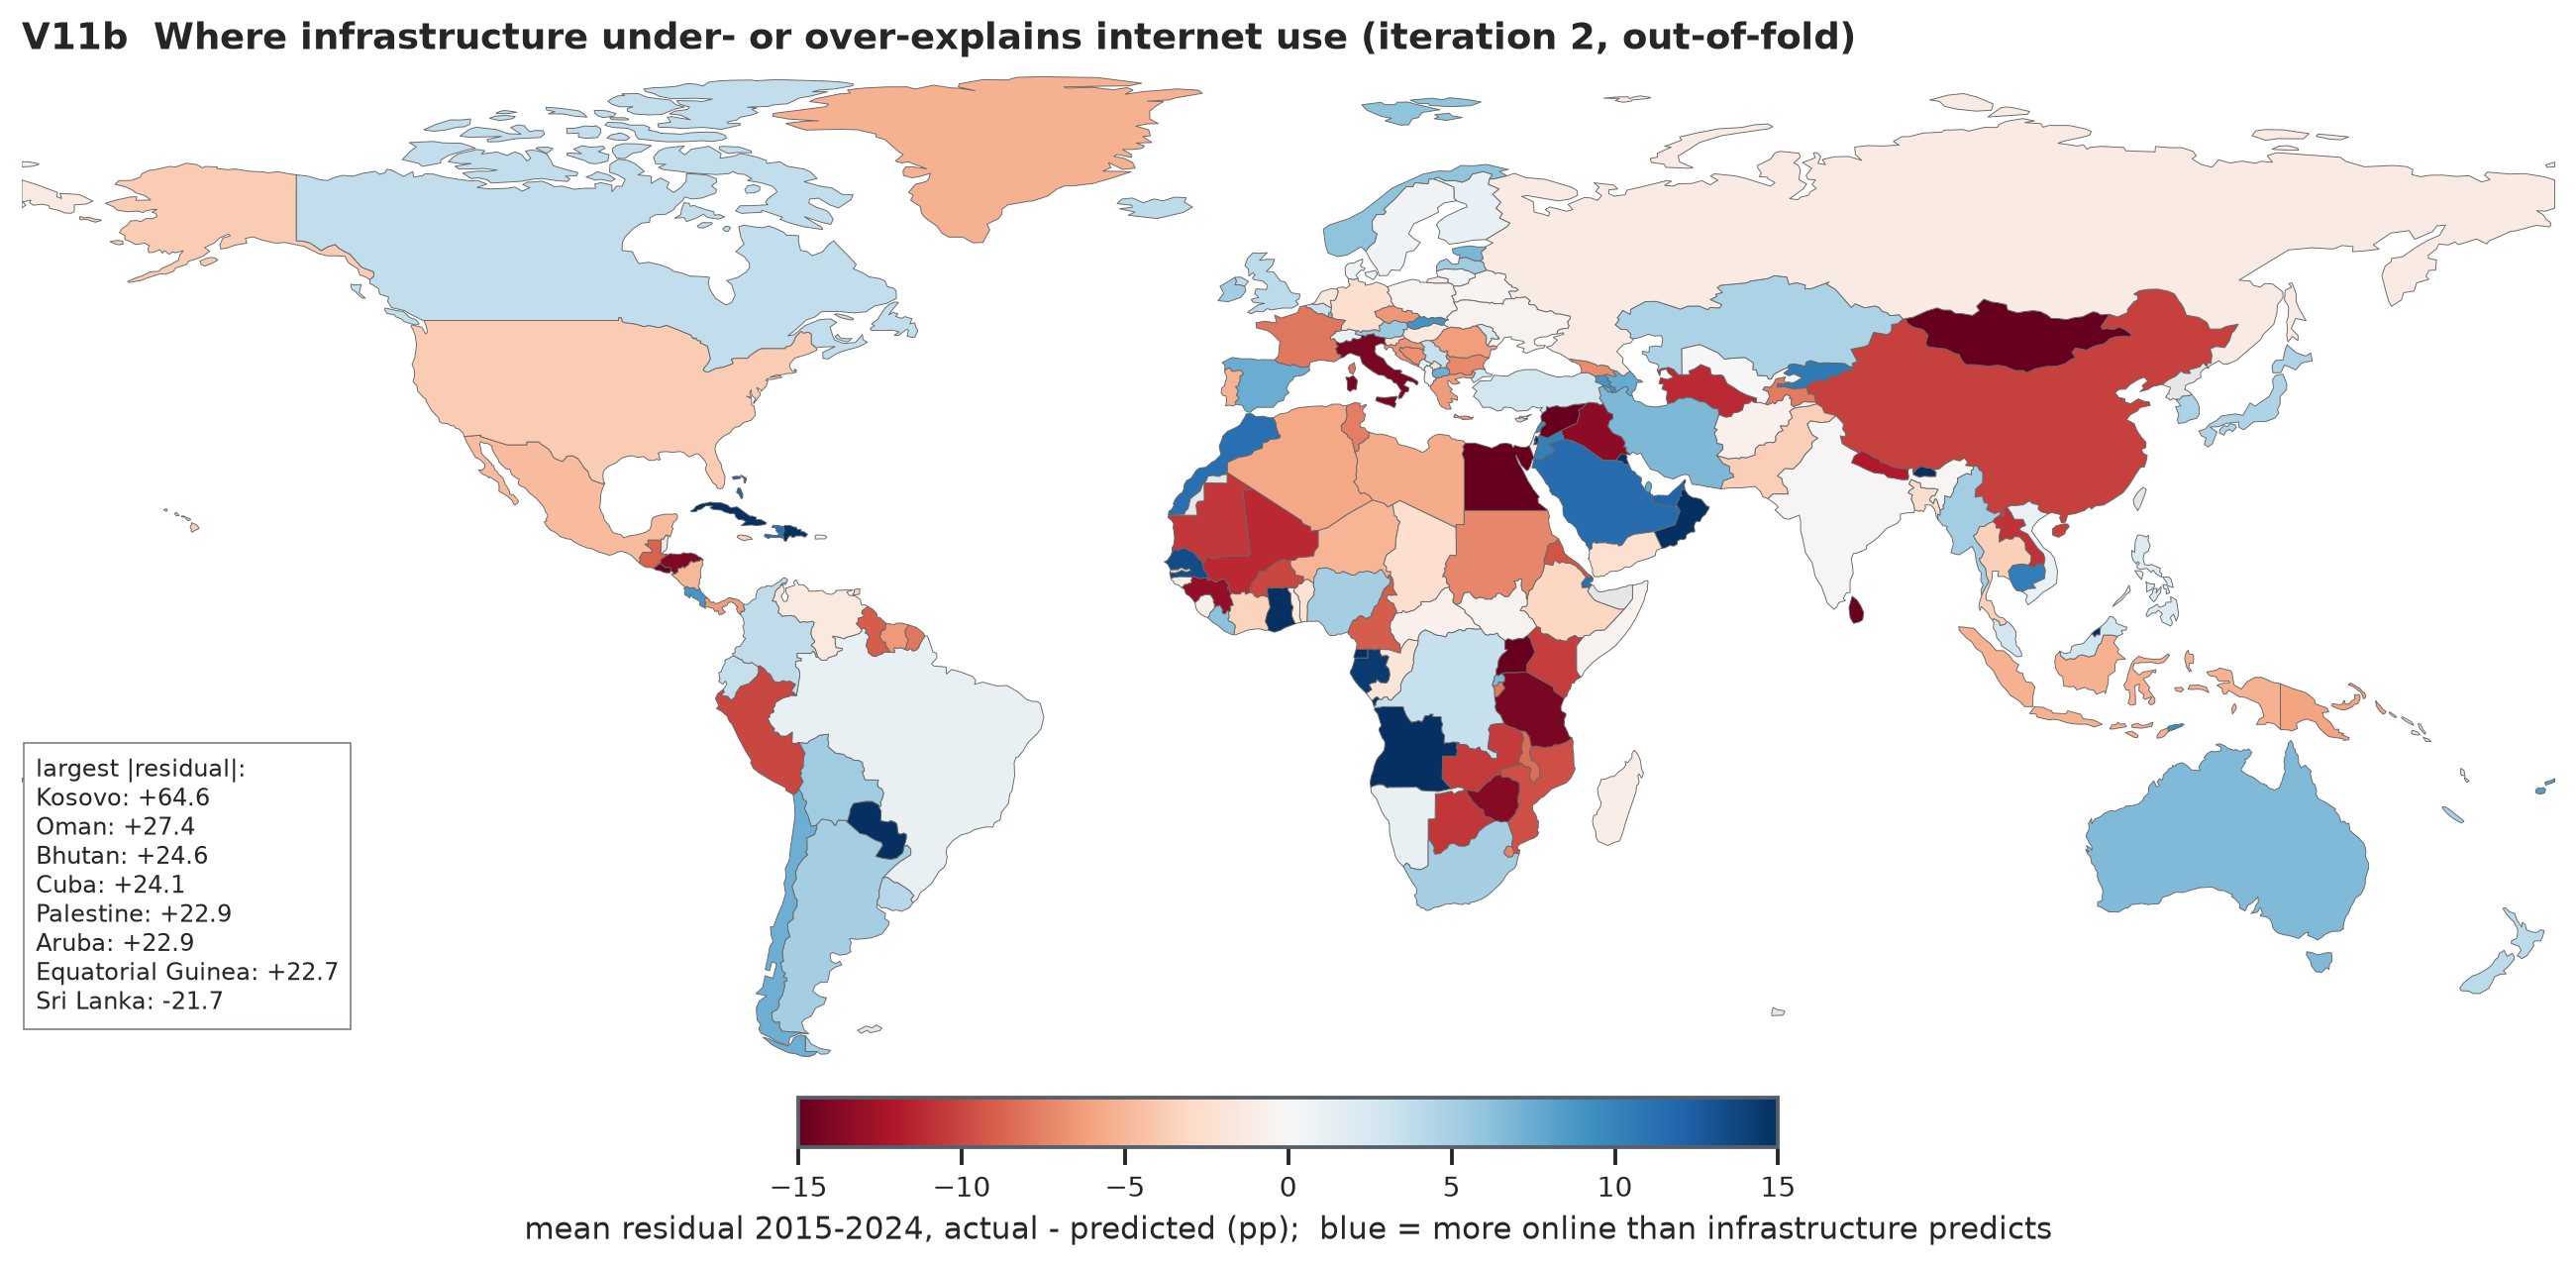
\includegraphics[width=0.58\textwidth]{V11b_residual_choropleth.png}
\caption{\textbf{V11 (W3, step 3): imputed ownership, broadband and the landline peak drive the model,
and its remaining errors are geographically clustered.} (a) SHAP beeswarm over 600 sampled rows.
(b) Mean out-of-fold residual for 2015--2024 per country; an interactive version is in
\texttt{outputs/} and the demonstrator.}
\label{fig:v11}
\end{figure*}

\textit{Drift (Fig.~\ref{fig:v13}).} After 2020 the target crosses the 0.2 threshold (mean PSI 0.44 in
2022--2024) while every input stays below 0.2 until 2023. The same infrastructure now coincides with
more internet use, so the input-to-output relationship has shifted, which is concept drift in the sense
of Gama et~al.~\cite{gama2014}. A model trained up to 2020 cannot know this, and its forecasts should be
expected to be too low and too confident.

\begin{figure*}[!t]
\centering
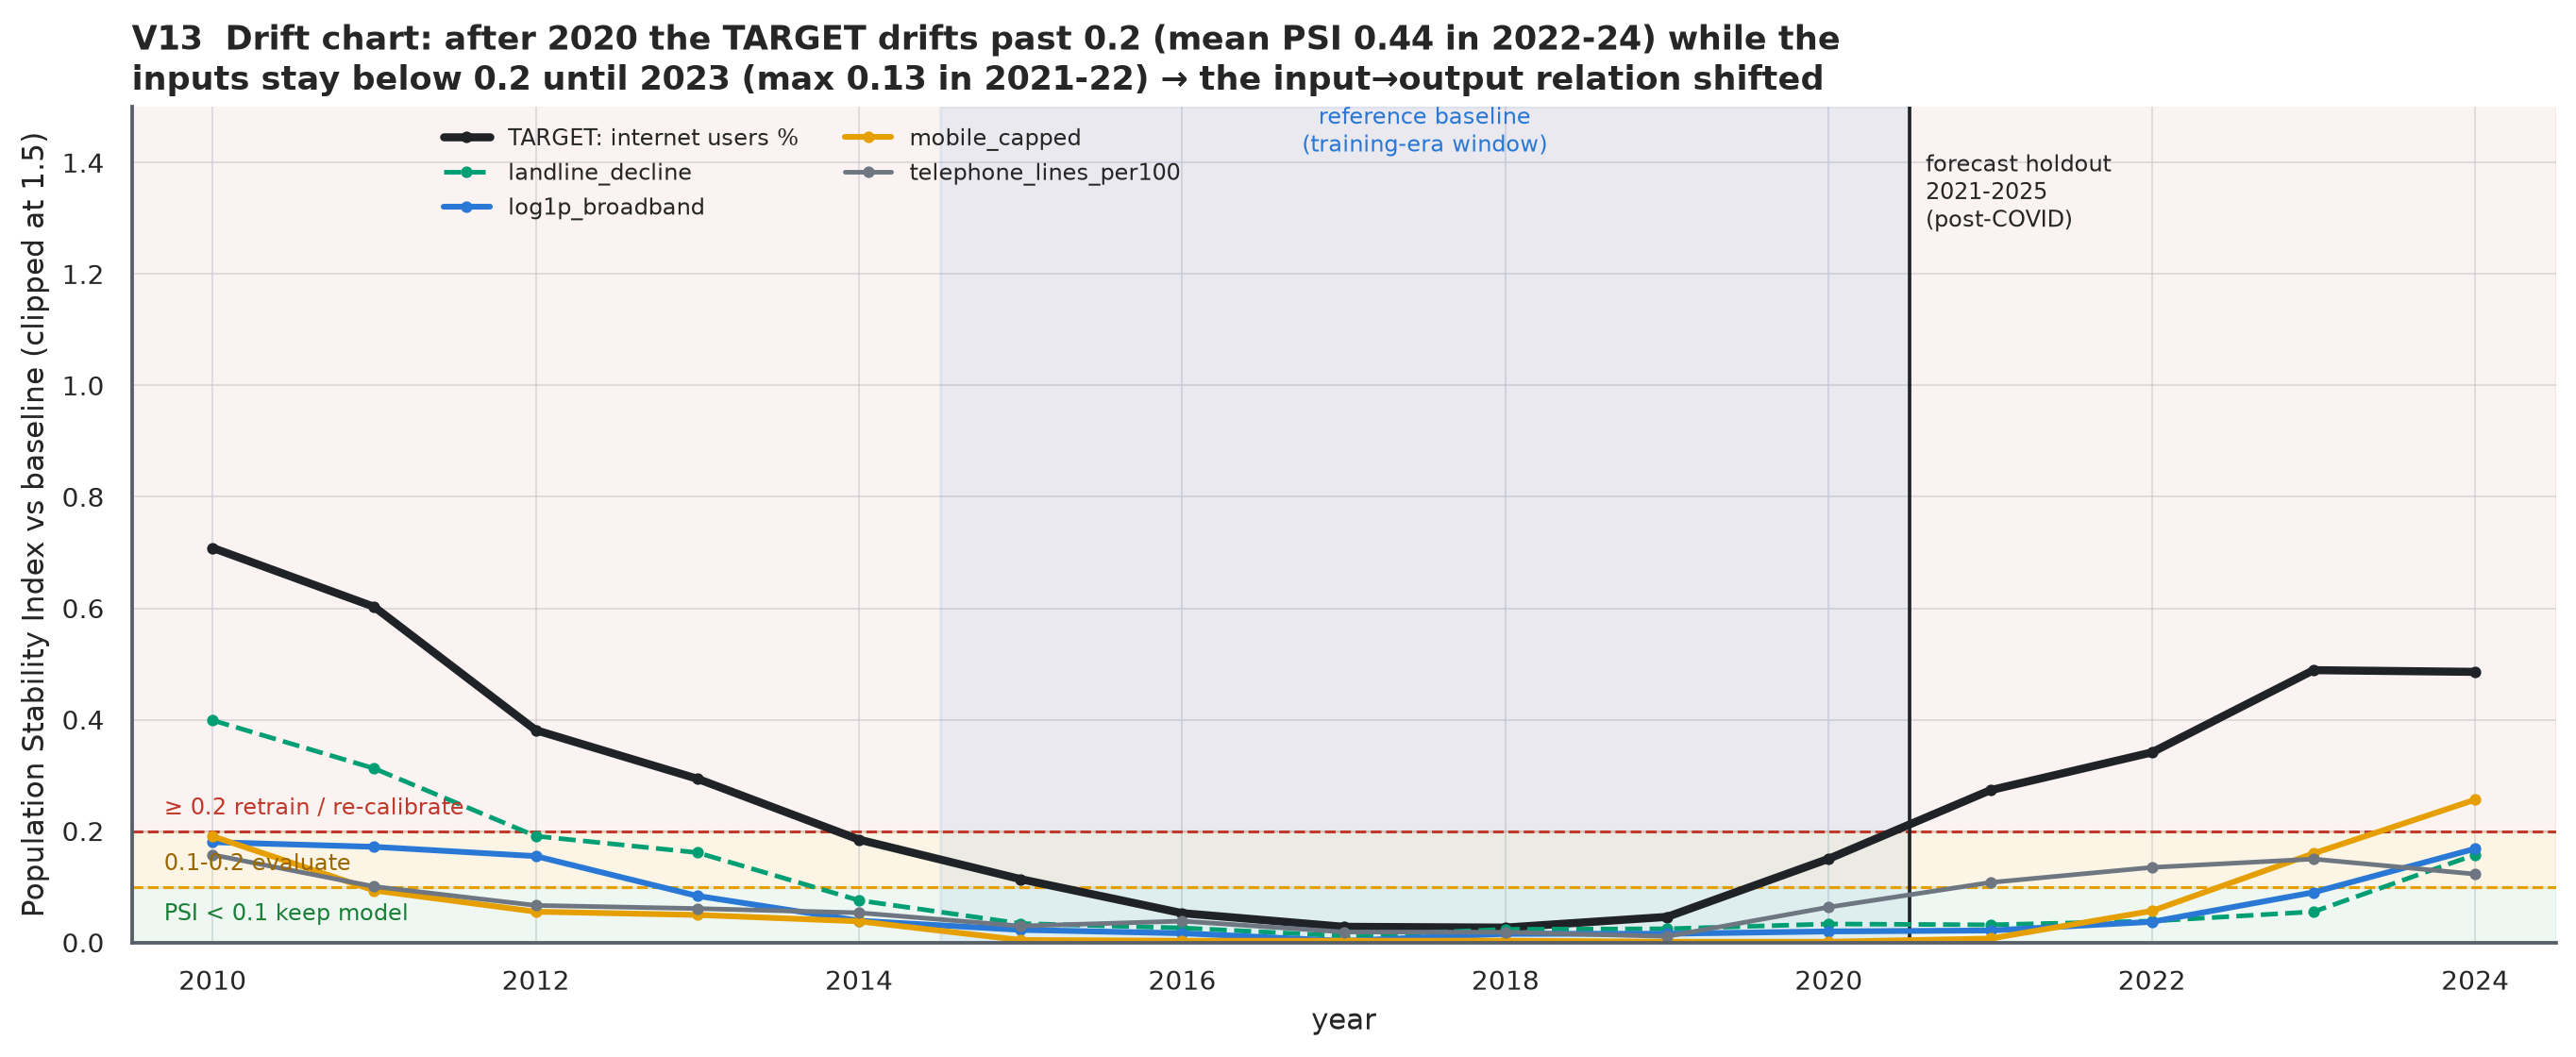
\includegraphics[width=0.92\textwidth]{V13_psi_drift_chart.png}
\caption{\textbf{V13 (W3, step 5): after 2020 the target drifts past the retraining threshold while
the inputs do not.} PSI against the 2015--2020 baseline for the target (black) and the main features,
with action thresholds. Ownership-based features are omitted because too few countries report them per
year for a stable PSI.}
\label{fig:v13}
\end{figure*}

\textit{Forecast (Fig.~\ref{fig:v12}).} Quantile gradient boosting trained on years up to 2020
forecasts 735 country-years in 2021--2025 with an RMSE of 10.1 points ($R^2=0.84$). As the drift chart
anticipates, the errors are one-sided: 71\% of forecasts are too low (mean error +4.9 points) and the
nominal 80\% interval covers only 50\% of outcomes. CQR widens the interval by 4.7 points and restores
83\% coverage (78--93\% in each year with $n\ge180$; 2025 has only ten rows). The calibration curve
(Fig.~\ref{fig:v12b}d) repeats the test at five nominal levels: the raw intervals cover 27, 37, 45, 50
and 68\% at nominal 50--90\%, whereas CQR covers 50, 62, 74, 83 and 94\%, within four points of the
diagonal at every level.

\inference{H3.3 is rejected for the raw model and recovered by the inner loop: uncertainty must be
re-calibrated whenever the drift chart crosses its threshold, and the conformal cone then matches
observed outcomes at every level.}

\begin{figure*}[!t]
\centering
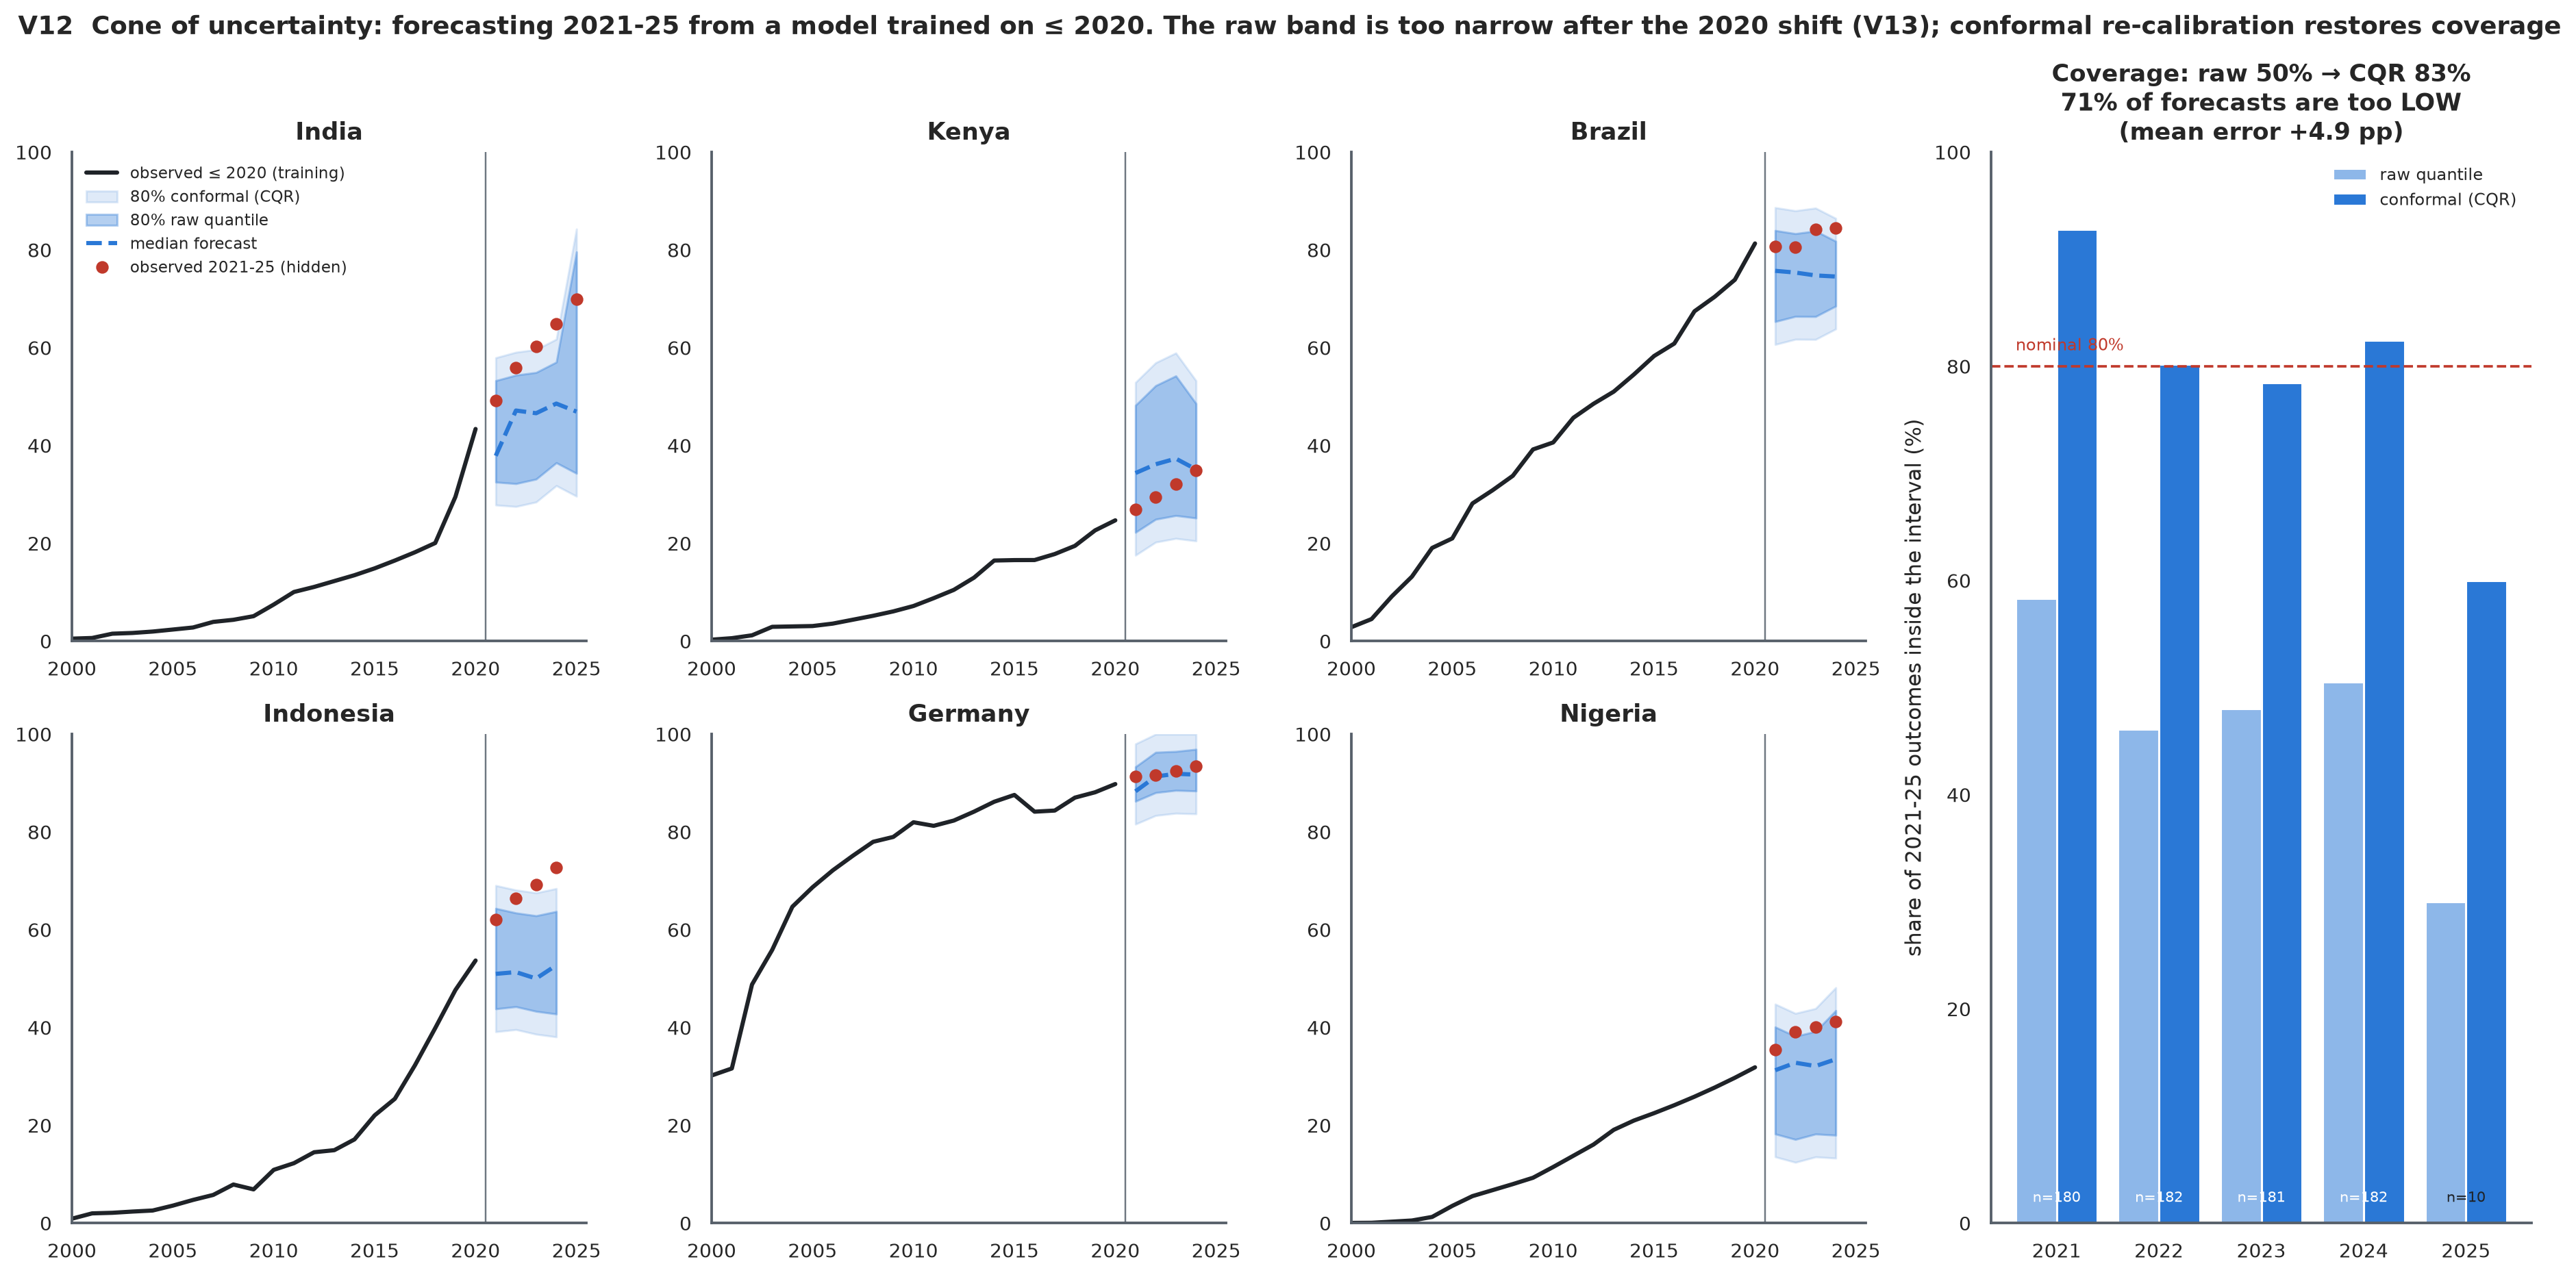
\includegraphics[width=\textwidth]{V12_forecast_fan_chart.png}
\caption{\textbf{V12 (W3, step 6): forecasts made in 2020 are too low after the shift, and conformal
re-calibration restores the nominal coverage.} Six countries: training data (black), median forecast
(dashed), raw 80\% quantile band (dark), conformal band (light) and the hidden 2021--2025 outcomes
(red). Right: coverage per year.}
\label{fig:v12}
\end{figure*}

\begin{figure*}[!t]
\centering
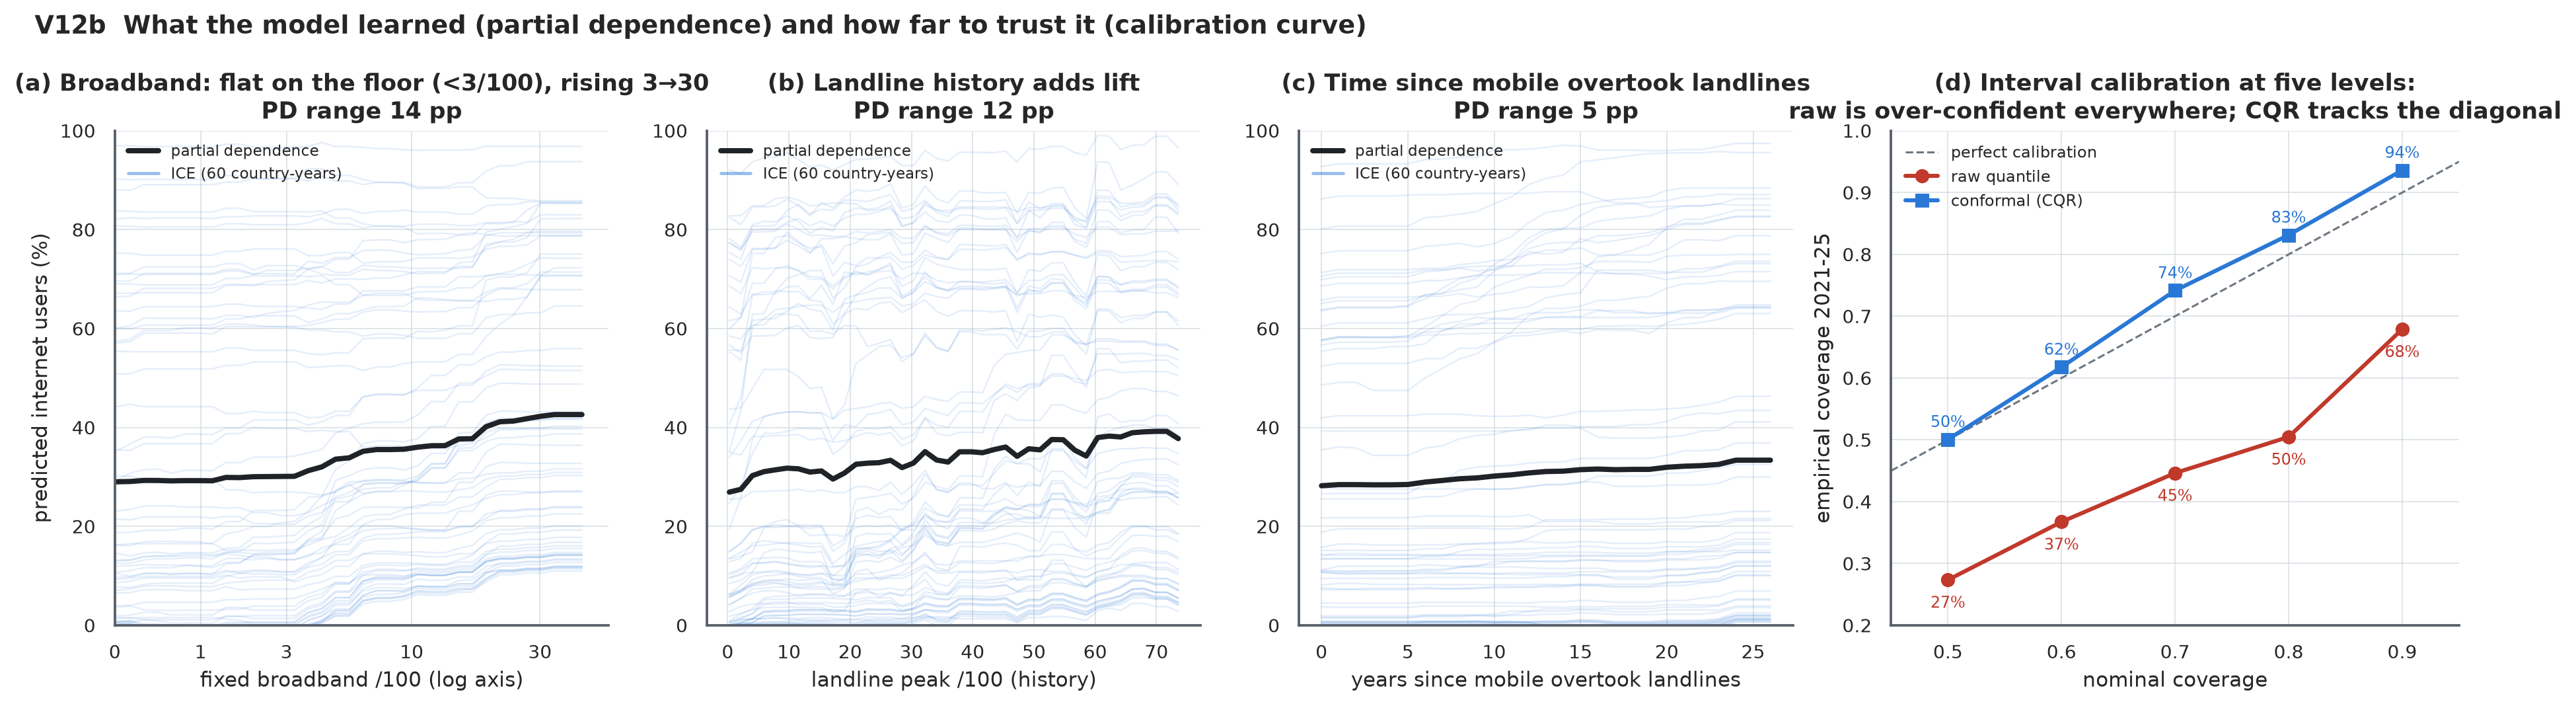
\includegraphics[width=\textwidth]{V12b_pdp_calibration.png}
\caption{\textbf{V12b (W3, steps 4 and 6): the model has learned the broadband floor and a history
effect, and only the conformal intervals are calibrated.} (a--c) Partial dependence (black) and 60 ICE
curves (blue) for log broadband, landline peak and years since mobile overtook landlines. (d) Empirical
coverage in 2021--2025 against nominal coverage for raw and conformal intervals.}
\label{fig:v12b}
\end{figure*}

\subsection{Knowledge $K_2$ and the analysis path}
History lowers error by 14\% on identical rows, most in Asia and Africa, through effects that can be
read directly; after 2020 the relation between infrastructure and use has shifted, and only
re-calibrated intervals can be trusted. \textit{Analysis path.} The baseline diagnostics (V7) set the
inferences; after $T$, the iteration comparison (V10) measured the gain on identical rows, SHAP and the
residual map (V11) explained it and located the remaining error, partial dependence (V12b a--c) showed
the learned shapes, the drift chart (V13) was read before the forecast, and the fan chart and
calibration curve (V12, V12b d) tested the re-calibrated intervals. The result enters the synthesis
(V14b, d).

% =========================================================================================
\section{Synthesis and Discussion}\label{sec:disc}
% =========================================================================================
\subsection{Knowledge $K^\ast$: answering the main question}\label{sec:k2}
Fig.~\ref{fig:v14} assembles the answer from the three workflows. Diffusion followed one S-curve
everywhere but took off 6--12 years later outside Europe, and late starters did not climb faster
(W1; panel a). In the 2023 cross-section, broadband ($\rho=0.79$) and the landline peak (0.81)
separate countries, whereas mobile, raw or capped, reaches only 0.52--0.53 and SIMs per owner 0.00
(W1, W3; panel b). Mobile is saturated (capped median 100 per 100) in both the majority and the
early-saturating archetypes, and late starters trail at 79, whereas fixed infrastructure separates all
three, with median broadband of 0, 17 and 40 per 100 (W2; panel c). Every feedback loop improved the
quantity it could be checked on: error on the same rows, cluster separation and interval coverage
(panel d).

W1's direct test agrees: the 22 countries that skipped landlines and saturated on mobile have a median
of 44\% online, against 93\% where landlines were built (V1f). The answer to A1's question is therefore
that mobile leapfrogging happened but did not close the divide. The divide is a delay on a common S-curve; it is narrowing in relative terms but not
closing in absolute terms; and fixed infrastructure, not mobile saturation, marks where a country
stands on the curve.

\begin{figure*}[!t]
\centering
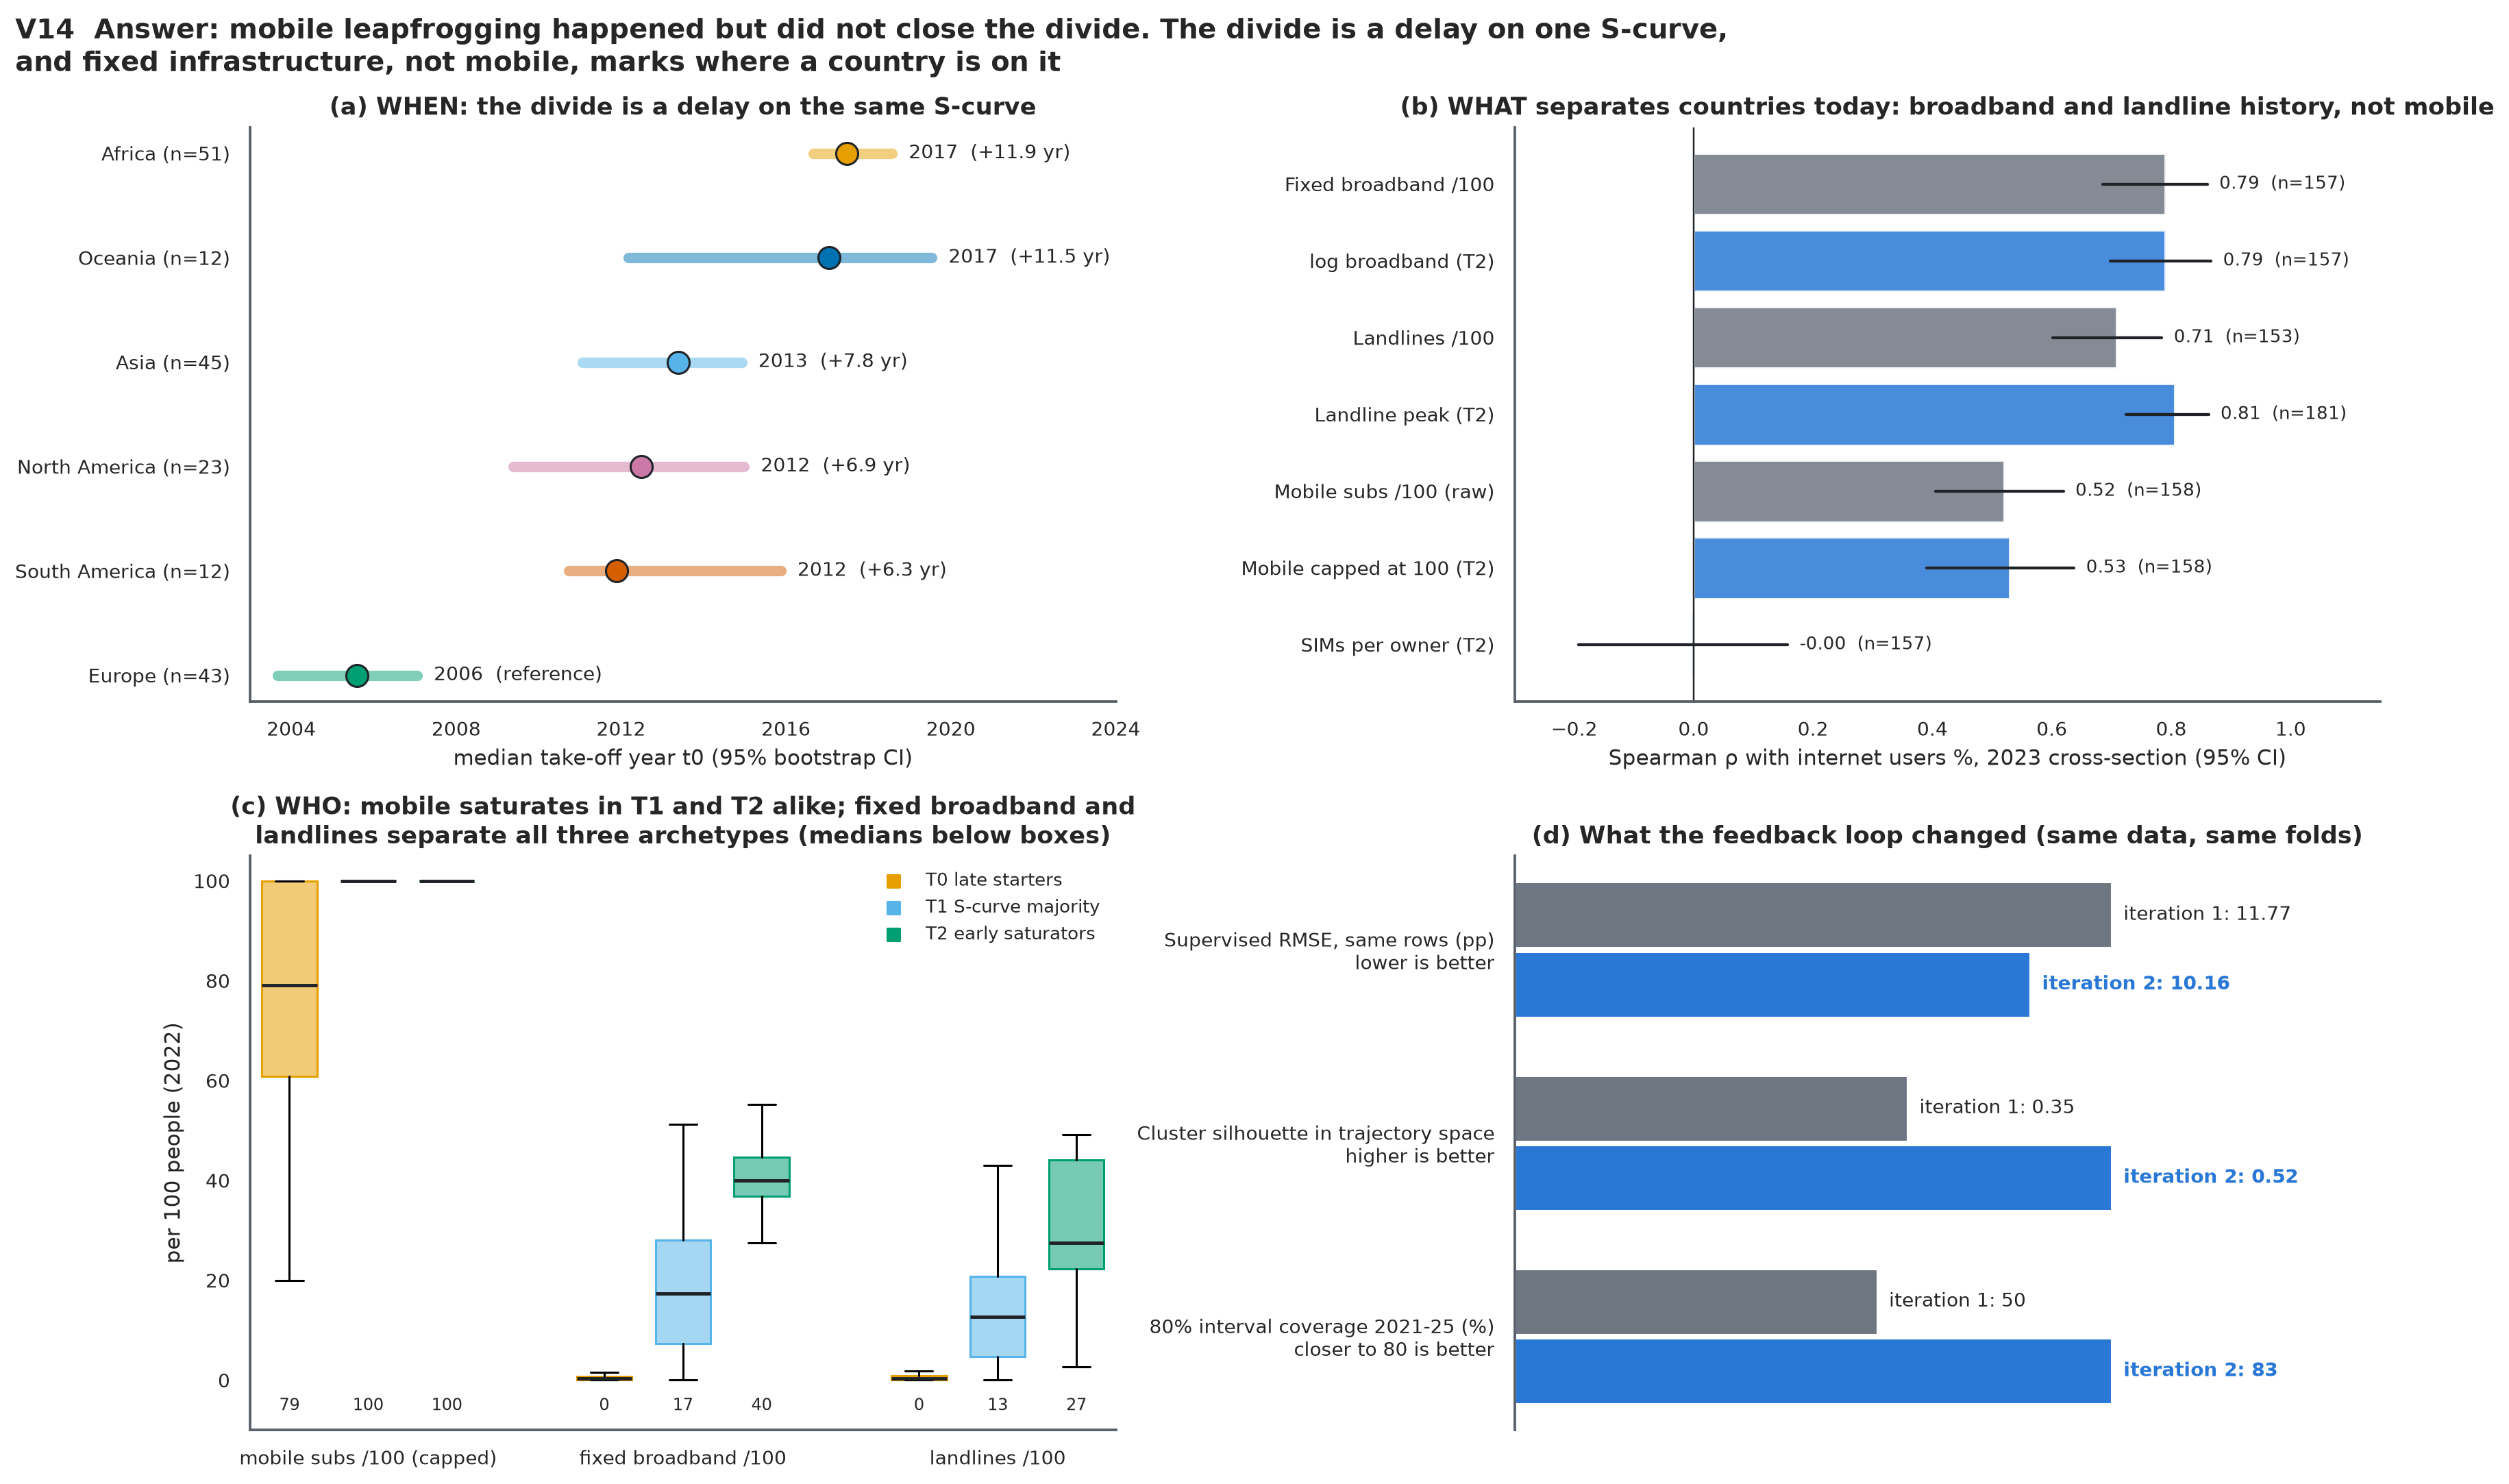
\includegraphics[width=\textwidth]{V14_synthesis_answer.png}
\caption{\textbf{V14 (synthesis $K^\ast$): the divide is a delay on one S-curve, and fixed
infrastructure rather than mobile marks a country's position on it.} (a) Median take-off year by region
with bootstrap intervals (W1). (b) Spearman $\rho$ with internet use in 2023 for raw (grey) and
transformed (blue) features (W1, W3). (c) Mobile, broadband and landlines in 2022 by trajectory
archetype (W2). (d) Iteration~1 against iteration~2 on three checks (W2, W3).}
\label{fig:v14}
\end{figure*}

\subsection{A1's visual claims, re-tested}
Table~\ref{tab:a1} lists each A1 claim, the A3 test applied to it and the verdict. Five of six are
confirmed and quantified; one, that the gap kept widening, is refined, because the A3 data show the
absolute gap peaking in 2014.

\begin{table*}[!t]
\centering
\caption{A1's visual claims re-tested in A3}
\label{tab:a1}
\footnotesize
\begin{tabularx}{\textwidth}{@{}Y Y Y l l@{}}
\toprule
A1 claim (appendix figure) & A3 test & Result & Workflow & Verdict \\
\midrule
Regions are years behind Europe (Fig.~14) & logistic $t_0$, Kruskal--Wallis, Holm-corrected Mann--Whitney; alignment (V1, V1c) & Africa +11.9 yr, $p=10^{-15}$; aligned spread 32$\rightarrow$10 pp & W1 & confirmed \\
The gap widened (Fig.~11) & $\sigma$-convergence, Gini, regional gap, headroom (V1e) & absolute gap peaked 2014 (64 pp), now 52; Gini 0.81$\rightarrow$0.19 & W1 & refined \\
Broadband matters more than mobile (Figs.~19--20) & bootstrap Spearman by year; permutation importance; partial dependence (V2, V7, V12b) & 0.80 vs 0.42 in 2024; mobile importance 0.02 & W1, W3 & confirmed \\
Subscriptions are not people (Figs.~10, 18) & SIMs per owner; anomaly persistence (V3, V6b) & median 1.34 SIMs per owner; Fiji transient & W1, W2 & confirmed \\
Same level today, opposite histories (Fig.~5) & DTW trajectory clusters vs snapshot clusters (V8, V8d) & 37 of 133 regrouped; silhouette 0.52 vs 0.35 & W2 & confirmed \\
Mobile let countries skip fixed lines (A1 conclusion) & leapfroggers vs landline builders, Mann--Whitney; Spearman within Africa (V1f) & 44\% vs 93\% online, $p=10^{-11}$; $\rho=0.86$ within Africa & W1 & refined: skipped, not caught up \\
Four kinds of country (Fig.~23) & $k$-means/GMM/Ward with stability (V5, V5b) & three archetypes, ARI 0.64, 15 border countries & W2 & confirmed, weaker \\
\bottomrule
\end{tabularx}
\end{table*}

\subsection{What the second iterations learned}
Each second iteration added something the first could not provide. W1's re-expression in own time
showed that the regional differences are differences of timing on one shape, and headroom showed that
the furthest behind close least. W2's trajectories showed that archetypes are defined by paths: they
are better separated (0.52 against 0.35), regroup 37 of 133 countries and are ordered by timing. W3's
history features improved prediction for countries the model has never seen, most in Asia and Africa,
and its drift chart flagged the post-2020 shift before the forecast errors confirmed it.

\subsection{Threats to validity}
\textit{Internal validity.} Leakage is controlled by country-grouped folds, past-only features,
in-fold imputation, a temporal holdout and an automated guard. The comparison between iterations
uses the same rows and folds, so the 14\% gain is not an artefact of different samples. The alignment
of V1c uses parameters fitted to the same curves, so its evidence is the common shape across regions
rather than the size of the collapse. \textit{External validity.} Results describe country-level
averages; sub-national divides (urban against rural) are invisible in the data. \textit{Construct
validity.} ``Internet user'' is a survey-based ITU definition whose recall window varies across
countries~\cite{itu2023}, and subscriptions count SIM cards rather than people (V3). \textit{Conclusion
validity.} Many tests are run; the regional comparisons are Holm-corrected, and every interval is a
bootstrap or a conformal interval rather than a normal approximation.

\subsection{Limitations}\label{sec:limits}
\begin{itemize}
\item \textit{Association, not cause.} No income variable is used, by design, so national wealth
  may drive both infrastructure and use; no causal effect is identified.
\item \textit{Missing not at random.} Ownership and broadband are missing mostly for less-connected
  country-years (Mann--Whitney $p=10^{-41}$). MICE with missingness flags reduces this bias without removing it, and
  imputed ownership dominates SHAP for this reason.
\item \textit{Moderate stability.} Snapshot clusters reach a bootstrap ARI of 0.64 and are reported
  as a description of 2024, not as a taxonomy.
\item \textit{Heuristic artefact rules.} The rules are conservative (ten cells) and every removal is
  listed in \texttt{outputs/p1\_artifact\_log.csv}; the persistence classes of V6b use fixed thresholds.
\item \textit{Exchangeability.} Conformal coverage assumes it, and drift violates it; a larger shift
  after 2024 would require re-calibration again.
\item \textit{Logistic extrapolation.} Saturation levels are poorly identified for countries still
  before their inflection point, so $L$ is not interpreted for late starters.
\end{itemize}

\subsection{Reproducibility and system architecture}\label{sec:repro}
A single module (\texttt{src/common.py})
defines the panel, regions, thresholds, artefact rules and engineered features, so the shared parts of
the feedback loops have one definition. Three groups of analysis modules, one per workflow, write tables
and figures; the workflow diagrams are generated from those figures; and the report, the deck and the
application only read the generated artefacts. Every figure and number is produced by
\texttt{python src/run\_all.py} and \texttt{python src/build\_diagrams.py} in about five minutes with
fixed seeds.

The interactive
demonstrator runs locally (\texttt{streamlit run app.py}) or in a web browser without installation
through a WebAssembly build of the same application.

% =========================================================================================
\section{Conclusion and Future Work}
% =========================================================================================
Three unrolled workflows, each with written hypotheses, plugged-in visual evidence, a recorded path and
one feedback loop that transforms the data, turned A1's visual impressions into tested inferences.
Every second iteration improved on its first: aligned curves collapsed, trajectory archetypes separated
better, prediction error fell on identical rows and re-calibrated intervals matched their nominal
coverage. Mobile leapfrogging did not close the digital divide: the divide is a delay of 6--12 years on
a shared S-curve, it is narrowing only in relative terms, late starters close the smallest share of
their remaining gap, and fixed infrastructure, not mobile, marks where a country stands.

Three extensions follow directly. Affordability data (the price of a mobile-broadband basket as a
share of income) would test whether the residual geography of V11 reflects price. Sub-national data
would expose the urban--rural divide hidden by country averages. A third iteration with a
drift-triggered retraining rule (retrain when PSI exceeds 0.2) would close W3's inner loop
automatically rather than by analyst inspection.

% =========================================================================================
\section*{Individual Contributions}
\begin{table}[!h]
\centering
\footnotesize
\begin{tabularx}{\columnwidth}{@{}l Y@{}}
\toprule
Member & Contribution \\
\midrule
Parikshith & Workflow W1 (statistical analysis): logistic diffusion fits, rank tests, convergence and
headroom analysis, alignment in own time, segmented regression, bootstrap correlations, data-quality and
missingness analysis, take-off map and leapfrog test (V1, V1c, V1d, V1e, V1f, V2, V3); shared transformation core with artefact rules and
engineered features (V9); main question, workflow diagrams and system architecture (V0, W1--W3);
synthesis (V14); integration and report \\
Sindhoor & Workflow W2 (unsupervised mining): PCA; $k$-means, GMM and Ward clustering with $k$-selection,
bootstrap co-assignment and silhouette analysis; Isolation Forest and LOF anomalies with per-year
persistence and deviation profiles (V4, V5, V5b, V6, V6b, V6c); DTW trajectory clustering,
dendrogram, timing and iteration comparison (V8, V8a, V8d) \\
Varshith & Workflow W3 (supervised learning): leakage guards; Ridge, Random Forest and gradient-boosting
models with ablations (V7, V10); SHAP and residual map (V11); PSI drift chart (V13); quantile forecast
with conformal re-calibration, partial dependence and calibration curve (V12, V12b); browser
demonstrator \\
\bottomrule
\end{tabularx}
\end{table}

\begin{thebibliography}{99}
\bibitem{keim2008scope} D.~A. Keim, F.~Mansmann, J.~Schneidewind, J.~Thomas, and H.~Ziegler,
``Visual analytics: Scope and challenges,'' in \emph{Visual Data Mining}, LNCS 4404. Berlin, Germany: Springer, 2008, pp.~76--90.
\bibitem{keim2008challenges} D.~Keim, G.~Andrienko, J.-D. Fekete, C.~G\"org, J.~Kohlhammer, and
G.~Melan\c{c}on, ``Visual analytics: Definition, process, and challenges,'' in \emph{Information
Visualization}, LNCS 4950. Berlin, Germany: Springer, 2008, pp.~154--175.
\bibitem{card1999} S.~K. Card, J.~D. Mackinlay, and B.~Shneiderman, Eds., \emph{Readings in
Information Visualization: Using Vision to Think}. San Francisco, CA, USA: Morgan Kaufmann, 1999.
\bibitem{sacha2014} D.~Sacha, A.~Stoffel, F.~Stoffel, B.~C. Kwon, G.~Ellis, and D.~A. Keim,
``Knowledge generation model for visual analytics,'' \emph{IEEE Trans. Vis. Comput. Graphics},
vol.~20, no.~12, pp.~1604--1613, 2014.
\bibitem{wang2024va4ml} J.~Wang, S.~Liu, and W.~Zhang, ``Visual analytics for machine learning: A
data perspective survey,'' \emph{IEEE Trans. Vis. Comput. Graphics}, vol.~30, no.~12, pp.~7637--7656, 2024.
\bibitem{javed2012composite} W.~Javed and N.~Elmqvist, ``Exploring the design space of composite
visualization,'' in \emph{Proc. IEEE Pacific Vis. Symp.}, 2012, pp.~1--8.
\bibitem{munzner2014} T.~Munzner, \emph{Visualization Analysis and Design}. Boca Raton, FL, USA: CRC Press, 2014.
\bibitem{owid} H.~Ritchie, E.~Mathieu, M.~Roser, and E.~Ortiz-Ospina, ``Internet,'' Our World in
Data, 2023. [Online]. Available: \url{https://ourworldindata.org/internet}
\bibitem{itu2023} International Telecommunication Union, \emph{Measuring Digital Development: Facts
and Figures 2023}. Geneva, Switzerland: ITU, 2023.
\bibitem{rogers2003} E.~M. Rogers, \emph{Diffusion of Innovations}, 5th~ed. New York, NY, USA: Free Press, 2003.
\bibitem{comin2010} D.~Comin and B.~Hobijn, ``An exploration of technology diffusion,''
\emph{Amer. Econ. Rev.}, vol.~100, no.~5, pp.~2031--2059, 2010.
\bibitem{kruskal1952} W.~H. Kruskal and W.~A. Wallis, ``Use of ranks in one-criterion variance
analysis,'' \emph{J. Amer. Statist. Assoc.}, vol.~47, no.~260, pp.~583--621, 1952.
\bibitem{holm1979} S.~Holm, ``A simple sequentially rejective multiple test procedure,''
\emph{Scand. J. Statist.}, vol.~6, no.~2, pp.~65--70, 1979.
\bibitem{cleveland1979} W.~S. Cleveland, ``Robust locally weighted regression and smoothing
scatterplots,'' \emph{J. Amer. Statist. Assoc.}, vol.~74, no.~368, pp.~829--836, 1979.
\bibitem{efron1993} B.~Efron and R.~J. Tibshirani, \emph{An Introduction to the Bootstrap}.
New York, NY, USA: Chapman \& Hall, 1993.
\bibitem{jolliffe2016} I.~T. Jolliffe and J.~Cadima, ``Principal component analysis: A review and
recent developments,'' \emph{Phil. Trans. R. Soc. A}, vol.~374, no.~2065, 2016, Art.~no.~20150202.
\bibitem{rousseeuw1987} P.~J. Rousseeuw, ``Silhouettes: A graphical aid to the interpretation and
validation of cluster analysis,'' \emph{J. Comput. Appl. Math.}, vol.~20, pp.~53--65, 1987.
\bibitem{hubert1985} L.~Hubert and P.~Arabie, ``Comparing partitions,'' \emph{J. Classification},
vol.~2, pp.~193--218, 1985.
\bibitem{monti2003consensus} S.~Monti, P.~Tamayo, J.~Mesirov, and T.~Golub, ``Consensus clustering: A
resampling-based method for class discovery and visualization of gene expression microarray data,''
\emph{Mach. Learn.}, vol.~52, pp.~91--118, 2003.
\bibitem{sokal1962cophenetic} R.~R. Sokal and F.~J. Rohlf, ``The comparison of dendrograms by objective
methods,'' \emph{Taxon}, vol.~11, no.~2, pp.~33--40, 1962.
\bibitem{kuhn1955hungarian} H.~W. Kuhn, ``The Hungarian method for the assignment problem,''
\emph{Naval Res. Logist. Quart.}, vol.~2, no.~1--2, pp.~83--97, 1955.
\bibitem{liu2008if} F.~T. Liu, K.~M. Ting, and Z.-H. Zhou, ``Isolation forest,'' in \emph{Proc.
IEEE Int. Conf. Data Mining}, 2008, pp.~413--422.
\bibitem{breunig2000lof} M.~M. Breunig, H.-P. Kriegel, R.~T. Ng, and J.~Sander, ``LOF: Identifying
density-based local outliers,'' in \emph{Proc. ACM SIGMOD}, 2000, pp.~93--104.
\bibitem{sakoe1978dtw} H.~Sakoe and S.~Chiba, ``Dynamic programming algorithm optimization for
spoken word recognition,'' \emph{IEEE Trans. Acoust., Speech, Signal Process.}, vol.~26, no.~1, pp.~43--49, 1978.
\bibitem{aghabozorgi2015} S.~Aghabozorgi, A.~S. Shirkhorshidi, and T.~Y. Wah, ``Time-series
clustering: A decade review,'' \emph{Inf. Syst.}, vol.~53, pp.~16--38, 2015.
\bibitem{vandermaaten2008} L.~van der Maaten and G.~Hinton, ``Visualizing data using t-SNE,''
\emph{J. Mach. Learn. Res.}, vol.~9, pp.~2579--2605, 2008.
\bibitem{breiman2001rf} L.~Breiman, ``Random forests,'' \emph{Mach. Learn.}, vol.~45, no.~1,
pp.~5--32, 2001.
\bibitem{ke2017lightgbm} G.~Ke \emph{et al.}, ``LightGBM: A highly efficient gradient boosting
decision tree,'' in \emph{Proc. Adv. Neural Inf. Process. Syst.}, 2017, pp.~3146--3154.
\bibitem{friedman2001} J.~H. Friedman, ``Greedy function approximation: A gradient boosting
machine,'' \emph{Ann. Statist.}, vol.~29, no.~5, pp.~1189--1232, 2001.
\bibitem{goldstein2015} A.~Goldstein, A.~Kapelner, J.~Bleich, and E.~Pitkin, ``Peeking inside the
black box: Visualizing statistical learning with plots of individual conditional expectation,''
\emph{J. Comput. Graph. Statist.}, vol.~24, no.~1, pp.~44--65, 2015.
\bibitem{vanbuuren2011mice} S.~van Buuren and K.~Groothuis-Oudshoorn, ``mice: Multivariate
imputation by chained equations in R,'' \emph{J. Statist. Softw.}, vol.~45, no.~3, pp.~1--67, 2011.
\bibitem{lundberg2017shap} S.~M. Lundberg and S.-I. Lee, ``A unified approach to interpreting model
predictions,'' in \emph{Proc. Adv. Neural Inf. Process. Syst.}, 2017, pp.~4765--4774.
\bibitem{romano2019cqr} Y.~Romano, E.~Patterson, and E.~Cand\`es, ``Conformalized quantile
regression,'' in \emph{Proc. Adv. Neural Inf. Process. Syst.}, 2019, pp.~3543--3553.
\bibitem{gama2014} J.~Gama, I.~\v{Z}liobait\.{e}, A.~Bifet, M.~Pechenizkiy, and A.~Bouchachia, ``A
survey on concept drift adaptation,'' \emph{ACM Comput. Surv.}, vol.~46, no.~4, pp.~1--37, 2014.
\bibitem{siddiqi2006} N.~Siddiqi, \emph{Credit Risk Scorecards: Developing and Implementing
Intelligent Credit Scoring}. Hoboken, NJ, USA: Wiley, 2006.
\bibitem{pedregosa2011} F.~Pedregosa \emph{et al.}, ``Scikit-learn: Machine learning in Python,''
\emph{J. Mach. Learn. Res.}, vol.~12, pp.~2825--2830, 2011.
\end{thebibliography}

\onecolumn
\appendix
\section*{Appendix: A1 Report (included for completeness; not part of the A3 assessment)}
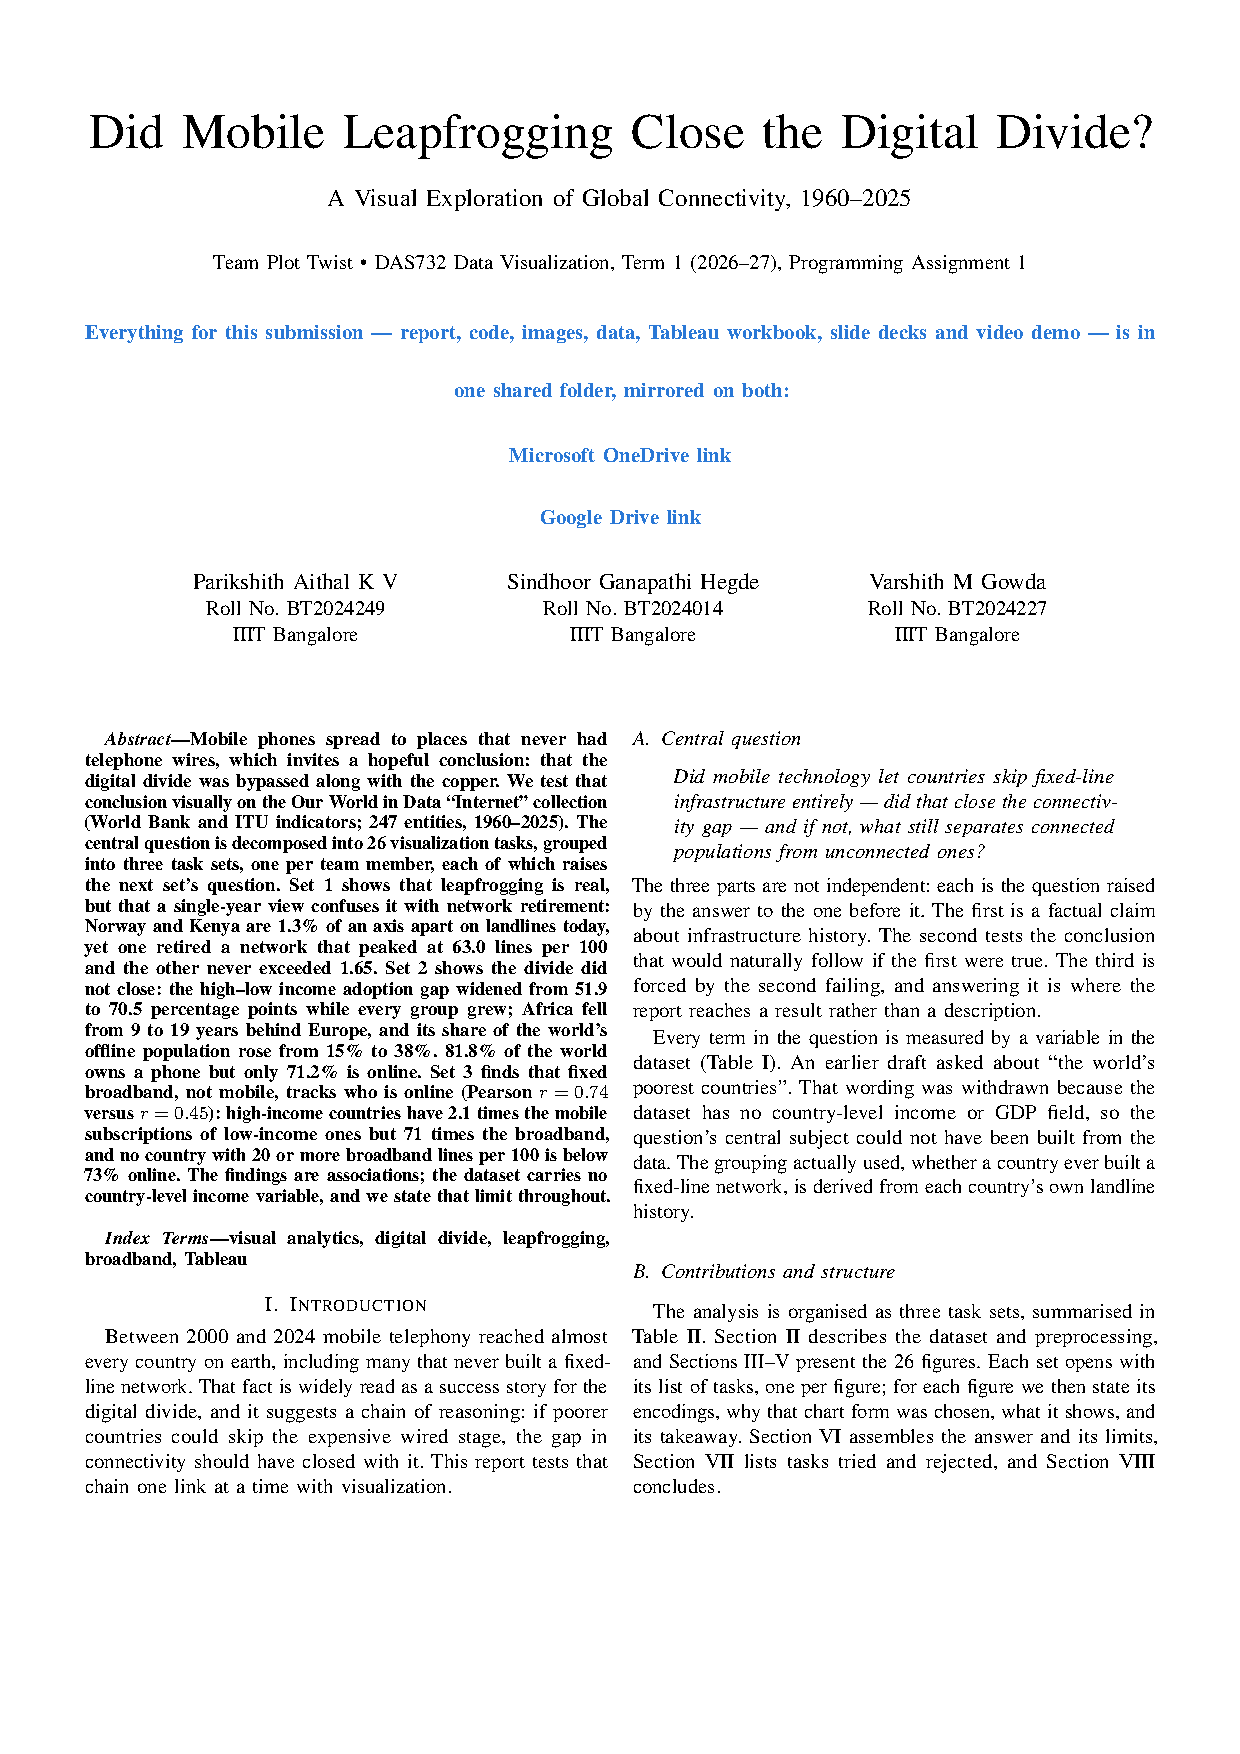
\includepdf[pages=-,scale=0.92,pagecommand={}]{A1_Report_Appendix.pdf}

\end{document}
